%% gWidgets introduction
 
%%\newcommand{\ONLYIN}[1]{[only in #1]}
\newcommand{\Event}[1]{$<$#1$>$}
\newcommand{\VirtualEvent}[1]{$<<$#1$>>$}

\XXX{add in tcl(``source''); external TCL packages}
\XXX{comment about scope -- no user data}


% makeIconTcltk(w, gifFile) {
%   if(as.character(tkwinfo("class", w)) == "Toplevel" &&
%      file.exists(giffile)) {
%     tkimage.create("photo","::icon::name", file=giffile)
%     tcl("wm","iconphoto", w, "::icon::name")
%   }
% }
\chapter{Tcl/Tk: Overview}
\label{sec:tcltk:overview}
\XXX{Where to put loading in external TCL source, packages, ...}
\XXX{tcl("update","idletasks")}
\XXX{use svMisc -- atleast comment on Parse, Complete, CompletePlus}



\TCL\/ (``tool command language'') is a scripting language and
interpreter of that language.  Originally developed in the late 80s by
John Ousterhout as a ``glue'' to combine two or more complicated
applications together, it evolved overtime to find use not just as
middleware, but also as a standalone development tool.

\TK{} is an extension of \TCL\/ that provides GUI components through \TCL.
This was first developed in 1990, again by John Ousterhout. \TK\/
quickly found widespread usage, as, at the time, it made programming GUIs for X11
easier and faster. Over the years, other graphical toolkits have
evolved and surpassed this one, but \TK\/ still has numerous users.

\TK\/ has a large number of bindings available for it,
e.g. \proglang{Perl}, \proglang{Python}, \proglang{Ruby}, and through
the \pkg{tcltk} package, \R. The \pkg{tcltk} package was developed by
Peter Dalgaard and has been included in \R\/ since version 1.1.0. Since then,
the package has been used in a number of GUI projects for \R, most
notably, the \pkg{Rcmdr} GUI. In addition, the \pkg{tcltk2} package
provides additional bindings and bundles in some useful external TCL
code. Our focus here is limited to the base \pkg{tcltk} package.

\TK\/ had a major change between versions 8.4 and 8.5, with the latter
introducing themed widgets. Many widgets were rewritten and their API
dramatically simplified. In \pkg{tcltk} there can be two different
functions to construct a similar widget. For example,
\function{tklabel} or \function{ttklabel}. The latter, with the
\code{ttk} prefix, corresponds to the newer themed variant of the
widget. We assume the \TK\/ version is 8.5 or higher, as this was a
major step forward.\footnote{In fact, we assume version 8.5.8 which
  was the release accompanying \R{} for Windows version 2.13.1.}

Despite its limitations as a graphical toolkit, as compared to \GTK\/
or \Qt, the \TK\/ libraries are widely used for \R\/ GUIs, as for most
users there are no installation issues. \R\/ for Windows has been
bundled with the necessary \TK\/ version for years, so there are no
installation issues for that platform. For Linux users, it is
typically trivial to install the newer libraries and for Mac OS X
users, the provided binary installations include the newer \TK\/
libraries.

%% Documentation sources
\Tk{} has a well documented API\footcite{TclTk:Api}
(\url{www.tcl.tk/man/tcl8.5}).  There are also several books to
supplement. We consulted the one by Welch, Jones and
Hobbs\footcite{beedub} often in the development of this
material. The online sample chapter on geometry management
of Walsh\footcite{Walsh} was perused, as it provides a thorough discussion
of that topic. In addition, the Tk Tutorial of Mark
Roseman\footcite{TclTk:Tutorial} (\url{www.tkdocs.com/tutorial})
provides much detail. \R{} specific documentation include two
excellent R News articles and a proceedings
paper\footcite{Rnews:Dalgaard:2001a}\footcite{Rnews:Dalgaard:2002}\footcite{Dalgaard-DSC}
by Peter Dalgaard, the package author. A
set of examples due to James Wettenhall~\footcite{Wettenhall} are also
quite instructive. A main use of \pkg{tcltk} is within the \pkg{Rcmdr}
framework. Writing extensions for that is well documented in an R News
article~\footcite{Rnews:Fox:2007} by John Fox, the package author.
 

\section{A first example}
\label{sec:first-example}

In this chapter we give an overview of \Tk\/ and \R's interface to it
through the \pkg{tcltk} package using the following small example of a
dialog to collect a name and echo back a message
(Figure~\ref{fig:tcltk-simple-dialog}). In subsequent chapters we give
more detail on the various widgets provided by \Tk.

\begin{figure}
  \centering
  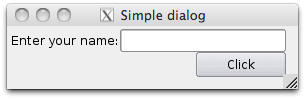
\includegraphics[width=.6\textwidth]{fig-tcltk-themed-dialog.png}
  \caption{A simple dialog to collect a name for later use
    illustrating three basic widgets: a label, entry widget and
    button.}
  \label{fig:tcltk-simple-dialog}
\end{figure}


\begin{Schunk}
\begin{Sinput}
 library(tcltk)
 ##
 w <- tktoplevel()
 tkwm.title(w, "Simple dialog")
 ##
 f <- ttkframe(w, padding=c(3,3,12,12))
 tkpack(f, expand=TRUE, fill="both")
 ##
 g <- ttkframe(f); tkpack(g)
 ##
 l <- ttklabel(g, text="Enter your name:")
 tkpack(l, side="left")
 ##
 txtVar <- tclVar("")
 txt <- ttkentry(g, textvariable=txtVar)
 tkpack(txt)
 ##
 g1 <- ttkframe(f); tkpack(g1, anchor="ne")
 btn <- ttkbutton(g1, text="Click")
 tkpack(btn, side="right")
 ##
 msg <- sprintf("Hello %s", tclvalue(txtVar))
 handler <- function() print(msg)
 tkconfigure(btn, command=handler)
\end{Sinput}
\end{Schunk}
%%
In the above, the first block defines a top-level window and the
second an underlying frame container. We then define and place three
widgets -- a label, entry widget and button -- into a frame. Finally,
we add a callback to respond when the button is clicked.


\section{Interacting with \TCL}
\label{sec:tcltk:interacting-with-tcl}

As the example above makes clear, using \pkg{tcltk} does not
necessarily require knowing anything about the underlying \Tk{} or
\Tcl{} workings, though it can be useful to have a rough sense of these
technologies and how \pkg{tcltk} interfaces with them. As such, we
give a quick overview.


%% Tclk
Although both are scripting languages, the basic syntax of \TCL\/ is
unlike \R. For example a simple string assignment would be made at
tclsh, the \TCL\/ shell with (using \code{\%} as a prompt):
\begin{verbatim}
% set x {hello world}
hello world
\end{verbatim}
Unlike \R\/ where braces are used to form blocks, this example shows
how \TCL\/ uses braces instead of quotes to group the words as a
single string. The use of braces, instead of quotes, in this example
is optional, but in general isn't, as expressions within braces are
not evaluated.  

The example above assigns to the variable \code{x} the
value of \code{hello world}. Once assignment has been made, one can
call commands on the value stored in \code{x} using the \code{\$}
prefix:
\begin{verbatim}
% puts $x
hello world
\end{verbatim}
The \code{puts} command, in this usage, simply writes back its argument to the terminal. Had
we used braces the argument would not have been substituted:
\begin{verbatim}
% puts {$x}
$x
\end{verbatim}

More typical within the \pkg{tcltk} package is the idea of a subcommand. For
example, the \code{string} command provides the subcommand
\code{length} to return the number of characters in the string.
\begin{verbatim}
% string length $x
11
\end{verbatim}

%% .Tcl
The \pkg{tcltk} package provides the low-level function \function{.Tcl} for direct
access to the \TCL\/ interpreter:
\begin{Schunk}
\begin{Sinput}
 library(tcltk)
 .Tcl("set x {some text}")               # assignment
\end{Sinput}
\begin{Soutput}
<Tcl> some text 
\end{Soutput}
\begin{Sinput}
 .Tcl("puts $x")                         # prints to stdout
\end{Sinput}
\end{Schunk}

%% must hard code this, as output isn't printed
\begin{Soutput}
some text
\end{Soutput}

\begin{Schunk}
\begin{Sinput}
 .Tcl("string length $x")                # call a command
\end{Sinput}
\begin{Soutput}
<Tcl> 9 
\end{Soutput}
\end{Schunk}

The \dfn{\function{.Tcl}} function simply sends a command as a text
string to the \TCL\/ interpreter and returns the result as an object
of class \dfn{\class{tclObj}} (cf. \code{?.Tcl}).  The \function{.Tcl}
function can be used to read in \TCL\/ scripts as with
\code{.Tcl("source filename")}. This allows arbitrary \TCL\/ scripts
to run within an \R\/ session. \TCL\/ packages may be read in with
\function{tclRequire}.\footnote{The add-on package \pkg{tcltk2} uses
  both techniques to enhance the base \pkg{tcltk} package with some
  open-source \Tk\/ extensions.}


\paragraph{The \class{tclObj} class}
The \pkg{tcltk} package creates objects with a few different classes,
\iprogram{class structure}\class{tclObj} being the primary one (\class{tclVar} and \class{tkwin}
are two other important ones).  The \class{tclObj} objects print with
the leading \code{<Tcl>}. The string representation of objects of
class \class{tclObj} is returned by \function{tclvalue} or by coercion
through the \function{as.character} function. These two differ in how
they treat spaces and new lines.  Conversion to vectors of mode
\class{character}, \class{double}, \class{integer} and \class{logical}
is possible, though, in general, direct conversion of complicated
\TCL\/ expressions is not supported. One can create objects of this
class through \function{as.tclObj}.



\paragraph{Convenience functions}
The \TK\/ extensions to \TCL\/ have a complicated command structure,
and thankfully, \pkg{tcltk} provides some more conveniently named
functions. To illustrate, the \TCL\/ command to configure the text property for
a label object (\code{.label}) would look like
\begin{verbatim}
% .label configure -text "new text"
\end{verbatim}
The \pkg{tcltk} package provides a corresponding function
\code{tkconfigure}. The above would be done in an \R-like way as (assuming \code{lab} is a
label object):


\begin{Schunk}
\begin{Sinput}
 tkconfigure(lab, text="new text")
\end{Sinput}
\end{Schunk}


% Although the \TCL\/ statement appears to have the object-oriented form
% of ``object method arguments,'' behind the scenes \TCL\/ creates a
% command with the same name as the widget with \code{configure} as a
% subcommand. This is followed by options passed in using the form
% \texttt{-key value}.  


The \TK\/ API for \code{ttklabel}'s \code{configure} subcommand is

\begin{quotation}
  \textit{pathName} \textbf{configure} \textit{?option? ?value option value ...?}
\end{quotation}

The \textit{pathName} is the ID of the label widget. This can be found
from the object \code{l} above, in \code{l\$ID}, or in some cases is a
return value of some other command call.  In the \TK\/ documentation
paired question marks indicate optional values. In this case, one can
specify nothing, returning a list of all options; just an option, to
query the configured value; the option with a value, to modify the
option; and possibly do more than one at at time.  For commands such
as \code{configure}, there will usually correspond a function in
\R\/ of the same name with a \code{tk} prefix, as in this case
\function{tkconfigure}.
% \footnote{The package \pkg{tcltk} was written before
% namespaces were implemented in \R, so the ``tk'' prefix serves that role.}

To make consulting the \TK\/ manual pages easier in the text we would
describe the configure subcommand as
\subcommanda{configure}{ttklabel}{[options]}. (The \R\/ manual pages
simply redirect you to the original \TK\/ documentation, so
understanding this is important for reading the API.) However, if such
a function shortcut is present, we will typically use the shortcut when we
illustrate code. 

Some subcommands have further subcommands. An example
is to set the selection. In the \R\/ function, the second command is
appended with a dot, as in \code{tkselection.set}. (There are a few
necessary exceptions to this.)

\paragraph{The \class{tcl} function} 
Within \pkg{tcltk}, the \function{tkconfigure} function is defined by

\begin{Sinput}
function(widget, ...) tcl(widget, "configure", ...)
\end{Sinput}

The \dfn{\function{tcl}} function is the workhorse used to piece
together \TCL\/ commands, call the interpreter, and then return an
object of class \code{tclObj}.  Behind the scenes it
\begin{itemize}
\item Turns an \R\/
object, \code{widget}, into the \textit{pathName} above (using its ID
component);
\item It passes along strings as subcommands (\code{configure});
\item It converts \R\/ \code{key=value} pairs into \code{-key value}
  options for \TCL. As named arguments are only for the \code{-key
    value} expansion, we follow the \TCL\/ language and call the
  arguments ``options'' in the following. Finally,
\item It adjusts any callback functions allowing \R{} functions and
  expressions to be called.
\end{itemize}
The \function{tcl} function uses position to create its command. The
order of the subcommands needs to match that of the \TK\/ API, so
although it is true that often the \R\/ object is first, this is not
always the case.

\begin{figure}
  \centering
\begin{verbatim}
          tcl(widget, subcommand, key=value, callback)
             /            |           |           \
          widget$ID  subcommand   -key value   makeCallback
\end{verbatim}
  \caption{How the \code{tcl} function maps its arguments}
  \label{fig:tcl-function-map}
\end{figure}






%% constructors

\section{Constructors}
\label{sec:tcltk:constructors}

In this chapter, we will stick to a few basic widgets: labels, entry
widgets, and buttons; to illustrate the  usage of \pkg{tcltk},
leaving for later more detail on containers and widgets.

Unlike \GTK, say, the construction of widgets in \pkg{tcltk} is linked
to the widget hierarchy. \TK\/ widgets are constructed as children of
a parent object with the parent specified to the constructor. When
the \TK\/ shell, wish, is used or the \TK\/ package is loaded through
the \TCL\/ command \code{package require Tk}, a top level window named
``\code{.}'' is created. (This is \code{.TkRoot} in \R.) In the variable name \code{.label}, from
above, the dot refers to the top level window.  In \pkg{tcltk} a
top-level window is created separately through the
\constructor{tktoplevel} constructor, as was done in the example:
\begin{Schunk}
\begin{Sinput}
 w <- tktoplevel()
\end{Sinput}
\end{Schunk}

Top-level windows will be explained in more detail in
Chapter~\ref{sec:tcltk:basic-containers}. 

Other widget constructors require that a parent widget be
specified as the first argument of the constructor.  A typical
invocation was given in the example.
\begin{Schunk}
\begin{Sinput}
 l <- ttklabel(g, text="Enter your name:")
\end{Sinput}
\end{Schunk}
%

\paragraph{Options}
The first argument of a widget constructor is the parent container,
subsequent arguments are used to specify the options for the
constructor given as \code{key=value} pairs. The \TK\/ API lists these
options along with their description.

For a simple label, the following options are possible: \code{anchor},
\code{background}, \code{font}, \code{foreground}, \code{justify},
\code{padding}, \code{relief}, \code{text}, and \code{wraplength}.
This is in addition to the standard options \code{class},
\code{compound}, \code{cursor}, \code{image}, \code{state},
\code{style}, \code{takefocus}, \code{text}, \code{textvariable},
\code{underline}, and \code{width}. (Although clearly lengthy, this
list is significantly reduced from the options for \code{tklabel}
where options for the many style properties are also included.)

Many of the options are clear from their name.  The main option,
\code{text}, takes a character string. The label will be multiline if
this contains new line characters.  The \argument{padding}{ttklabel}
argument allows the specification of space in pixels between the text
of the label and the widget boundary. This may be set as four values
\code{c(left, top, right, bottom)}, or fewer, with \code{bottom}
defaulting to \code{top}, \code{right} to \code{left} and \code{top}
to \code{left}. The \argument{relief}{ttklabel} argument specifies how
a 3-d effect around the label should look, if specified. Possible
values are \qcode{flat}, \qcode{groove}, \qcode{raised},
\qcode{ridge}, \qcode{solid}, or \qcode{sunken}.

\paragraph{The functions \class{tkconfigure}, \class{tkcget}}
Option values may be set through the constructor, or adjusted
afterwards by \function{tkconfigure}. A listing (in \TCL\/ code) of possible options
that can be adjusted may be seen by calling \function{tkconfigure}
with just the widget as an argument.

\begin{Schunk}
\begin{Sinput}
 head(as.character(tkconfigure(l)))      # first 6 only
\end{Sinput}
\begin{Soutput}
[1] "-background frameColor FrameColor {} {}"   
[2] "-foreground textColor TextColor {} {}"     
[3] "-font font Font {} {}"                     
[4] "-borderwidth borderWidth BorderWidth {} {}"
[5] "-relief relief Relief {} {}"               
[6] "-anchor anchor Anchor {} {}"               
\end{Soutput}
\end{Schunk}

The \function{tkcget} function returns the value of an
option (again as a \code{tclObj} object). The option can be specified
two different ways. Either using the \TK\/ style of a leading dash or
using the \R{} convention that \code{NULL} values mean to return the value,
and not set it.


\begin{Schunk}
\begin{Sinput}
 tkcget(l, "-text")                   # retrieve text property
\end{Sinput}
\begin{Soutput}
<Tcl> Enter your name: 
\end{Soutput}
\begin{Sinput}
 tkcget(l, text=NULL)                 # alternate syntax
\end{Sinput}
\begin{Soutput}
<Tcl> Enter your name: 
\end{Soutput}
\end{Schunk}

\paragraph{Coercion to character}
As mentioned, the \code{tclObj} objects can be coerced to characters in two ways.
The conversion through \code{as.character} breaks the return value along whitespace:
\begin{Schunk}
\begin{Sinput}
 as.character(tkcget(l, text=NULL))
\end{Sinput}
\begin{Soutput}
[1] "Enter" "your"  "name:"
\end{Soutput}
\end{Schunk}
%
Whereas, conversion by the \function{tclvalue} function does not:
\begin{Schunk}
\begin{Sinput}
 tclvalue(tkcget(l, text=NULL))
\end{Sinput}
\begin{Soutput}
[1] "Enter your name:"
\end{Soutput}
\end{Schunk}
%

\subsection{The \code{tkwidget} function}
\label{sec:codetkw-funct}


Constructors call the \function{tkwidget} function which returns an
object of class \code{tkwin}. (In \TK\/ the term ``window'' is used to
refer to the drawn widget and not just a top-level window). E.g.,

\begin{Schunk}
\begin{Sinput}
 str(btn)
\end{Sinput}
\begin{Soutput}
List of 2
 $ ID : chr ".1.1.2.1"
 $ env:<environment: 0x1032bacd8> 
 - attr(*, "class")= chr "tkwin"
\end{Soutput}
\end{Schunk}

The returned widget objects are lists with two components: an ID and an
environment. The \code{ID} component keeps a unique ID of the
constructed widget. This is a character string, such as ``.1.2.1''
coming from the the widget hierarchy of the object. This value is
generated behind the scenes by the \pkg{tcltk} package using numeric
values to keep track of the hierarchy. The \code{env} component
contains an environment that keeps a count of the subwindows, the parent
window and any callback functions. This helps ensure that any copies
of the widget refer to the same object~\footcite{Dalgaard-DSC}. As the
construction of a new widget requires the \code{ID} and environment of
its parent, the first argument to \function{tkwidget} (and hence any constructor), \code{parent},
must be a \class{tkwin} object, not simply its character ID, as is
possible for the \function{tcl} function.

%%The latter is useful in
%%a callback, as only the ID may be known to the callback function.

\subsection{Geometry managers}
\label{sec:tcltk:overview:geometry-managers}

In the example we saw several calls to \code{tkpack}. For example,

\begin{Schunk}
\begin{Sinput}
 tkpack(f, expand=TRUE, fill="both")
 tkpack(l, side="left")
 tkpack(txt)
 g1 <- ttkframe(f); tkpack(g1, anchor="ne")
\end{Sinput}
\end{Schunk}


As with \Qt, when a new widget is constructed it is not automatically
mapped. \TK\/ uses geometry managers to specify how the widget will be
drawn within the parent container. We will discuss two such geometry
managers, \code{tkpack} and \code{tkgrid}, in Chapter~\ref{sec:tcltk:basic-containers}.

The \code{tkpack} command packs the widgets into the parent container
in a box-like manner. The example shows various arguments that adjust
the position of the child component and how space is to be allocated
when an excess of space is present.



\subsection{\TCL\/ variables}
\label{sec:tcltk:overview:textvariables}


%% textvariables
For the button and label widgets in our example, their \code{text}
property is configured through calls to their constructors. Many
widgets allow an alternative way to specify one or two important
properties using an independent \Tcl\/ variable.

In the call to \code{ttkentry} in the example we had:

\begin{Schunk}
\begin{Sinput}
 txtVar <- tclVar("")
 txt <- ttkentry(g, textvariable=txtVar)
\end{Sinput}
\end{Schunk}
%
The first line defines a new object of class \class{tclVar} which is
used for the \code{textvariable} option when defining the entry
widget. This variable is dynamically bound to the widget, so that
changes to the variable are propagated to the GUI. (The \TCL\/
variable is a model and the widget a view of the model.)  The \Tcl{}
variable may be used with more than one widget, allowing a simple form
of synchronization.

The basic functions involved are \function{tclVar} to create a \TCL\/
variable, \function{tclvalue} to get the assigned value and
\function{tclvalue\ASSIGN} to modify the value.

\begin{Schunk}
\begin{Sinput}
 tclvalue(txtVar) <- "Somebody's name"
 tclvalue(txtVar)
\end{Sinput}
\begin{Soutput}
[1] "Somebody's name"
\end{Soutput}
\end{Schunk}

\TCL\/ variables have a unique identifier, returned by \function{as.character}:
\begin{Schunk}
\begin{Sinput}
 as.character(txtVar)
\end{Sinput}
\begin{Soutput}
[1] "::RTcl1"
\end{Soutput}
\end{Schunk}

The advantages of \TCL\/ variables are like those of the MVC paradigm
-- a single data source can have its changes propagated to several
widgets automatically. If the same text is to appear in different
places, their usage is recommended.  One disadvantage, is that in a
callback, the variable is not passed to the callback and can't be
recovered from the object itself. Hence, it must be found
through \R's scoping rules. (In Section~\ref{sec:tcltk:checkboxes} we
show a workaround.)

The package also provides the function \dfn{\function{tclArray}} to
store an array of \TCL\/ variables. The usual list methods \code{[[}
and \code{\$} and their forms for assignment are available for arrays,
but values are only referred to by name, not index:



\begin{Schunk}
\begin{Sinput}
 x <- tclArray()                    # no init
 x$one <- 1; x[[2]] <- 2            # $<- and [[<-
 x[[1]]                             # no match by index
\end{Sinput}
\begin{Soutput}
NULL
\end{Soutput}
\begin{Sinput}
 names(x)                           # the stored names
\end{Sinput}
\begin{Soutput}
[1] "2"   "one"
\end{Soutput}
\begin{Sinput}
 x[['2']]                           # match by name, not index
\end{Sinput}
\begin{Soutput}
<Tcl> 2 
\end{Soutput}
\end{Schunk}



\subsection{Commands}
\label{sec:tcltk-intro-commands}


In the definition of the button we saw:

\begin{Schunk}
\begin{Sinput}
 btn <- ttkbutton(g1, text="Click")
 #
 msg <- sprintf("Hello %s", tclvalue(txtVar))
 handler <- function() print(msg)
 tkconfigure(btn, command=handler)
\end{Sinput}
\end{Schunk}

Button widgets are used to initiate  some action, or
command, and the \code{command} option is used to specify this. This
may be given as a function or expression, though we only illustrate
the former. The command is invoked by clicking and releasing the mouse
on the button, by pressing the space bar when the button has the focus
or by calling the widget's \subcommand{invoke}{ttkbutton}
subcommand. 

The \code{command} option is available for many widgets, but is not
the only means to invoke a function call, as \Tk{} also allows one to
bind to various types of events, e.g., button clicks.  More on
callbacks in \pkg{tcltk} will be explained in
Section~\ref{sec:tcltk:callbacks}.




\subsection{Themes}
\label{sec:tcltk:overview:themes}


%% themes -- ttkframe
As mentioned, the newer themed widgets have a style that determines
how they are drawn based on the state of the widget. The separation of
style properties from the widget, as opposed to having these set for
each construction of a widget, makes it much easier to change the look
of a GUI and easier to maintain the code. A collection of styles makes
up a theme. The available themes depend on the system. The default
theme allows the GUI to have the native look and feel of the operating
system. (This was definitely not the case for the older \TK\/
widgets.)

In our example, the toplevel window has a frame immediately packed
inside of it through the commands:
\begin{Schunk}
\begin{Sinput}
 w <- tktoplevel()
 f <- ttkframe(w, padding=c(3,3,12,12))
 tkpack(f, expand=TRUE, fill="both")
\end{Sinput}
\end{Schunk}

\begin{figure}
  \centering
  \begin{minipage}[c]{.45\linewidth}
    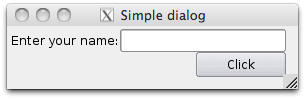
\includegraphics[width=\textwidth]{fig-tcltk-themed-dialog.png}    
  \end{minipage}\quad
  \begin{minipage}[c]{.45\linewidth}
   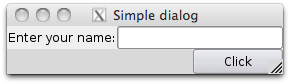
\includegraphics[width=\textwidth]{fig-tcltk-non-themed-dialog.png}
 \end{minipage}
 \caption{Comparison of themed versus non-themed dialog. The right
    one does not use an inner \code{ttkframe} and in addition to not
    having padding, has a mismatched color.}
  \label{fig:tcltk-compare-themed-non-themed}
\end{figure}


The arguments to \code{tkpack} are given so that the frame, \code{f},
will expand and fill all the space allocated by the toplevel
window. As the toplevel window is not a themed widget, not doing this
can leave odd-looking effects~\ref{fig:tcltk-compare-themed-non-themed}.

%% Workign with thems
There is no built in command to return the theme, so we use
\code{.Tcl} to call the appropriate \code{names}
sub command:

\begin{Schunk}
\begin{Sinput}
 .Tcl("ttk::style theme names")
\end{Sinput}
\begin{Soutput}
<Tcl> clam alt default classic 
\end{Soutput}
\end{Schunk}
%
The \code{use} sub command is used to set the theme:
\begin{Schunk}
\begin{Sinput}
 .Tcl("ttk::style theme use clam")
\end{Sinput}
\end{Schunk}

\paragraph{State of themed widgets}

The themed widgets (those with a \code{ttk} constructor) have a state
to determine which style is to be applied when painting the
widget. These states can be adjusted through the \code{state} command
and queried with the \code{instate} command. For example, to see if
button widget \code{b} has the focus we have:
\begin{Schunk}
\begin{Sinput}
 as.logical(tcl(btn, "instate", "focus"))
\end{Sinput}
\begin{Soutput}
[1] FALSE
\end{Soutput}
\end{Schunk}
To set a widget to be not sensitive to user input we have:
\begin{Schunk}
\begin{Sinput}
 tcl(btn, "state", "disabled")             # not sensitive
\end{Sinput}
\begin{Soutput}
<Tcl> !disabled 
\end{Soutput}
\end{Schunk}
The states are bits and can be negated by prefacing the value with \code{!}:
\begin{Schunk}
\begin{Sinput}
 tcl(btn, "state", "!disabled")            # sensitive again
\end{Sinput}
\begin{Soutput}
<Tcl> disabled 
\end{Soutput}
\end{Schunk}

The full list of states is in the manual page for \code{ttk::widget}.


The writing of themes will not be covered, but in
Example~\ref{ex-tcltk-toolbar} we show how to create a new style for a
button. This topic is covered in some detail in the \Tk\/ tutorial by Roseman.
\\

% The example we have shown so far, would not look quite right for some
% operating systems, as the toplevel window is not a themed widget
% (Figure~\ref{fig:tcltk-frame-noframe-example}). To work around that, a
% \function{ttkframe} widget is usually used to hold the child
% components of the top-level window. The following shows how to place a
% frame inside the window, with some arguments to be explained later
% that allow it to act reasonably if the window is resized.

% \begin{figure}
%   \centering
%   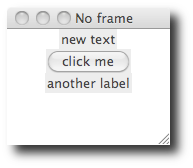
\includegraphics[width=.4\textwidth]{fig-tcltk-no-frame}
%   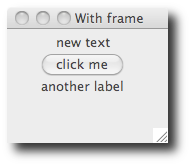
\includegraphics[width=.4\textwidth]{fig-tcltk-with-frame}
%   \caption{Similar GUIs, one using a frame within the toplevel window
%     (right one) and one without. The one without has widgets whose background does not match the toplevel window.}
%   \label{fig:tcltk-frame-noframe-example}
% \end{figure}


% <<no-frame, echo=FALSE>>=
% w <- tktoplevel()
% tkwm.title(w, "No frame")
% l <- ttklabel(w, text="new text")
% tkpack(l)

% b <- ttkbutton(w, text="click me", 
%                command=function() print("thanks"))
% tkpack(b)

% textvar <- tclVar("another label")
% l2 <- ttklabel(w, textvariable=textvar)
% tkpack(l2)
% @ 

% <<with-frame, echo=FALSE>>=
% w <- tktoplevel()
% tkwm.title(w, "With frame")
% w <- ttkframe(w, padding=c(3,3,12,12))  # Some breathing room
% tkpack(w, expand=TRUE, fill="both")     # For window expansion
% l <- ttklabel(w, text="new text")
% tkpack(l)

% b <- ttkbutton(w, text="click me", 
%                command=function() print("thanks"))
% tkpack(b)

% textvar <- tclVar("another label")
% l2 <- ttklabel(w, textvariable=textvar)
% tkpack(l2)
% @ 

% <<UseFrameToTheme>>=
% w <- tktoplevel()
% f <- ttkframe(w, padding=c(3,3,12,12))  # Some breathing room
% tkpack(f, expand=TRUE, fill="both")     # For window expansion
% l <- ttklabel(f,  text="label")         # some widget
% tkpack(l)
% @ 


\subsection{Window properties and state: \code{tkwinfo}}
\label{sec:tcltk:overview:widget-properties}

For a widget, the function \function{tkcget} is used to get the values
of its options. If it is a themed widget, the \code{instate} command
returns its state values. 

To query the values of the containing window of the widget the
\function{tkwinfo} function is used.  When widgets are mapped, the
``window'' they are rendered to has properties, such as a class or
size. There are a few subcommands provided by \pkg{tcltk}, but by no
means is this exclusive. Rather, one can pass in the subcommand as an
argument to \function{tkwinfo}. If the subcommand's API is of the form

\begin{quotation}
\texttt{winfo} \textbf{subcommand\_name} \textit{window}  
\end{quotation}
the specification to \function{tkwinfo} is in the same order (the
widget is not the first argument). For instance, the
class\footnote{The class of a widget is more like a attribute and should
  not be confused with class in the object oriented sense. The class
  is used internally for bindings and styles.} of a label
is returned by the \texttt{class} subcommand:

\begin{Schunk}
\begin{Sinput}
 tkwinfo("class", l)
\end{Sinput}
\begin{Soutput}
<Tcl> TLabel 
\end{Soutput}
\end{Schunk}
%

The window, in this example \texttt{l}, can be specified as an \R\/
object, or by its character ID. This is useful, as the return value of
some functions is the ID. For instance, the \texttt{children}
subcommand returns IDs. Below the \code{as.character} function will
coerce these into a vector of IDs.


\begin{Schunk}
\begin{Sinput}
 (children <- tkwinfo("children", w))
\end{Sinput}
\begin{Soutput}
<Tcl> .4.1 .4.2 
\end{Soutput}
\begin{Sinput}
 sapply(as.character(children), function(i) tkwinfo("class", i))
\end{Sinput}
\begin{Soutput}
$`.4.1`
<Tcl> TButton 

$`.4.2`
<Tcl> TButton 
\end{Soutput}
\end{Schunk}

There are several possible subcommands, here we list a few. The
\subcommand{geometry}{tkwinfo} sub command returns the location and
size of the widgets' window in the form \code{width x height + x + y};
the sub commands \subcommand{height}{tkwinfo},
\subcommand{width}{tkwinfo}, \subcommand{x}{tkwinfo}, or
\subcommand{y}{tkwinfo} can be used to return just those parts. The
\subcommand{exists}{tkwinfo} command returns 1 (\code{TRUE}) if the
window exists and 0 otherwise; the \subcommand{ismapped}{tkwinfo} sub
command returns 1 or 0 if the window is currently mapped (drawn); the
\subcommand{viewable}{tkwinfo} sub command is similar, only it checks
that all parent windows are also mapped.  

\iprogram{widget hierarchy}
For traversing the widget hierarchy, one has available the
\subcommand{parent}{tkwinfo} sub command which returns the immediate
parent of the component, \subcommand{toplevel}{tkwinfo} which returns
the ID of the top-level window, and \subcommand{children}{tkwinfo}
which returns the IDs of all the immediate child components, if the
object is a container, such as a top-level window.


\subsection{Colors and fonts}
\label{sec:tcltk:overview:colors-fonts}
Colors and fonts are typically specified through a theme, but at times
it is desirable to customize the preset ones.

The label color can be set through its \code{foreground}
property. Colors can be specified by name -- for common colors -- or
by hex RGB values which are common in web programming.
\begin{Schunk}
\begin{Sinput}
 tkconfigure(l, foreground="red")
 tkconfigure(l, foreground="#00aa00")
\end{Sinput}
\end{Schunk}

To find the hex RGB value, one can use the \code{rgb} function to
create RGB values from intensities in $[0,1]$.  The \R\/ function
\function{col2rgb} can translate a named color into RGB values. The
\code{as.hexmode} function will display an integer in hexadecimal
notation.

In Example~\ref{ex:tcltk-entry-initial-message} we show how to modify
a style, as opposed to the \code{foreground} option, to change the
text color in an entry widget.

%% fonts
\paragraph{Fonts}
Fonts are a bit more involved than colors. \TK\/ version 8.5 made it
more difficult to change font properties of individual widgets, this
following the practice of centralizing style options for consistency,
ease of maintaining code and ease of theming.  To set a font for a
label, rather than specifying the font properties, one configures the
\code{font} options using a pre-defined font name, such as
\begin{Schunk}
\begin{Sinput}
 tkconfigure(l, font="TkFixedFont")
\end{Sinput}
\end{Schunk}

The \qcode{TkFixedFont} value is one of the standard font names, in
this case to use a fixed-width font. A complete list of the standard
names is provided in Table~\ref{tab:tcltk-std-fonts}. Each theme sets
these defaults accordingly.
\begin{table}
\centering
\label{tab:tcltk-std-fonts}
\caption{Standard font names defined by a theme.}
\begin{tabular}{@{}ll@{}}
\toprule

Standard font name&Description\\
\midrule
\code{TkDefaultFont}&Default font for all GUI items not otherwise specified\\\code{TkTextFont}&Font for text widgets\\\code{TkFixedFont}&Fixed-width font\\\code{TkMenuFont}&Menubar fonts\\\code{TkHeadingFont}&Font for column headings\\\code{TkCaptionFont}&Caption font (dialogs)\\\code{TkSmallCaptionFont}&Smaller caption font\\\code{TkIconFont}&Icon and text font
\\ \bottomrule
\end{tabular}
\end{table}%
\paragraph{Using \code{tkfont.create}}
The \index{tkfont!\code{create}} \function{tkfont.create} function can be used to create a new font, as with the following commands:
\begin{Schunk}
\begin{Sinput}
 tkfont.create("ourFont", family="Helvetica", size=12, 
               weight="bold")
\end{Sinput}
\begin{Soutput}
<Tcl> ourFont 
\end{Soutput}
\begin{Sinput}
 tkconfigure(l, font="ourFont")
\end{Sinput}
\end{Schunk}

As font families are system dependent, only \qcode{Courier},
\qcode{Times} and \qcode{Helvetica} are guaranteed to be there. A list
of an installation's available font families is returned by the
function \function{tkfont.families}.
Figure~\ref{fig:fig-tcltk-all-fonts} shows a display of some available
font families on a Mac OS X machine.  See
Example~\ref{ex:tcltk-scrollable-frame} for details.

The arguments for \function{tkfont.create} are optional. The
\argument{size}{tkfont.create} argument specifies the pixel size. The
\argument{weight}{tkfont.create} argument can be used to specify
\qcode{bold} or \qcode{normal}.  Additionally, a
\argument{slant}{tkfont.create} argument can be used to specify either
\qcode{roman} (normal) or \qcode{italic}. Finally,
\argument{underline}{tkfont.create} and
\argument{overstrike}{tkfont.create} can be set with a \code{TRUE} or
\code{FALSE} value.


\begin{figure}
  \centering
  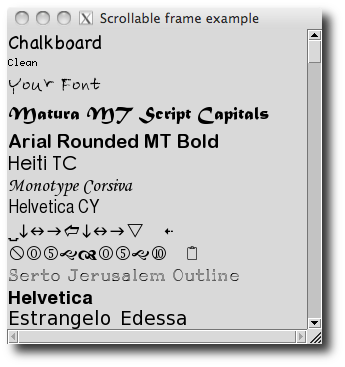
\includegraphics[width=.6\textwidth]{fig-tcltk-all-fonts.png}
  \caption{A scrollable frame widget (cf. Example~\ref{ex:tcltk-scrollable-frame}) showing the available fonts on a system.}
  \label{fig:fig-tcltk-all-fonts}
\end{figure}


\paragraph{Font metrics}
The average character size is important in setting the width and
height of some components. (For example the text widget specifies its
height in lines, not pixels.) These sizes can be found using the
\function{tkfont.measure} and \function{tkfont.metrics}. Although the
average text size varies for proportional fonts, the size of the
\code{M} character is often used.
\begin{Schunk}
\begin{Sinput}
 font_measure <- tcl("font","measure","TkTextFont","M")
 fontWidth <- as.integer(tclvalue(font_measure))
 tmp <- tkfont.metrics("TkTextFont","linespace"=NULL)
 fontHeight <- as.numeric(tclvalue(tmp))
 #
 c(width=fontWidth, height=fontHeight)
\end{Sinput}
\begin{Soutput}
 width height 
    10     15 
\end{Soutput}
\end{Schunk}


\subsection{Images}
\label{sec:tcltk:overview:images}


Many \pkg{tcltk} widgets, including both labels and buttons, can show
images. In these cases, either with or without an accompanying text
label. Constructing images to display is similar to constructing new
fonts, in that a new image object is created and can be reused by
various widgets. This shared use of resources reduces memory
consumption, and is an example of the flyweight design pattern.
\\

Images are created by the \function{tkimage.create} function.
The following command shows how an image object can be made from the
file \code{tclp.gif} in the current directory:

\begin{Schunk}
\begin{Sinput}
 tkimage.create("photo", "::img::tclLogo", file = "tclp.gif")
\end{Sinput}
\begin{Soutput}
<Tcl> ::img::tclLogo 
\end{Soutput}
\end{Schunk}


The first argument, \qcode{photo} specifies that a full color image is
being used. (This option could also be \qcode{bitmap} but that is more
a legacy option.)\footnote{The \pkg{tkrplot} package allows a third
  option \code{Rplot}. This package has the high-level command
  \function{tkrplot}, but the low-level use of a) calling
  \code{.my.tkdev(hscale=1,vscale=1)} b) creating a graphic and c) creating an image
  object through \code{tkimage.create("Rplot", img\_name)} will
  produce a new image object one can use.} The second argument
specifies the name of the object. We follow the advice of the \TK\/
manual and preface the name with \code{::img::} so that we don't
inadvertently overwrite any existing \TCL\/ commands. (The command
\code{tcl("image", "names")} will return all defined image names.) The
third argument \argument{file}{tkimage.create} specifies the graphic
file. The basic \TK\/ \code{image} command can only show GIF and
PPM/PNM images. Unfortunately, not many \R\/ devices output in these
formats. (The \code{GDD} device driver can.) One may need system
utilities to convert to the allowable formats or install add-on \TCL\/
packages that can display other formats.~

To use the image, one specifies the image name to the
\option{image}{ttklabel} option:
\begin{Schunk}
\begin{Sinput}
 l <- ttklabel(w, image="::img::tclLogo", text="logo text", 
               compound = "top")
\end{Sinput}
\end{Schunk}

By default the text will not show. The \argument{compound}{ttklabel}
argument takes a value of either \qcode{text}, \qcode{image}
(default), \qcode{center}, \qcode{top}, \qcode{left}, \qcode{bottom},
or \qcode{right} specifying where the label is in relation to the
text.

\paragraph{Image manipulation}
Once an image is created, there are several options to manipulate the
image. These are found in the \TK\/ man page for \code{photo}, not
\code{image}. For instance, to change the palette so that instead of
\code{fullcolor} only 16 shades of gray are used to display the icon,
one could issue the command
\begin{Schunk}
\begin{Sinput}
 tkconfigure("::img::tclLogo", palette=16)
\end{Sinput}
\end{Schunk}

%% changed to active, !active
% Another useful manipulation to draw attention to an image is to change
% the \code{gamma} value when something happens, such as a mouse-over
% event (cf. Example~\ref{ex-tcltk-toolbar}).



\section{Events and callbacks}
\label{sec:tcltk:overview:events-callbacks}

The button widget has the \code{command} option for assigning a
callback which is invoked (among other ways) when the user clicks the
mouse on the button. In addition to such commands, one may use
\function{tkbind} to invoke callbacks in response to many other events
that the user may initiate. The basic call is \code{tkbind(tag, event, script)}. 

%% (Unlike \pkg{RGtk2}, that the event triggers a widget to emit a signal that a callback listens for is not needed)

\subsection{The tag}

The \code{tag} object is more general than just a widget, or its
id. It can be:

\begin{description}
\item[the name of a widget,] in which case the command will be bound to that widget;
\item[a top-level window,] in which case the command will be be bound
  to the event for the window and all its internal widgets;
\item[a class of widget,] such as \qcode{TButton}, in which case all
  such widgets will get the binding; or
\item[the value \qcode{all},] in which case all widgets in the
  application will get the binding.
\end{description}

This flexibility makes it easy to create keyboard accelerators. For
example, the following mimics the linux shortcut \code{Control-q} to
close a window.
\begin{Schunk}
\begin{Sinput}
 w <- tktoplevel()
 b <- ttkbutton(w, text="Some widget with the focus")
 tkpack(b)
 tkbind(w, "<Control-q>", function() tkdestroy(w))
\end{Sinput}
\end{Schunk}
%
By binding to the top-level window, we ensure that no matter which
widget has the focus the command will be invoked by the keyboard shortcut.


\subsection{Events}
\label{sec:tcltk:events}
\iprogram{signals}

%% possible events
%% keys
Of course, the possible events (or sequences of events) vary from widget to
widget. In addition, these events can be specified in a few ways. 

The example below uses two types of events. A single key press event, such as
``C'' or ``O'' can invoke a command and is specified by just its
character. Whereas, the event of pressing the return key is specified
using \code{\event{Return}}. In the following we bind the key presses to the
top-level window and the return event to any button with the default
class \code{TButton}.

\begin{Schunk}
\begin{Sinput}
 w <- tktoplevel()
 l <- ttklabel(w, text="Click Ok for a message")
 b1 <- ttkbutton(w, text="Cancel", 
                 command=function() tkdestroy(w))
 b2 <- ttkbutton(w, text="Ok", command=function() {
   print("initiate an action")
 })
 sapply(list(l,b1,b2), tkpack)
 ##
 tkbind(w, "C", function() tcl(b1, "invoke"))
 tkconfigure(b1, underline=0)
 ##
 tkbind(w, "O", function() tcl(b1, "invoke"))
 tkconfigure(b2, underline=0)
 tkfocus(b2)
 ##
 tkbind("TButton", "<Return>", function(W) {
   tcl(W, "invoke")
 })
\end{Sinput}
\end{Schunk}
%
We modified our buttons using the \code{underline} option to give the
user an indication that the ``C'' and ``O'' keys will initiate some
action (Figure~\ref{fig:tcltk-underline-buttons}). Our callbacks
simply cause the appropriate button to \code{invoke} their
command. The latter one uses a percent substitution (below), which is
how \TK\/ passes along information about the event to the callback.

\begin{figure}
  \centering
  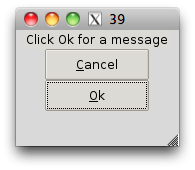
\includegraphics[width=.35\textwidth]{fig-tcltk-underline-buttons.png}
  \caption{Simple GUI showing buttons with \code{underline}
    property. The underlined letters match bindings to the top level
    window to invoke the button.}
  \label{fig:tcltk-underline-buttons}
\end{figure}

%% tkbind(widget,''<modifier-modifier-type-detail'>'', command)
\paragraph{Events with modifiers}
More complicated events can be described with the pattern

\begin{quotation}
\code{\Event{modifier-modifier-type-detail}}.   
\end{quotation}

Examples of a ``type'' are \code{\Event{KeyPress}} or
\code{\Event{ButtonPress}}. The event \code{\Event{Control-q}}, used
above, has the type \code{q} and modifier \code{Control}. Whereas
\code{\Event{Double-Button-1}} uses the detail \code{1} to indicate
which mouse button. The full list of modifiers and types are described
in the man page for \code{bind}. Some familiar modifiers are
\code{Control}, \code{Alt}, \code{Double} and \code{Triple}. The event
types are the standard X event types along with some
abbreviations. These are also listed in the \code{bind} man page. Some
commonly used ones are \code{Return} (as above), \code{ButtonPress},
\code{ButtonRelease}, \code{KeyPress}, \code{KeyRelease},
\code{FocusIn}, and \code{FocusOut}.

\paragraph{Window manager events}\iprogram{window manager events}
Some events are based on window manager events. The \code{\Event{Configure}}
event happens when a component is resized. The \code{\Event{Map}} and
\code{\Event{Unmap}} events happen when a component is drawn or undrawn.

\paragraph{Virtual events}
Finally, the event may be a ``virtual event.'' These are represented
as \code{\VirtualEvent{EventName}}. There are predefined virtual
events listed in the \code{event} man page. These include
\code{\VirtualEvent{MenuSelect}} when working with menus,
\code{\VirtualEvent{Modified}} for text widgets,
\code{\VirtualEvent{Selection}} for text widgets, and
\code{\VirtualEvent{Cut}}, \code{\VirtualEvent{Copy}} and
\code{\VirtualEvent{Paste}} for working with the clipboard. New
virtual events can be produced with the \code{tkevent.add}
function. This function takes at least two arguments, an event name and a
sequence that will initiate that event. The \code{event} man page has
these examples coming from the Emacs world:
\begin{Schunk}
\begin{Sinput}
  tkevent.add("<<Paste>>", "<Control-y>")
  tkevent.add("<<Save>>", "<Control-x><Control-s>")
\end{Sinput}
\end{Schunk}
%
In addition to virtual events occurring when the sequence is performed,
the \function{tkevent.generate} can be used to force an event for a
widget. This function requires a widget (or its ID) and the event
name. Other options can be used to specify substitution values,
described below. To illustrate, this command will generate the
\code{\VirtualEvent{Save}} event for the button \code{btn}:
\begin{Schunk}
\begin{Sinput}
 tkevent.generate(btn, "<<Save>>")
\end{Sinput}
\end{Schunk}
%
Example~\ref{ex-tcltk-dnd} uses virtual events to implement drag and
drop features.


\subsection{Callbacks}
\label{sec:tcltk:callbacks}
%% \XXX{ use of tcl(``eval'',''break'') to avoid calling subsequent callbacks} -- doesn't work
%% See PD's comments here on callbacks http://article.gmane.org/gmane.comp.lang.r.general/136705

\iprogram{event handlers}
The \pkg{tcltk} package implements callbacks in a manner different
from \TK, as the callback functions are \R\/ functions, not \TK\/
procedures. This is much more convenient, but introduces some slight
differences.  In \pkg{tcltk} these callbacks can be expressions
(unevaluated calls) or functions. We use only the latter. The basic
callback function need not have any arguments and those that do only
have percent substitutions passed in.


%% scope of callback?
The callback's return value is generally not important, although we
shall see that within the validation framework of entry widgets
(Section~\ref{sec:tcltk:entry-widgets}) it can matter.\footnote{The
  difference in processing of return values can make porting some
  \Tk\/ code to \pkg{tcltk} difficult. For example, the \code{break}
  command to stop a chain of call backs does not work.}



In \pkg{tcltk} only one callback can be associated with a widget and
event through the call
\code{tkbind(widget,event,callback)}. (Although, callbacks for the
widget associated with classes or toplevel windows can differ.)
Calling \code{tkbind} another time will replace the callback. To
remove a callback, simply assign a new callback which does
nothing.\footnote{This event handling can prevent one being able to port
  some \Tk\/ code into \pkg{tcltk}. In those cases, one may consider
  sourcing in \Tcl\/ code directly.}



\subsection{\% Substitutions}
\label{sec:tcltk-percent-substitutions}

One can not pass arbitrary user data to a callback, rather such values
must be found through \R's usual scoping rules. However, \TK\/
provides a mechanism called \defn{percent substitution} to pass
information about the event to callbacks bound to the event. The basic
idea is that in the \TCL\/ callback expressions of the type
\code{\%X}, for different characters \code{X}, will be replaced by values
coming from the event. In \pkg{tcltk}, if the callback function has an
argument \code{X}, then that variable will correspond to the value
specified by \code{\%X}. The complete list of substitutions is in the
\code{bind} man page. Some useful ones are \code{x} and \code{X} to
specify the relative or absolute $x$-postion of a mouse click (the
difference can be found through the \code{rootx} property of a
widget), \code{y} and \code{Y} for the $y$-position, \code{k} and
\code{K} for the keycode (ASCII) and key symbol of a
\code{\Event{KeyPress}} event, and \code{W} to refer to the ID of the
widget that signaled the event the callback is bound
to. 

The following trivial example illustrates, whereas
Example~\ref{ex-tcltk-dnd} will put these to use.

\begin{Schunk}
\begin{Sinput}
 w <- tktoplevel()
 b <- ttkbutton(w, text="Click me to record the x,y position")
 tkpack(b)
 tkbind(b, "<ButtonPress-1>", function(W, x, y, X, Y) {
   print(W)                              # an ID
   print(c(x, X))                        # character class
   print(c(y, Y))
   })
\end{Sinput}
\end{Schunk}




%% After
\paragraph{The after command}
The \TCL\/ command \iprogram{timers}\code{after} will execute a command after a certain
delay (specified in milliseconds as an integer) while not interrupting
the control flow while it waits for its delay. The function is called
in a manner like:
\begin{Schunk}
  \begin{Sinput}
ID <- tcl("after", 1000, function() print("1 second passed"))    
  \end{Sinput}
\end{Schunk}
The ID returned by \code{after} may be used to \code{cancel} the
command before it executes. To execute a command repeatedly, can be
done along the lines of:
\begin{Schunk}
\begin{Sinput}
 afterID <- ""
 someFlag <- TRUE
 repeatCall <- function(ms=100, f) {
   afterID <<- tcl("after", ms, function() {
     if(someFlag) {                      
       f()
       afterID <<- repeatCall(ms, f)
     }  else {
       tcl("after", "cancel", afterID)
     }
   })
 }
 repeatCall(2000, function() {
   print("Running. Set someFlag <- FALSE to stop.")
 })
\end{Sinput}
\end{Schunk}
%


\begin{example}{Drag and drop}{ex-tcltk-dnd}
This relatively involved example\footnote{The idea for the example
  code originated with \url{http://wiki.tcl.tk/416}} shows several
different uses of the event framework to implement drag and drop
behavior between two widgets. It certainly may be skipped on first reading.


In \pkg{tcltk} much more work is involved with drag and drop, than
with \pkg{RGtk2} and \pkg{qtbase}, as there are no predefined methods
to facilitate the process. 

Here we go through the steps needed to make one widget a drop source,
and the other a drop target The basic idea is that when a value is
being dragged, virtual events are generated for the widget the cursor
is over. If that widget has callbacks listening to these events, then the
drag and drop can be processed.


To begin, we create a simple GUI to hold three widgets. We use buttons
for drag and drop, but only for convenience. Other widgets would be
used in a real application.
\begin{Schunk}
\begin{Sinput}
 w <- tktoplevel()
 bDrag <- ttkbutton(w, text="Drag me")
 bDrop <- ttkbutton(w, text="Drop here")
 tkpack(bDrag)
 tkpack(ttklabel(w, text="Drag over me"))
 tkpack(bDrop)
\end{Sinput}
\end{Schunk}
%

Before beginning, we define three global variables that can be shared
among drop sources to keep track of the drag and drop state. 
\begin{Schunk}
\begin{Sinput}
 .dragging <- FALSE                 # currently dragging?
 .dragValue <- ""                   # value to transfer
 .lastWidgetID <- ""                # last widget dragged over
\end{Sinput}
\end{Schunk}
%
%
To set up a drag source, we bind to three events: a mouse button
press, mouse motion, and a button release. For the button press, we
set the values of the three global variables.
\begin{Schunk}
\begin{Sinput}
 tkbind(bDrag,"<ButtonPress-1>",function(W) {
   .dragging <<-  TRUE
   .dragValue <<- as.character(tkcget(W,text=NULL))
   .lastWidgetID <<- as.character(W)
 })
\end{Sinput}
\end{Schunk}
%
This initiates the dragging immediately. A more common strategy is to
record the position of the mouse click and then initiate the dragging
after a certain minimal movement is detected.

%
For mouse motion, we do several things. First we set the cursor to
indicate a drag operation. The choice of cursor is a bit outdated. The
comment refers to a web page showing how one can put in a custom
cursor from an xbm file, but this doesn't work for all platforms
(e.g., OS X and aqua). After setting the cursor, we find the ID of the
widget the cursor is over. We use \function{tkwinfo} to find the
widget containing the $x,y$-coordinates of the cursor position.  We
then generate the \code{\VirtualEvent{DragOver}} virtual event for
this widget, and if this widget is different from the previous last
widget, we generate the \code{\VirtualEvent{DragLeave}} virtual event.

%%  ## This failed with OS X: "
%%  ##  .Tcl(paste(as.character(bDrag$ID),' configure -cursor "@', getwd(),'/cursor.xbm black"', sep=""))

\begin{Schunk}
\begin{Sinput}
 tkbind(w, "<B1-Motion>", function(W, X, Y) {
   if(!.dragging) return()
   ## see cursor help page in API for more options
   ## For custom cursors cf. http://wiki.tcl.tk/8674. 
   tkconfigure(W, cursor="coffee_mug")   # set cursor
 
   w = tkwinfo("containing", X, Y)       # widget mouse is over
   if(as.logical(tkwinfo("exists", w)))  # does widget exist?
     tkevent.generate(w, "<<DragOver>>")
 
   ## generate drag leave if we left last widget
   if(as.logical(tkwinfo("exists", w)) &&
      nchar(as.character(w)) > 0 && 
      length(.lastWidgetID) > 0          # if not character(0) 
      ) {
     if(as.character(w) != .lastWidgetID) 
       tkevent.generate(.lastWidgetID, "<<DragLeave>>")
   }
   .lastWidgetID <<- as.character(w)
 })
\end{Sinput}
\end{Schunk}


Finally, if the button is released, we generate the
\code{\VirtualEvent{DragLeave}} and, most importantly,
\code{\VirtualEvent{DragDrop}} virtual events for the widget we are
over.
\begin{Schunk}
\begin{Sinput}
  tkbind(bDrag, "<ButtonRelease-1>", function(W, X, Y) {
   if(!.dragging) return()
   w <- tkwinfo("containing", X, Y)
     
   if(as.logical(tkwinfo("exists", w))) {
     tkevent.generate(w, "<<DragLeave>>")
     tkevent.generate(w, "<<DragDrop>>")
     tkconfigure(w, cursor="")
   }
   .dragging <<- FALSE
   .lastWidgetID <<- "" 
   tkconfigure(W, cursor="")
 })
\end{Sinput}
\end{Schunk}
%
%
To set up a drop target, we bind callbacks for the virtual events
generated above to the widget. For the \code{\VirtualEvent{DragOver}} event
we make the widget \code{active} so that it appears ready to receive a
drag value.
\begin{Schunk}
\begin{Sinput}
 tkbind(bDrop,"<<DragOver>>",function(W) {
   if(.dragging) 
     tcl(W, "state", "active")
 })
\end{Sinput}
\end{Schunk}
%
If the drag event leaves the widget without dropping, we change the
state back to not active.
\begin{Schunk}
\begin{Sinput}
 tkbind(bDrop,"<<DragLeave>>", function(W) {
   if(.dragging)  {
     tkconfigure(W, cursor="")
     tcl(W, "state", "!active")  
    }
 })
\end{Sinput}
\end{Schunk}
%
Finally, if the \code{\VirtualEvent{DragDrop}} virtual event occurs, we set
the widget value to that stored in the global variable
\code{.dragValue}.
\begin{Schunk}
\begin{Sinput}
 tkbind(bDrop,"<<DragDrop>>", function(W) {
   tkconfigure(W, text=.dragValue)
   .dragValue <- ""
 })
\end{Sinput}
\end{Schunk}
\end{example}



\chapter{Tcl/Tk: Layout and Containers}
\label{sec:tcltk:basic-containers}
%% parent windows, frames etc.
%% Example


\section{Top-level windows}
\label{sec:tcltk:top-level-windows}
%%\XXX{Window Styles}

%% constructor
\igui{top-level windows}
Top level windows are created through the \function{tktoplevel}
constructor. Basic options include the ability to specify the
preferred width and height and to specify a menubar through
the \argument{menu}{tktoplevel} argument. (Menus will be covered in
Section~\ref{sec:tcltk:menus}.)


Other properties can be queried and set through the \TK\/ command
\function{wm}. This command has several subcommands, leading to
\pkg{tcltk} functions with names such as \function{tkwm.title}, the
function used to set the window title. For all such functions,
either the top-level window object, or its ID must be the first
argument. In this case, the new title is the second.

\paragraph{Suppressing the initial drawing}
When a top-level window is constructed there is no option for it not
to be shown.  However, one can use the \function{tclServiceMode}
function to suspend/resume drawing of any widget through \TK. This
function takes a logical value indicating the updating of widgets
should be suspended. One can set the value to \code{FALSE}, initiate
the widgets, then set to \code{TRUE} to display the widgets. To
iconify an already drawn window can be done through the
\function{tkwm.withdraw} function and reversed with the
\function{tkwm.deiconify} function. Either of these can be useful in
the construction of complicated GUIs, as the drawing of the widgets
can seem slow. (The same can be done through the \function{tkwm.state}
function with an option of \qcode{withdraw} or \qcode{normal}.)
 


\paragraph{Window sizing}

The preferred size of a top-level window can be configured through the
\code{width} and \code{height} arguments of the constructor.  Negative
values means the window will not request any size. The absolute size
and position of a top-level window in pixels can be queried or
specified through the \function{tkwm.geometry} function. The geometry
is specified as a string, as was described for \function{tkwinfo} in
Section~\ref{sec:tcltk:overview:widget-properties}. If this string is
empty, then the window will resize to accomodate its child components.

The \function{tkwm.resizable} function can be used to prohibit the
resizing of a top-level window. The syntax allows either the width or
height to be constrained. The following command would  prevent
resizing of both the width and height of the toplevel window \code{w}. 

\begin{Schunk}
  \begin{Sinput}
tkwm.resizable(w, FALSE, FALSE)    # width first
  \end{Sinput}
\end{Schunk}
%
When a window is resized, you can constrain the minimum and maximum
sizes with \function{tkwm.minsize} and \function{tkwm.maxsize}. The
aspect ratio (width/height) can be set through \function{tkwm.aspect}.


%% sizegrip
For resizable windows, the \constructor{ttksizegrip} widget can be
used to add a visual area (usually the lower right corner) for the
user to grab on to with their mouse for resizing the window. On some
OSes (e.g., Mac OS X) these are added by the window manager
automatically.


%% transient
\paragraph{Dialog windows}
For dialogs, a top-level window can be related to
a different top-level window. The function \function{tkwm.transient}
allows one to specify the master window as its second
argument (cf. Example~\ref{ex-tcltk-window}). The
new window will mirror the state of the master window, including if
the master is withdrawn.

%% overridedirect
For some dialogs it may be desirable to not have the
window manager decorate the window with a title bar etc. The command
\subcommanda{wm overrideredirect}{tktoplevel}{logical} takes a logical
value indicating if the window should be decorated. Though, not all
window managers respect this.



%% bindings
\paragraph{Bindings}
Bindings for top-level windows are propagated down to all of their
child widgets. If a common binding is desired for all the children,
then it need only be specified once for the top-level window
(cf. Section~\ref{sec:tcltk:events} where keyboard shortcuts are
defined this way).


%% wm protocol
The \function{tkwm.protocol} function (not \function{tkbind}) is used
to assign commands to window manager events, most commonly, the delete
event when the user clicks the close button on the windows
decorations. A top-level window can be removed through the
\function{tkdestroy} function, or through the user clicking on the
correct window decorations. When the window decoration is clicked, the
window manager issues a \qcode{WM\_DELETE\_WINDOW} event. To bind to
this, a command of this form
\code{tkwm.protocol(win, "WM\_DELETE\_WINDOW", callback)} is used.

To illustrate, if \code{w} is a top-level window, and \code{e} a text
entry widget (cf. \function{tktext} in
Section~\ref{sec:tcltk:multi-line-text}) then the following snippet of
code would check to see if the text widget has been modified before
closing the window. This uses a modal message box described in
Section~\ref{sec:tcltk:dialogs}.



\begin{Schunk}
\begin{Sinput}
 tkwm.protocol(w,"WM_DELETE_WINDOW", function() {
   modified <- tcl(e, "edit", "modified")
   if(as.logical(modified)) {
     response <- 
       tkmessageBox(icon="question",
                    message="Really close?",
                    detail="Changes need to be saved",
                    type="yesno",
                    parent=w)
     if(as.character(response) == "no")
       return()
   }
   tkdestroy(w)                          # otherwise close
 })
\end{Sinput}
\end{Schunk}

%% Isn't working?
% %% stack of windows
% A window can be made to always be the topmost window through the
% \code{attributes} subcommand of the \code{wm} command. However, there
% is no direct \pkg{tcltk} function, so if \code{w} was to be on top, one would use the \function{tcl}
% function as follows: 
% \begin{Schunk}
% \begin{Sinput}
% tcl("wm", "attributes", w, topmost=TRUE)  
% \end{Sinput}
% \end{Schunk}

% When more than top-level window is in use, there is a stacking order
% describing how they are displayed. This stacking order is returned
% through the IDs of the windows through the \code{stackorder}
% subcommand of the \code{wm} command. There is no \pkg{tcltk} function
% for this, but the command \code{tcl("wm","stackorder", win)}, where
% \code{win} is the top-level window object will return the list.

% Stacking order of others; topmost
\begin{example}{A window constructor}{ex-tcltk-window}
  This example shows a possible constructor for top-level windows
  allowing some useful options to be passed in. We use the upcoming
  \function{ttkframe} constructor and \function{tkpack} command.
\begin{Schunk}
\begin{Sinput}
 newWindow <- function(title, command, parent,
                       width, height) {
   w <- tktoplevel()
 
   if(!missing(title)) tkwm.title(w, title)
 
   if(!missing(command)) 
     tkwm.protocol(w, "WM_DELETE_WINDOW", function() {
       if(command())            # command returns logical
         tkdestroy(w)
     })
 
   if(!missing(parent)) {
     parentWin <- tkwinfo("toplevel", parent)
     if(as.logical(tkwinfo("viewable", parentWin))) {
       tkwm.transient(w, parent)
     }
   }
   
   if(!missing(width)) tkconfigure(w, width=width)
   if(!missing(height)) tkconfigure(w, height=height)
 
   windowSystem <- tclvalue(tcl("tk", "windowingsystem"))
   if(windowSystem == "aqua") {
     f <- ttkframe(w, padding=c(3,3,12,12))
   } else {
     f1 <- ttkframe(w, padding=0)
     tkpack(f1, expand=TRUE, fill="both")
     f <- ttkframe(f1, padding=c(3,3,12,0))
     sg <- ttksizegrip(f1)
     tkpack(sg, side="bottom", anchor="se")
   }
   tkpack(f, expand=TRUE, fill="both", side="top")
 
   return(f)
 }
\end{Sinput}
\end{Schunk}
\end{example}

\section{Frames}
\label{sec:tcltk:frames}

The \function{ttkframe} constructor produces a themeable containerX
that can be used to organize visible components within a GUI. As
mentioned, for theme reasons, It is
often the first thing packed within a top-level window. 

The options include \option{width}{ttkframe} and
\option{height}{ttkframe} to set the requested size,
The \option{padding}{ttkframe}
option can be used to to put space within the border between the
border and subsequent children. Frames can be decorated. Use the
option \option{borderwidth}{ttkframe} to specify a border around the frame of
a given width, and \option{relief}{ttkframe} to set the border
style. The value of \code{relief} is chosen from (the default)
\qcode{flat}, \qcode{groove}, \qcode{raised}, \qcode{ridge},
\qcode{solid}, or \qcode{sunken}.  

\subsection{Label frames}
\label{sec:tcltk:label-frames}

The \constructor{ttklabelframe} constructor produces a frame with an
optional label that can be used to set off and organize components of
a GUI. The label is set through the option
\option{text}{ttklabelframe}. Its position is determined by the option
\option{labelanchor}{ttklabelframe} taking values labeled by compass
headings (combinations of \code{n}, \code{e}, \code{w}, \code{s}. The
default is theme dependent, although typically \qcode{nw} (upper
left).

\paragraph{Separators}
As an alternative to a border, the \constructor{ttkseparator} widget can be used
to place a single line to separate off areas in a GUI. The lone
widget-specific option is \option{orient}{ttkseparator} which takes
values of \qcode{horizontal} (the default) or \qcode{vertical}. This
widget must be told to stretch when added to a container, as described
in the next section.

\section{Geometry managers}
\label{sec:tcltk:geometry-managers}

\TCL\/ uses \secdfn{geometry managers}{tcltk} to place child
components within their parent windows. There are three such managers,
but we describe only two, leaving the lower-level \code{place} command
for the official documentation. The use of geometry managers, allows
\TK\/ to quickly reallocate space to a GUI's components when a window
is resized.  The \function{tkpack} function will place children into
their parent in a box-like manner. We have seen several examples in
the text that use nested boxes to construct quite flexible layouts.
Example~\ref{ex-tcltk-non-modal-dialog} will illustrate that once
again. When simultaneous horizontal and vertical alignment of child
components is desired, the \function{tkgrid} function can be used to
manage the components.\footnote{An excellent online reference,
  albeit for Perl/Tk, is \textit{Learning Perl/Tk: Graphical User
    Interfaces with Perl} By Nancy Walsh. See
  \url{http://www.rigacci.org/docs/biblio/online/lperltk/ch02.html}
  for information about this topic.}
\\

%% warn against mixing XXX how to format warning?
A GUI may use a mix of \code{pack} and \code{grid} to mangage the child components,
but all immediate siblings in the widget hierarchy must be managed the same
way. Mixing the two will typically result in a lockup of the \R\/
session.


\subsection{Pack}
\label{sec:tcltk:pack}

%%\XXX{Is there a method to redraw the GUI?}
%%\XXX{Comment that pack can pack into other parent?}

%% side
\ilayout{box layout}
We have illustrated how \constructor{tkpack} can be used to manage how
child components are viewed within their parent. The basic usage
\code{tkpack(child)} will pack in the child components from top to
bottom. There are many options to adjust this default behaviour.

The \option{side}{tkpack} option can take a value of \qcode{left},
\qcode{right}, \qcode{top} (default), or \qcode{bottom} to adjust
where the children are placed.  Unlike \GTK{} or \Qt, where boxes are
packed in just one direction, these can be mixed and matched, but
sticking to just one direction is typical, with nested frames to give
additional flexibility.

\paragraph{after, before}
The \option{after}{tkpack} and \option{before}{tkpack} options can be
used to place the child before or after another component. These are
used as with \code{tkpack(child1, after=child2)}. The object
\code{child2} can be an \R\/ object or its ID. 


\paragraph{forget}
Child components can be forgotten by the window manager, unmapping
them but not destroying them, with the \subcommand{forget}{tkpack}
subcommand, or the convenience function \function{tkpack.forget}.
Example~\ref{ex-tcltk-subset-dialog} shows a usage.  After a child
component is removed this way, it can be re-placed in the GUI using a
geometry manager.

\paragraph{Introspection}\iprogram{reflection}
The subcommand \subcommand{slaves}{tkpack} will return a list of the
child components packed into a frame. Coercing these return values to
character via \code{as.character} will produce the IDs of the child
components. The subcommand \subcommand{info}{tkpack} will provide the
packing info for a child.
\\

These commands are illustrated below, where we show how one might
implement a ticker tape effect, where words scroll to the left.
\begin{Schunk}
\begin{Sinput}
 w <- tktoplevel()
 f <- ttkframe(w, padding=c(3,3,12,12))
 tkpack(f, expand=TRUE, fill="both")
 #
 x <- strsplit("Lorem ipsum dolor sit amet ...", "\\s")[[1]]
 labels <- lapply(x, function(i) ttklabel(f, text=i))
 sapply(labels, function(i) tkpack(i, side="left"))
 #
 rotateLabel <- function() {
   children <- as.character(tkpack("slaves", f))
   tkpack.forget(children[1])
   tkpack(children[1], after=children[length(children)], 
          side="left")
 }
\end{Sinput}
\end{Schunk}

One could use the \code{after} command to do this in the background,
but here we just rotate the values in a blocking loop:
\begin{Schunk}
\begin{Sinput}
 for(i in 1:20) {rotateLabel(); Sys.sleep(1)}
\end{Sinput}
\end{Schunk}


\paragraph{Specifying space around the children}

\begin{figure}
  \centering
  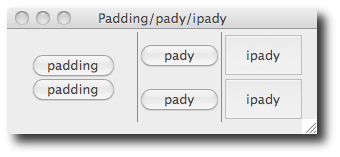
\includegraphics[width=.6\textwidth]{fig-tcltk-padding-pady-ipady}
  \caption{Various ways to put padding between widgets using
    \function{tkpack}. The \code{padding} option for the box container
    puts padding around the cavity for all the widgets. The
    \code{pady} option for \function{tkpack} puts padding around the
    top and bottom on the border of each widget. The \code{ipady}
    option for \function{tkpack} puts padding within the top and
    bottom of the border for each child (breaking the theme under Mac
    OS X).}
  \label{fig:fig-pack-example}
\end{figure}


\ilayout{spacing}
In addition to the \code{padding} option for a frame container, the
\option{ipadx}{tkpack}, \option{ipady}{tkpack}, \option{padx}{tkpack},
and \option{pady}{tkpack} options can be used to add space around the
child components. Figure~\ref{fig:fig-pack-example} has an
example. In the above options, the \code{x} and \code{y} indicate left-right space or
top-bottom space. The \code{i} stands for internal padding that is
left on the sides or top and bottom of the child within the border,
for \code{padx} the external padding added around the border of the
child component. The value can be a single number or pair of numbers
for asymmetric padding.


This sample code shows how one can easily add padding around all the
children of the frame \code{f} using the
\subcommand{"configure"}{tkpack} subcommand.

\begin{Schunk}
\begin{Sinput}
 allChildren <- as.character(tkwinfo("children", f))
 sapply(allChildren, tkpack.configure,  padx=10, pady=5)
 
\end{Sinput}
\end{Schunk}


\paragraph{Cavity model}
The packing algorithm, as described in the \Tk\/ documentation, is based
on arranging where to place a slave into the rectangular unallocated
space called a ``cavity.'' We use the nicer terms ``child component'' and ``box''
to describe these. When a child is placed inside the box, say on the
top, the space allocated to the child is the rectangular space with
width given by the width of the box, and height the sum of the
requested height of the child plus twice the \code{ipady} amount (or
the sum if specified with two numbers). The packer then chooses the
dimension of the child component, again from the requested size plus
the \code{ipad} values for \code{x} and \code{y}. These two spaces
may, of course, have different dimensions.



By default, the child  will be placed centered along the edge of
the box within the allocated space and blank space, if any, on both
sides. 


%% has a thorough explanation: http://www.rigacci.org/docs/biblio/online/lperltk/ch02.html
\paragraph{The anchor, expand, fill arguments}\ilayout{alignment}
When there is more space in the box than requested by the child
component, there are other options. The \option{anchor}{tkpack} option
can be used to anchor the child to a place in the box by specifying
one of the valid compass points (eg. \code{"n"} or \code{"se"})
leaving blank space around the child (Figure~\ref{fig:fig-tcltk-anchor-compass}.)

\begin{figure}
  \centering
  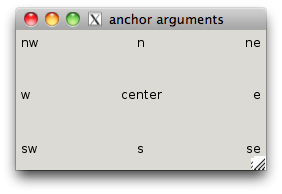
\includegraphics[width=.5\textwidth]{fig-tcltk-anchor-compass.png}
  \caption{The \code{anchor} argument is specified through compass directions}
  \label{fig:fig-tcltk-anchor-compass}
\end{figure}


An alternative is to have one or more of the widgets expand to fill
the available space. Each child packed in with the 
option \option{expand}{tkpack} set to \code{TRUE} will have
the extra space allocated  to it in an even manner. The
\option{fill}{tkpack} option is used to base the size of the child on
the available cavity in the box -- not on the requested size of the
child. The \code{fill} option can be \qcode{x}, \qcode{y} or
\qcode{both}. The first two expanding the child's size in just one
direction, the latter in both.

\begin{example}{Expand/fill options for \function{tkpack}}{eg-tcltk-tkpack-options}
%
\begin{figure}
  \centering
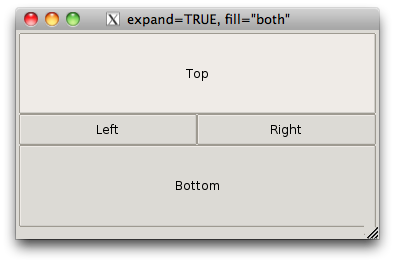
\includegraphics[width=.4\textwidth]{fig-tcltk-expand-fill-both.png}
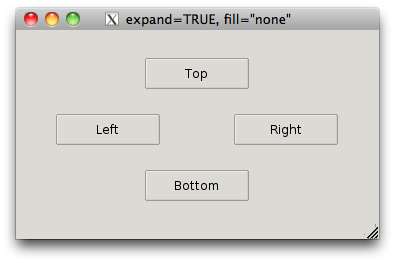
\includegraphics[width=.4\textwidth]{fig-tcltk-expand-fill-none.png}\\
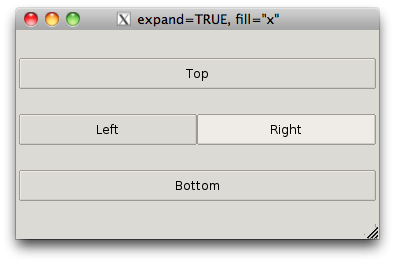
\includegraphics[width=.4\textwidth]{fig-tcltk-expand-fill-x.png}
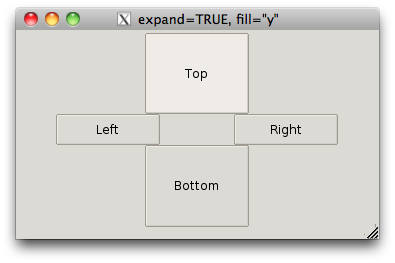
\includegraphics[width=.4\textwidth]{fig-tcltk-expand-fill-y.png}
 \caption{Similar layout with \code{expand=TRUE} but different values
   of \code{fill}. The space allocated to the  top and bottom buttons
   through expansion fills the vertical area, as these were added with
   \code{side="top"} and \code{side="bottom"}; whereas the left and
   right buttons expand in the horizontal direction, as they were
   added with sides \code{left} and \code{right}. The different
   \code{fill} values direct the buttons to take up this allocated
   space in different manners.}
 \label{fig:tcltk-expand-fill-arguments}
\end{figure}
%%
%%
Figure~\ref{fig:tcltk-expand-fill-arguments} shows examples of
different values for \qcode{fill} when \code{expand=TRUE} is
specified. Following an example of Walsh\footcite{Walsh} we used the following code to create the
images:
\begin{Schunk}
\begin{Sinput}
 w <- tktoplevel()
 tkwm.title(w, "Expand/Fill arguments")
 f <- ttkframe(w, padding=c(3,3,12,12))
 tkpack(f, expand=TRUE, fill="both")
 ##
 packButton <- function(txt, ...) 
   tkpack(b <- ttkbutton(f, text=txt), ...)
 ##
 packButton("Top",    side="top",    expand=TRUE, fill="both") 
 packButton("Bottom", side="bottom", expand=TRUE, fill="both") 
 packButton("Left",   side="left",   expand=TRUE, fill="both") 
 packButton("Right",  side="right",  expand=TRUE, fill="both") 
\end{Sinput}
\end{Schunk}
%

Modifying the fill styles was easy, for example
\begin{Schunk}
\begin{Sinput}
 children <- as.character(tkwinfo("children", f))
 sapply(children, tkpack.configure, fill="none")
\end{Sinput}
\end{Schunk}
\end{example}



\paragraph{Not enough space}
When the toplevel window does not have sufficient space to satisfy the
combined size requests of its child components either some
widgets will be covered or one can resize the toplevel window.
When components are covered, the ones that are packed in first are given
highest priority in the size request.

To force a recomputation of of the size of the toplevel window, one can
call the \subcommand{geometry}{wm} subcommand with an empty string:
\begin{Schunk}
\begin{Sinput}
 tkwm.geometry(tt, "")
\end{Sinput}
\end{Schunk}
%
The toplevel window, \code{tt} above, can be recovered from a child
component, say \code{b}, through
\begin{Schunk}
\begin{Sinput}
 tkwinfo("toplevel", b)
\end{Sinput}
\end{Schunk}


%


\paragraph{propagate}
In Example~\ref{ex-tcltk-populate-treeview} we define a convenience
function for creating a table widget. There we have a call to the
subcommand \subcommand{propagate}{pack}.  This prevents the querying
of the child widgets to compute the size request. In the example, this
is useful as the scrollbars used should depend on the size requested
by the parent, and not the underlying table widget.


\begin{example}{Packing dialog buttons}{ex-tcltk-pack}
%%
%%
This example shows how one can pack in action buttons, such as when a
dialog is created.

\begin{figure}
  \centering
  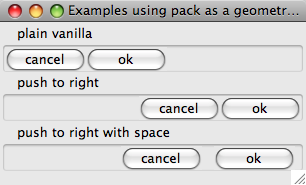
\includegraphics[width=.5\textwidth]{fig-tcltk-pack-buttons.png}
  \caption{Demonstration of using \code{tkpack} options showing
    effects of using the \code{side}
    and \code{padx} options to create
    dialog buttons.}
  \label{fig:tcltk-pack-buttons}
\end{figure}


The first example just uses \code{tkpack} without any arguments except
the side to indicate the buttons are packed in left to right, not top
to bottom.
\begin{Schunk}
\begin{Sinput}
 f1 <- ttklabelframe(f, text="plain vanilla")
 tkpack(f1, expand=TRUE, fill="x")
 l <- function(f) 
   list(ttkbutton(f, text="cancel"), ttkbutton(f, text="ok"))
 sapply(l(f1), tkpack, side="left")
\end{Sinput}
\end{Schunk}

Typically the buttons are right justified. One way to do this is to
pack in using \code{side} with a value of \qcode{right}. This shows
how to use a blank expanding label to take up the space on the left.\ilayout{spring}
\begin{Schunk}
\begin{Sinput}
 f2 <- ttklabelframe(f, text="push to right")
 tkpack(f2, expand=TRUE, fill="x")
 tkpack(ttklabel(f2, text=" "), 
        expand=TRUE, fill="x", side="left")
 sapply(l(f2), tkpack, side="left")
\end{Sinput}
\end{Schunk}

Finally, we add in some padding to conform to Apple's design specification that such
buttons should have a 12 pixel separation.
\begin{Schunk}
\begin{Sinput}
 f3 <- ttklabelframe(f, text="push to right with space")
 tkpack(f3, expand=TRUE, fill="x")
 tkpack(ttklabel(f3, text=" "), expand=TRUE, fill="x", 
        side="left")
 sapply(l(f3), tkpack, side="left", padx=6)
\end{Sinput}
\end{Schunk}
\end{example}

\begin{example}{A non-modal dialog}{ex-tcltk-non-modal-dialog}
This example shows how to use  a window, frames,  labels, buttons,
icons, packing and bindings to create a non-modal dialog. 

\begin{figure}
  \centering
  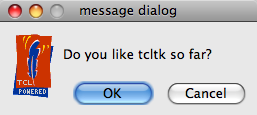
\includegraphics[width=.4\textwidth]{fig-tcltk-simple-dialog.png}
  \caption{Example of a simple dialog}
  \label{fig:fig-tcltk-simple-dialog}
\end{figure}

Although not written as a function, we set aside the values that would
be passed in were it.
\begin{Schunk}
\begin{Sinput}
 title <- "message dialog"
 message <- "Do you like tcltk so far?"
 parent <- NULL
 tkimage.create("photo", "::img::tclLogo", 
                file = system.file("images","tclp.gif",
                  package="ProgGUIinR"))
\end{Sinput}
\end{Schunk}

The main top-level window is given a title, then withdrawn while
the GUI is created. 
\begin{Schunk}
\begin{Sinput}
 w <- tktoplevel(); tkwm.title(w, title)
 tkwm.state(w, "withdrawn")
 f <- ttkframe(w,  padding=c(3, 3, 12, 12))
 tkpack(f, expand=TRUE, fill="both")
\end{Sinput}
\end{Schunk}
As usual, we added a frame so that any themes are respected.

If the parent is non-null and is viewable, then the dialog is made
transient to a parent, The parent need not be a top-level window, so
\function{tkwinfo} if used to find the parent's top-level window. For
Mac OS X, we use the \code{notify} attribute to bounce the dock icon
until the mouse enters the window area.

\begin{Schunk}
\begin{Sinput}
 if(!is.null(parent)) {
   parentWin <- tkwinfo("toplevel", parent)
   if(as.logical(tkwinfo("viewable", parentWin))) {
     tkwm.transient(w, parent)
     if(as.character(tcl("tk", "windowingsystem")) == "aqua") {
       tcl("wm","attributes",parentWin, notify=TRUE) # bounce
       tkbind(parentWin,"<Enter>", function()        # stop
              tcl("wm","attributes",parentWin, notify=FALSE)) 
     }
   }
 }
\end{Sinput}
\end{Schunk}

We will use a standard layout for our dialog with an icon on the left,
a message and buttons on the right. We pack the icon into the left side of the frame,
\begin{Schunk}
\begin{Sinput}
 l <- ttklabel(f, image="::img::tclLogo", padding=5) # recycle
 tkpack(l,side="left")
\end{Sinput}
\end{Schunk}

A nested frame will be used to layout the message area and button area. Since the \function{tkpack} default is to pack in top to bottom, no \code{side} specification is made.
\begin{Schunk}
\begin{Sinput}
 f1 <- ttkframe(f)
 tkpack(f1, expand=TRUE, fill="both")
 #
 m <- ttklabel(f1, text=message)
 tkpack(m, expand=TRUE, fill="both")
\end{Sinput}
\end{Schunk}

The buttons have their own frame, as they are layed out horizontally. 
\begin{Schunk}
\begin{Sinput}
 f2 <- ttkframe(f1)
 tkpack(f2)
\end{Sinput}
\end{Schunk}
%
The callback function for the OK button prints a message then destroys the window.
\begin{Schunk}
\begin{Sinput}
 okCB <- function() {
   print("That's great")
   tkdestroy(w)
 }
 okButton <- ttkbutton(f2, text="OK", command=okCB)
 cancelButton <- ttkbutton(f2, text="Cancel", 
                           command=function() tkdestroy(w))
 #
 tkpack(okButton, side="left", padx=12)  # give some space
 tkpack(cancelButton)
\end{Sinput}
\end{Schunk}
%

As our interactive behavior is consistent for both buttons, we make a
binding to the \code{TButton} class, not individually. The first will
invoke the button command when the \kbd{return} key is pressed, the
latter two will highlight a button when the focus is on it.
\begin{Schunk}
\begin{Sinput}
 tkbind("TButton", "<Return>", function(W) tcl(W, "invoke"))
 tkbind("TButton", "<FocusIn>", function(W) 
        tcl(W, "state", "active"))
 tkbind("TButton", "<FocusOut>", function(W) 
        tcl(W, "state", "!active"))
\end{Sinput}
\end{Schunk}
%
Now we bring the dialog back from its withdrawn state, fix the size
and set the initial focus on the OK button.
\begin{Schunk}
\begin{Sinput}
 tkwm.state(w, "normal")
 tkwm.resizable(w, FALSE, FALSE)
 tkfocus(okButton)
\end{Sinput}
\end{Schunk}
\end{example}


\subsection{Grid}
\label{sec:tcltk:grid}
\ilayout{grid layout}
The \function{tkgrid} geometry manager is used to align child widgets
in rows and columns.  In its simplest usage, a command like
\begin{Schunk}
  \begin{Sinput}
tkgrid(child1, child2,..., childn)    
  \end{Sinput}
\end{Schunk}
will place the $n$ children in a new row, in columns $1$ through
$n$. If desired, the specific row and column can be specified through the
\option{row}{tkgrid} and \option{column}{tkgrid} options, counting of
rows and columns starts with $0$.  Spanning of multiple rows and columns
can be specified with integers $2$ or greater by the
\option{rowspan}{tkgrid} and \option{colspan}{tkgrid} options. These
options, and others, can be adjusted through the
\function{tkgrid.configure} function.


\paragraph{The \code{tkgrid.rowconfigure} and \code{tkgrid.columnconfigure} commands}
When the managed container is resized, the grid manager consults
weights that are assigned to each row and column to see how to
allocate the extra space. Allocation is based on proportions, not
specified sizes. The weights are configured with the
\index{tkgrid!\code{rowconfigure}}\function{tkgrid.rowconfigure} and \function{tkgrid.columnconfigure}
functions through the option \option{weight}{tkgrid.columnconfigure}.
The weight is a value between $0$ and $1$. If there are just two rows, and
the first row has weight $1/2$ and the second weight $1$, then the extra
space is allocated twice as much for the second row. The specific row
or column must also be specified. Again. rows and columns are referenced
starting with $0$ not the usual \R-like $1$. To specify a weight of $1$
to the first row would be done with a command like:

%
\begin{Schunk}
\begin{Sinput}
 tkgrid.rowconfigure(parent, 0, weight=1)
\end{Sinput}
\end{Schunk}
%
\paragraph{The sticky option}
The \function{tkpack} command had options \code{anchor} and
\code{expand} and \code{fill} to control what happens when more space
is available then requested by a child component. The
\option{sticky}{tkgrid} option for \function{tkgrid} combines
these. The value is a combination of the compass points
\qcode{n},\qcode{e},\qcode{w}, and \qcode{s}. A specification
\qcode{ns} will make the child component ``stick'' to the top and
bottom of the cavity that is provided, similar to the \code{fill="y"}
option for \function{tkpack}. A value of \qcode{news} will make the
child component expand in all the direction like \code{expand=TRUE, fill="both"}.

\paragraph{Padding}
As with \function{tkpack}, \function{tkgrid} has options
\option{ipadx}{tkgrid}, \option{ipady}{tkgrid}, \option{padx}{tkgrid},
and \option{padx}{tkgrid} to give internal and external space around a
child.

\paragraph{Size}
The function \function{tkgrid.size} will return the number of columns
and rows of the specified parent container that is managed by a
grid. This can be useful when trying to position child components
through the options \code{row} and \code{column}.

\paragraph{Forget}
To remove a child from the parent, the \function{tkgrid.forget}
function can be used with the child object as its argument.


% \begin{example}{Using \function{tkgrid} and \function{tkpack} to draw some world flags}{ex-tcltk-flags}
%   \SweaveInput{ex-tcltk-flags.Rnw}
% \end{example}


\begin{example}{Using \function{tkgrid} to create a toolbar}{ex-tcltk-toolbar}
%
\begin{figure}
  \centering
  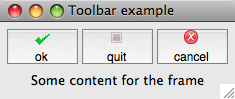
\includegraphics[width=.6\textwidth]{fig-tcltk-toolbar.png}
  \caption{Illustration of using \code{tkpack} and \code{tkgrid} to make a toolbar. }
  \label{fig:fig-tcltk-toolbar}
\end{figure}
%%
\TK\/ does not have a toolbar widget. Here we use \function{tkgrid} to
show how we can add one to a top-level window in a manner that is not
affected by resizing. We begin by packing a frame into a
top-level window.
\begin{Schunk}
\begin{Sinput}
 w <- tktoplevel(); tkwm.title(w, "Toolbar example")
 f <- ttkframe(w, padding=c(3,3,12,12))
 tkpack(f, expand=TRUE, fill="both")
\end{Sinput}
\end{Schunk}
Our example has two main containers: one to hold the toolbar buttons
and one to hold the main content.
\begin{Schunk}
\begin{Sinput}
 tbFrame <- ttkframe(f, padding=0)
 contentFrame <- ttkframe(f, padding=4)
\end{Sinput}
\end{Schunk}
The \function{tkgrid} geometry manager is used to place the toolbar at
the top, and the content frame below. The choice of sticky and the weights ensure that
the toolbar does not resize if the window does.
\begin{Schunk}
\begin{Sinput}
 tkgrid(tbFrame, row=0, column=0, sticky="we")
 tkgrid(contentFrame, row=1, column=0, sticky = "news")
 tkgrid.rowconfigure(f, 0, weight=0)
 tkgrid.rowconfigure(f, 1, weight=1)
 tkgrid.columnconfigure(f, 0, weight=1)
 #
 txt <- "Lorem ipsum dolor sit amet..." # sample text
 tkpack(ttklabel(contentFrame, text=txt))
\end{Sinput}
\end{Schunk}

Now to add some buttons to the toolbar. We first show how to create a
new style for a button (\code{Toolbar.TButton}), slightly modifying the themed button to set
the font and padding, and eliminate the border if the operating system allows. 
\begin{Schunk}
\begin{Sinput}
 tcl("ttk::style", "configure", "Toolbar.TButton", 
     font="helvetica 12", padding=0, borderwidth=0)
\end{Sinput}
\end{Schunk}
%
This \code{makeIcon} function finds stock icons from the
\pkg{gWidgets} package and adds them to a button.
\begin{Schunk}
\begin{Sinput}
 makeIcon <- function(parent, stockName, command=NULL) {
   iconFile <- system.file("images", 
                           paste(stockName,"gif",sep="."), 
                           package="gWidgets")
   if(nchar(iconFile) == 0) {
     b <- ttkbutton(parent, text=stockName, width=6)
   } else {
     iconName <- paste("::img::",stockName, sep="")
     tkimage.create("photo", iconName, file = iconFile)
     b <- ttkbutton(parent, image=iconName, 
                    style="Toolbar.TButton", text=stockName, 
                    compound="top", width=6)
     if(!is.null(command))
       tkconfigure(b, command=command)
   }
   return(b)
 }
\end{Sinput}
\end{Schunk}
%
To illustrate, we pack in some icons. Here we use \function{tkpack}.  
One does not use \function{tkpack} and \function{tkgrid} to manage
children of the same parent, but these are children of \code{tbFrame},
not \code{f}.
\begin{Schunk}
\begin{Sinput}
 sapply(c("ok", "quit", "cancel"), function(i)
        tkpack(makeIcon(tbFrame, i), side="left"))
\end{Sinput}
\end{Schunk}

These two bindings change the state of the buttons as the mouse hovers
over it:

\begin{Schunk}
\begin{Sinput}
 setState <- function(W, state) tcl(W, "state", state)
 tkbind("TButton", "<Enter>", function(W) setState(W, "active"))
 tkbind("TButton", "<Leave>", function(W) setState(W, "!active"))
\end{Sinput}
\end{Schunk}

If one wished to restrict the above to just the toolbar buttons, one
could check for the style of the button, as with:

\begin{Schunk}
\begin{Sinput}
 function(W) {
   if(as.character(tkcget(W, "-style")) == "Toolbar.TButton")
     cat("... do something for toolbar buttons ...")
 }
\end{Sinput}
\end{Schunk}
\end{example}

\begin{example}{Using \function{tkgrid} to layout a calendar}{ex-tkgrid-calendar}
This example shows how to create a simple calendar using a grid
layout. (No such widget is standard with \pkg{tcltk}.) We use some
data functions for the \pkg{ProgGUIinR} package. The actual use of
\function{tkgrid} is straightforward once the approporiate row and
column is figured out.




\begin{figure}
  \centering
  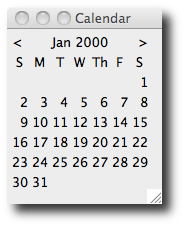
\includegraphics[width=.35\textwidth]{fig-tcltk-grid-calendar}
  \caption{A monthly calendar illustrating various layouts.}
  \label{fig:qt-gridlayout-calendar}
\end{figure}


\begin{Schunk}
\begin{Sinput}
 makeMonth <- function(w, year, month) {
   ## add headers
   days <- c("S","M","T","W","Th","F","S")
   sapply(1:7, function(i) {
     l <- ttklabel(w, text=days[i])       
     tkgrid(l, row=0, column=i-1, sticky="")
   })
   ## add days
   sapply(seq_len(ProgGUIinR:::days.in.month(year, month)), 
          function(day) {
            l <- ttklabel(w, text=day)
            row <- ProgGUIinR:::week.of.month(year, month, day)
            col <- ProgGUIinR:::day.of.week(year, month, day)
            tkgrid(l, row=1 + row, column=col, sticky="e")
          })
 }
\end{Sinput}
\end{Schunk}

Next, we would like to incorporate the calendar widget into an interface
that allows the user to scroll through month-by-month beginning with:
\begin{Schunk}
\begin{Sinput}
 year <- 2000; month <- 1
\end{Sinput}
\end{Schunk}

Our basic layout will use a box layout with a nested layout
for the step-through controls and another holding the calendar widget.
\begin{Schunk}
\begin{Sinput}
 w <- tktoplevel()
 f <- ttkframe(w, padding=c(3,3,12,12))
 tkpack(f, expand=TRUE, fill="both", side="top")
 cframe <- ttkframe(f)
 calframe <- ttkframe(f)
 tkpack(cframe, fill="x", side="top")
 tkpack(calframe, expand=TRUE, anchor="n")
\end{Sinput}
\end{Schunk}

Our step through controls are packed in through a horizontal
layout. We use anchoring and \code{expand=TRUE} to keep the arrows on the edge and the
label with the current month centered, should the container be resized.
\begin{Schunk}
\begin{Sinput}
 prevb <- ttklabel(cframe, text="<")
 nextb <- ttklabel(cframe, text=">")
 curmo <- ttklabel(cframe)
 #
 tkpack(prevb, side="left", anchor="w")
 tkpack(curmo, side="left", anchor="center", expand=TRUE)
 tkpack(nextb, side="left", anchor="e")
\end{Sinput}
\end{Schunk}

The \code{setMonth} function first removes the previous calendar
container and then
redefines one to hold the monthly calendar. Then it adds in a new
monthly calendar to match the year and month. The call to
\code{makeMonth} creates the calendar. Packing in the frame after
adding its child components makes the GUI seem much more responsive.
\begin{Schunk}
\begin{Sinput}
 setMonth <- function() {
   tkpack("forget", calframe)
   calframe <<- ttkframe(f)
   makeMonth(calframe, year, month)
   tkconfigure(curmo,                    # month label
               text=sprintf("%s %s", month.abb[month], year))
   tkpack(calframe)
 }
 setMonth()                              # initial calendar
\end{Sinput}
\end{Schunk}

The arrow labels are used to scroll, so we connect to the
\event{Button-1} event the corresponding commands. This shows the
binding to decrement the month and year using the global variables
\code{month} and \code{year}.
\begin{Schunk}
\begin{Sinput}
 tkbind(prevb, "<Button-1>", function() {
   if(month > 1) {
     month <<- month - 1
   } else {
     month <<- 12; year <<- year - 1
   }
   setMonth()
 })
\end{Sinput}
\end{Schunk}


Our calendar is static, but if we wanted to add interactivity to a
mouse click, we could make a binding as follows:
  
\begin{Schunk}
\begin{Sinput}
 tkbind("TLabel", "<Button-1>", function(W) {
   day <- as.numeric(tkcget(W, "-text"))
   if(!is.na(day))
     print(sprintf("You selected: %s/%s/%s", month, day, year))
 })
\end{Sinput}
\end{Schunk}


\end{example}

\section{Other containers}
\label{sec:tcltk:other-containers}
\TK\/ provides just a few other basic containers, here we describe paned windows and notebooks.

\subsection{Paned windows}
\label{sec:tcltk:paned-windows}

A paned window, with sashes to control the individual pane sizes, is constructed by the function
\constructor{ttkpanedwindow}. The primary option, outside of setting
the requested width or height with \option{width}{ttkpanedwindow} and
\option{height}{ttkpanedwindow}, is \option{orient}{ttkpanedwindow},
which takes a value of \qcode{vertical} (the default) or
\qcode{horizontal}. This specifies how the children are stacked, and
is opposite of how the sash is drawn.

%% adding
The returned object can be used as a parent container, although one
does not use the geometry managers to manage them. Instead, the
\method{add}{ttkpanedwindow} command is used to add a child component. For example:
\begin{Schunk}
\begin{Sinput}
 w <- tktoplevel(); tkwm.title(w, "Paned window example")
 pw <- ttkpanedwindow(w, orient="horizontal")
 tkpack(pw, expand=TRUE, fill="both")
 left <- ttklabel(pw, text="left")
 right <- ttklabel(pw, text="right")
 #
 tkadd(pw, left, weight=1)
 tkadd(pw, right, weight=2)
\end{Sinput}
\end{Schunk}
%
When resizing which child gets the space is determined by the
associated \code{weight}, specified as an integer. The default uses
even weights.  Unlike \GTK\/ more than two children are allowed.

\paragraph{Forget}
The subcommand \subcommand{forget}{ttkpanedwindow} can be used to
unmanage a child component. For the paned window, we have no
convenience function, so we call as follows:
\begin{Schunk}
\begin{Sinput}
 tcl(pw, "forget", right)
 tkadd(pw, right, weight=2) ## how to add back
\end{Sinput}
\end{Schunk}
%
\paragraph{Sash position}
The sash between two children can be adjusted through the subcommand
\subcommand{sashpos}{ttkpanedwindow}. The index of the sash needs
specifying, as there can be more than one. Counting starts at 0. The
value for \code{sashpos} is in terms of pixel width (or height) of the
paned window. The width can be returned and used as follows:
\begin{Schunk}
\begin{Sinput}
 width <- as.integer(tkwinfo("width", pw))  # or "height"
 tcl(pw, "sashpos", 0, floor(0.75*width))
\end{Sinput}
\begin{Soutput}
<Tcl> 54 
\end{Soutput}
\end{Schunk}
%

\subsection{Notebooks}
\label{sec:tcltk:notebooks}

%% constructor

%
\begin{figure}
  \centering
  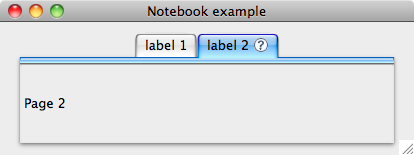
\includegraphics[width=.6\textwidth]{fig-tcltk-notebook}
 \caption{A basic notebook under \OSX{}}
  \label{fig:fig-notebook-example}
\end{figure}

Tabbed notebook containers are produced by the
\constructor{ttknotebook} constructor.  Notebook pages can be added
through the \subcommand{add}{ttknotebook} subcommand or inserted after
a page through the \subcommand{insert}{ttknotebook} subcommand. The
latter requires a tab ID to be specified, as described below.
Typically, the child components would be containers to hold more
complicated layouts. The tab label is configured similarly to
\function{ttklabel} through the options \option{text}{ttknotebook} and
(the optional) \option{image}{ttknotebook}, which if given has its
placement determined by \option{compound}{ttknotebook}.  The placement
of the child component within the notebook page is manipulated
similarly as \function{tkgrid} through the
\option{sticky}{ttknotebook} option with values specified through
compass points. Extra padding around the child can be added with the
\option{padding}{ttknotebook} option.

\paragraph{Tab identifiers} %%integer (0-based), object (ID), "current", "end"
Many of the commands for a notebook require a specification of a
desired tab. This can be given by index, starting at 0; by the values
\code{"current"} or \code{"end"}; by the child object added to the
tab, either as an \R\/ object or an ID; or in terms of $x$-$y$
coordinates in the form \code{"@x,y"} (likely found through a
binding).

%% illustrate add, inser
To illustrate, if \code{nb} is a \code{ttknotebook} object, then these
commands would add pages (cf. Figure~\ref{fig:fig-notebook-example}):
\begin{Schunk}
\begin{Sinput}
 iconFile <- system.file("images",paste("help","gif",sep="."),
                         package="gWidgets")
 iconName <- "::tcl::helpIcon"
 tkimage.create("photo", iconName, file = iconFile)
 #
 l2 <- ttklabel(nb, text="Page 2")
 tkadd(nb, l2, sticky="nswe", text="label 2", 
     image=iconName, compound="right")
 ## put l1 first (a tabID of 0); use tkinsert
 l1 <- ttklabel(nb, text="Page 1")
 tkinsert(nb, 0, l1, sticky="nswe", text="label 1")
\end{Sinput}
\end{Schunk}
%
There are several useful subcommands to extract information from the
notebook object.  For instance, \code{index} to return the page index
(0-based), \code{tabs} to return the page IDs, \code{select} to select
the displayed page, and \code{forget} to remove a page from the
notebook. (There is no means to place close icons on the tabs.)
Except for \code{tabs}, these require a specification of a tab ID.
\begin{Schunk}
\begin{Sinput}
 tcl(nb, "index", "current")           # current page for tabID
\end{Sinput}
\begin{Soutput}
<Tcl> 1 
\end{Soutput}
\begin{Sinput}
 length(as.character(tcl(nb,"tabs")))  # number of pages
\end{Sinput}
\begin{Soutput}
[1] 2
\end{Soutput}
\begin{Sinput}
 tcl(nb, "select", 0)        # select viewable page by index
 tcl(nb, "forget", l1)       # "forget" removes a page
 tcl(nb, "add", l1)          # can be managed again.
\end{Sinput}
\end{Schunk}
%

%% keyboard
The notebook state can be manipulated through the keyboard, provided traversal is enabled. This can be done through
\begin{Schunk}
\begin{Sinput}
 tcl("ttk::notebook::enableTraversal", nb)
\end{Sinput}
\end{Schunk}

If enabled, the shortcuts such as \kbd{control-tab} to move to the
next tab are implemented. If new pages are added or inserted with the
option \option{underline}{ttknotebook}, which takes an integer value
(0-based) specifying which character in the label is underlined, then
a keyboard accelerator is added for that letter.

\paragraph{Bindings}
%% virtualevent
Beyond the usual events, the notebook widget also generates a
\code{\VirtualEvent{NotebookTabChanged}} virtual event after a new tab is
selected.

%% limitations: no easy way to get close buttons (to me anyways); no
%% graceful way to handle too man tabs.
The notebook container in \TK\/ has a few limitations. For instance,
there is no graceful management of too many tabs, as there is with
\GTK, as well there is no easy way to implement close buttons as an
icon, as in \Qt.


\chapter{Tcl/Tk: Dialogs and Widgets}
\label{sec:tcltk:widgets}

This chapter covers both the standard dialogs provided by \TK\/ and
the various controls used to create custom dialogs. We begin with a
discussion of these standard dialogs, then cover the basic controls
in this chapter, leaving the next chapter for the more involved \constructor{tktext},
\constructor{ttktreeview}, and \constructor{tkcanvas} widgets.

%% Rewrite
% \Tk\/ has widgets for the common GUI controls. As mentioned in
% Chapter~\ref{sec:tcltk:overview} -- where we illustrated both buttons
% and labels -- the constructors for these widgets call the function
% \function{tkwidget} which calls the appropriate \TK\/ command and adds
% in extra information including an ID and an environment. As with
% labels and buttons, one primarily uses \function{tkconfigure} and
% \function{tkcget} to set and get properties of the widget when a
% \TCL\/ variable is not used to store the data for the widget.



\section{Dialogs}
\label{sec:tcltk:dialogs}
\subsection{Modal dialogs}
\label{sec:modal-dialogs}

\begin{figure}
  \centering
  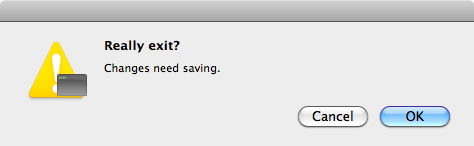
\includegraphics[width=.6\textwidth]{fig-tcltk-confirm-dialog.png}
  \caption{A basic modal dialog constructed by \code{tkmessageBox}.}
  \label{fig:fig-tcltk-confirm-dialog}
\end{figure}

%% messageBox
\igui{modal dialog}
The \constructor{tkmessageBox} constructor can be used to create
simple modal dialogs allowing a user to confirm an action, using the
native toolkit if possible. This constructor replaces the older
\code{tkdialog} dialogs. The arguments \argument{title}{tkmessageBox},
\argument{message}{tkmessageBox} and \argument{detail}{tkmessageBox}
are used to set the text for the dialog. The \code{title} may not
appear for all operating systems. A messageBox dialog has an
\argument{icon}{tkmessageBox} argument. The default icon is
\qcode{info} but could also be one of \qcode{error}, \qcode{question},
or \qcode{warning}. The buttons used are specified through the
\argument{type}{tkmessageBox} argument with values of \qcode{ok},
\qcode{okcancel}, \qcode{retrycancel}, \qcode{yesno}, or
\qcode{yesnocancel}. When a button is clicked the dialog is destroyed
and the button label returned as a value. The argument
\argument{parent}{tkmessageBox} can be given to specify which window
the dialog belongs to. Depending on the operating system this may be
used when drawing the dialog.

A sample usage is:
\begin{Schunk}
\begin{Sinput}
 tkmessageBox(title="Confirm", message="Really exit?", 
              detail="Changes need saving.", 
              icon="question", type="okcancel")
\end{Sinput}
\end{Schunk}
%% 

\paragraph{The tkwait function}
If the default modal dialog is not enough -- for instance there is no
means to gather user input -- then a toplevel window can be made
modal. The \function{tkwait} function will cause a top-level window to
be modal and \function{tkgrab.release} will return the interactivity
for the window. We illustrate a simple use by example, beginning by
adding a label to a window:

\begin{Schunk}
\begin{Sinput}
 message <- "We care ..."
 dlg <- tktoplevel(); tkwm.withdraw(dlg)
 tkwm.overrideredirect(dlg, TRUE)   # no decoration
 f <- ttkframe(dlg, padding=5)
 tkpack(f, expand=TRUE, fill="both")
 tkpack(ttklabel(f, text=message), pady=5)
\end{Sinput}
\end{Schunk}

There a different ways to use \code{tkwait}. The function
\function{tkwait.window} will make a toplevel window modal waiting
until it is destroyed. In the following we use
\function{tkwait.variable}, which waits for a change to a variable, in
this case \code{flag}.  In the button's command we release the window
then change this value, ending the wait.
\begin{Schunk}
\begin{Sinput}
 flag <- tclVar("")
 tkpack(ttkbutton(f, text="dismiss", command=function() {
   tkgrab.release(dlg)
   tclvalue(flag) <- "Destroy"
 }))
\end{Sinput}
\end{Schunk}
Now we show the window and wait on the \code{flag} variable to change.
\begin{Schunk}
\begin{Sinput}
 tkwm.deiconify(dlg)
 tkwait.variable(flag)
\end{Sinput}
\end{Schunk}

When the flag is changed, the flow returns to the program. Here we
print a message then destroy the dialog.
\begin{Schunk}
\begin{Sinput}
 print("Thanks")
\end{Sinput}
\begin{Soutput}
[1] "Thanks"
\end{Soutput}
\begin{Sinput}
 tkdestroy(dlg)
\end{Sinput}
\end{Schunk}


\subsection{File and directory selection}
\label{sec:file-direct-select}

\Tk\/ provides constructors for selecting a file, for selecting a
directory or for specifying a filename when saving. These are
implemented by \constructor{tkgetOpenFile},
\constructor{tkchooseDirectory}, and \constructor{tkgetSaveFile}
respectively. Each of these can be called with no argument, and
each returns a \code{tclObj} object. The value is empty when there is no selection made.

The dialog will appear in a relationship with a toplevel window if the argument
\argument{parent}{tkgetOpenFile} is specified The
\argument{initialdir}{tkgetOpenFile} and
\argument{initialfile}{tkgetOpenFile} can be used to specify the
initial values in the dialog.  The
\argument{defaultextension}{tkgetSaveFile} argument can be used to
specify a default extension for the file.

When browsing for files, it can be convenient to filter the available
file types that can be selected. The \argument{filetypes}{tkgetOpenFile} argument is used for this task. However,
the file types are specified using \TCL\/ brace-notation, not \R\/ code. For example,
to filter out various image types, one could have 
\begin{Schunk}
\begin{Sinput}
 tkgetOpenFile(filetypes = paste(
                 "{{jpeg files} {.jpg .jpeg} }",
                 "{{png files} {.png}}",
                 "{{All files} {*}}", sep=" ")) # needs space
\end{Sinput}
\end{Schunk}
Extending this is hopefully clear from the pattern above.

\begin{example}{A ``File'' menu}{ex-tcltk-file-menu}
  To illustrate, a simple example for a file menu (Section~\ref{sec:tcltk:menus}) could include:
\begin{Schunk}
\begin{Sinput}
 w <- tktoplevel(); tkwm.title(w, "File menu example")
 mb <- tkmenu(w); tkconfigure(w, menu=mb)
 fileMenu <- tkmenu(mb)
 tkadd(mb, "cascade", label="File", menu=fileMenu)
 tkadd(fileMenu,"command",label="Source file...",
       command= function() {
         fName <- tkgetOpenFile(filetypes=
                         "{{R files} {.R}} {{All files} *}")
         if(file.exists(fName <- as.character(fName)))
            source(tclvalue(fName))
       })
 tkadd(fileMenu, "command", label="Save workspace as...",
       command=function() {
         fName <- tkgetSaveFile(defaultextension="Rsave")
         if(nchar(fname <- as.character(fName)))
           save.image(file=fName)
       })
 tkadd(fileMenu, "command", label="Set working directory...",
       command=function() {
         dName <- tkchooseDirectory()
         if(nchar(dName <- as.character(dName)))
           setwd(dName)
       })
\end{Sinput}
\end{Schunk}
\end{example}

\subsection{Choosing a color}
\Tk\/ provides the command \code{tk\_chooseColor} to construct a dialog for selection of a color by RGB value. There are three optional arguments \argument{initialcolor}{tk\_chooseColor} to specify an initial color such as \qcode{\#efefef}, \argument{parent}{tk\_chooseColor} to make the dialog a child of a specified window and \argument{title}{tk\_chooseColor} to specify a title for the dialog. The return value is in hex-coded RGB quantities. 
There is no constructor in \pkg{tcltk}, but one can use the dialog as follows:
\begin{Schunk}
\begin{Sinput}
 w <- tktoplevel(); tkwm.title(w, "Select a color")
 f <- ttkframe(w, padding=c(3,3,3,12))
 tkpack(f, expand=TRUE, fill="both")
 colorWell <- tkcanvas(f, width=40, height=16, 
                       background="#ee11aa",
                       highlightbackground="#ababab") 
 tkpack(colorWell)
 tkpack(ttklabel(f, text="Click color to change"))
 #
 tkbind(colorWell,"<Button-1>", function(W) {
   color <- tcl("tk_chooseColor", parent=W, 
                title="Set box color")
   color <- tclvalue(color)
   print(color)
   if(nchar(color))
     tkconfigure(W, background = color)
 })
\end{Sinput}
\end{Schunk}



\section{Selection widgets}
\label{sec:tcltk:selection-widgets}

This section covers the many different ways to present data for the
user to select a value. The widgets can use \TCL\/ variables to refer
to the value that is displayed or that the user selects.  Recall,
these were constructed through \function{tclVar} and manipulated
through \code{tclvalue}.  For example, a logical value can be stored as
\begin{Schunk}
\begin{Sinput}
 value <- tclVar(TRUE)
 tclvalue(value) <- FALSE
 tclvalue(value)
\end{Sinput}
\begin{Soutput}
[1] "0"
\end{Soutput}
\end{Schunk}
As \code{tclvalue} coerces the logical into the  character string  \qcode{0} or \qcode{1}, some coercion may be desired.



\begin{figure}
  \centering
  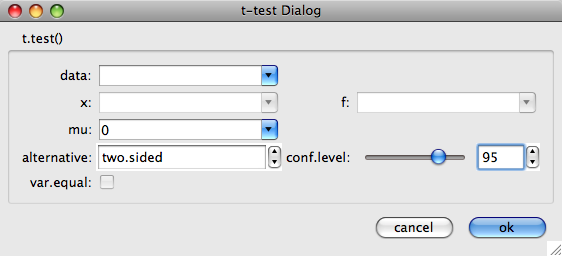
\includegraphics[width=.75\textwidth]{fig-tcltk-t-test.png}
  \caption{A dialog to collect values for a $t$-test (cf.
    Example~\ref{ex-tcltk-t-test}) showing several of the selection
    widgets discussed in the section: a checkbutton, radio button,
    combo boxes, a scale widget and a spinbox.}
  \label{fig:fig-tcltk-t-test}
\end{figure}

\subsection{Checkbutton}
\label{sec:tcltk:checkboxes}

The \constructor{ttkcheckbutton} constructor returns a checkbutton
object. The checkbutton's value (\code{TRUE} or \code{FALSE}) is linked
to a \TCL\/ variable which can be specified using a logical value.
The checkbutton label can also be specified through a \TCL\/ variable
using the \option{textvariable}{ttkcheckbutton} option.  Alternately,
as with the \code{ttklabel} constructor, the label can be specified
through the \option{text}{ttkcheckbutton} option. As well, one can
specify an image and arrange its display -- as is done with
\function{ttklabel} -- using the \option{compound}{ttkcheckbutton}
option.

The \option{command}{ttkcheckbutton} argument is used at construction
time to specify a callback when the button is clicked. The callback is
called when the state toggles, so often a callback considers the state
of the widget before proceeding.  To add a callback with
\function{tkbind} use \code{\Event{ButtonRelease-1}}, as the callback
for the event \code{\Event{Button-1}} is called before the variable is
updated.

For example, if \code{f} is a frame, we can create a new check button
with the following:

\begin{Schunk}
\begin{Sinput}
 value <- tclVar(TRUE)
 callback <- function() print(tclvalue(value))   # uses global
 labelVar <- tclVar("check button label")
 cb <- ttkcheckbutton(f, variable=value, 
                      textvariable=labelVar, command=callback)
 tkpack(cb)
\end{Sinput}
\end{Schunk}


\paragraph{A toggle button}

By default the widget draws with a check box. Optionally the widget
can be drawn as a button, which when depressed indicates a \code{TRUE}
state. This is done by using the style \code{Toolbutton}, as in:
\begin{Schunk}
\begin{Sinput}
 tkconfigure(cb, style="Toolbutton")
\end{Sinput}
\end{Schunk}

The ``Toolbutton'' style in general is for placing widgets into toolbars.


\paragraph{Avoiding global variables}
To avoid using a global variable is not trivial here. There is no easy
way to pass user data through to the callback, and there is no easy
way to get the \R\/ object from the values passed through the \%
substitution values. The variable holding the value can be found
through
\begin{Schunk}
\begin{Sinput}
 tkcget(cb, "variable"=NULL)
\end{Sinput}
\begin{Soutput}
<Tcl> ::RTcl5 
\end{Soutput}
\end{Schunk}

But then, one needs a means to lookup the variable from this id. Here is a
wrapper for the \function{tclVar} function and a lookup function that
use an environment created by the \pkg{tcltk} package in place of a
global variable.

\begin{Schunk}
\begin{Sinput}
 ourTclVar <- function(...) {
   var <- tclVar(...)
   .TkRoot$env[[as.character(var)]] <- var
   var
 }
 ## lookup function
 getTclVarById <- function(id) {
   .TkRoot$env[[as.character(id)]]
 }
\end{Sinput}
\end{Schunk}

Assuming we used \function{ourTclVar} above, then the callback above
could be defined to avoid a (new) global variable by:


\begin{Schunk}
\begin{Sinput}
 callback <- function(W) {
   id <- tkcget(W, "variable"=NULL)
   print(getTclVarById(id))
 }
\end{Sinput}
\end{Schunk}


In Section~\ref{sec:tcltk:scale-widgets} we demonstrate how to encapsulate the widget and its
variable in a reference class so that one need not worry about scoping
rules to reference the variable. 


\subsection{Radio buttons}
\label{sec:tcltk:radio-buttons}

Radiobuttons are basically differently styled checkbuttons linked through a shared \TCL\/
variable. Each radio button is constructed through the
\constructor{ttkradiobutton} constructor. Each button has both a value and
a text label, which need not be the same. The
\option{variable}{ttkradiobutton} option refers to the
value. As with labels, the radio button labels may be specified
through a text variable or the \option{text}{ttkradiobutton} option,
in which case, as with a \code{ttklabel}, an image may also be
incorporated through the \option{image}{ttkradiobutton} and
\option{compound}{ttkradiobutton} options. In \TK\/ the placement of
the buttons is managed by the programmer.


This small example shows how radio buttons could be used for selection
of an alternative hypothesis, assuming \code{f} is a parent container.

\begin{Schunk}
\begin{Sinput}
 values <- c("less", "greater", "two.sided")
 var <- tclVar(values[3])                # initial value
 callback <- function() print(tclvalue(var))
 sapply(values, function(i) {
   rb <- ttkradiobutton(f, variable=var, 
                        text=i, value=i, 
                        command=callback)
   tkpack(rb, side="top", anchor="w")
 })
\end{Sinput}
\end{Schunk}

\subsection{Entry widgets}
\label{sec:tcltk:entry-widgets}

The \constructor{ttkentry} constructor provides a single line text
entry widget. The widget can be associated with a \TCL\/ variable at
construction to facilitate getting and setting the displayed values
through its argument \argument{textvariable}{ttkentry}. The width of
the widget can be adjusted at construction time through the
\argument{width}{ttkentry} argument. This takes a value for the number
of characters to be displayed, assuming average-width characters.  The
text alignment can be set through the \argument{justify}{ttkentry}
argument taking values of \qcode{left} (the default), \qcode{right}
and \qcode{center}. For gathering passwords, the argument
\argument{show}{ttkentry} can be used, such as with
\code{show=}\qcode{*}, to show asterisks in place of all the
characters.

The following constructs a basic example
\begin{Schunk}
\begin{Sinput}
 eVar <- tclVar("initial value")
 e <- ttkentry(w, textvariable=eVar)
 tkpack(e)
\end{Sinput}
\end{Schunk}

We can get and set values using the \TCL\/ variable.
\begin{Schunk}
\begin{Sinput}
 tclvalue(eVar)
\end{Sinput}
\begin{Soutput}
[1] "initial value"
\end{Soutput}
\begin{Sinput}
 tclvalue(eVar) <- "set value"
\end{Sinput}
\end{Schunk}

The \code{get} command can also be used.
\begin{Schunk}
\begin{Sinput}
 tkget(e)
\end{Sinput}
\begin{Soutput}
<Tcl> set value 
\end{Soutput}
\end{Schunk}

\paragraph{Indices}
The entry widget uses an index to record the different positions
within the entry box. This index can be a number (0-based), an
$x$-coordinate of the value (\code{@x}), or one of the values
\qcode{end} and \qcode{insert} to refer to the end of the current text
and the insert point as set through the keyboard or mouse. The mouse
can also be used to make a selection. In this case the indices
\qcode{sel.first} and \qcode{sel.last} describe the selection.

With indices, we can insert  text with the \subcommand{insert}{ttkentry} command
\begin{Schunk}
\begin{Sinput}
 tkinsert(e, "end", "new text")
\end{Sinput}
\end{Schunk}

Or, we can delete a range of text, in this case the first 4
characters, using \subcommand{delete}{ttkentry}:
\begin{Schunk}
\begin{Sinput}
 tkdelete(e, 0, 4)
\end{Sinput}
\end{Schunk}
%
The first value is the left most index to delete (0-based), the second
value the index to the right of the last value deleted.

The \subcommand{icursor}{ttkentry} command can be used to set the
cursor position to the specified index.
\begin{Schunk}
\begin{Sinput}
 tkicursor(e, 0)                         # move to beginning
\end{Sinput}
\end{Schunk}

Finally, we note that the selection can be adjusted using the
\subcommand{selection range}{ttkentry} subcommand. This takes two
indices. Like \code{delete}, the first index specifies the first character of
the selection, the second indicates the character to the right of the
selection boundary. The following example would select all the text.
\begin{Schunk}
\begin{Sinput}
 tkselection.range(e, 0, "end")
\end{Sinput}
\end{Schunk}
The \subcommand{selection clear}{ttkentry} subcommand clears the selection and \subcommand{selection present}{ttkentry} signals if a selection is currently made.

\paragraph{Events}
Several useful events include \code{\Event{KeyPress}} and
\code{\Event{KeyRelease}} for key presses and \code{\Event{FocusIn}}
and \code{\Event{FocusOut}} for focus events.

% The examples show a bit more about the entry widget. The first  shows how styles can be used to adjust the look of an entry widget, and the second how to validate the users data entry in an entry widget.

%% XXX This is too technical. -- put into package?
% \begin{example}{Using styles to adjust the look of an entry widget}{ex:tcltk-searchentry}
%   \SweaveInput{ex-tcltk-searchentry.Rnw}
% \end{example}


%% This is to wonky??
\begin{example}{Putting in an initial message}{ex:tcltk-entry-initial-message}
In this example we show how to augment the \function{ttkentry} widget
to allow the inclusion of an initial message to direct the user. As
soon as the user focuses the entry area, say by clicking their mouse
on it, the initial message clears and the user can type in their
value.

We use an \R{} reference class for our programming, as it nicely
allows us to encapsulate the entry widget, its \TCL{} variable and the
initial message. The main properties we have are defined via


\begin{Schunk}
\begin{Sinput}
 setOldClass(c("tkwin", "tclVar"))
 TtkEntry <- setRefClass("TtkEntry",
                         fields=list(
                           e="tkwin",    # entry
                           v="tclVar",   # textvariable
                           init_msg="character"
                           ))
\end{Sinput}
\end{Schunk}
%

We need to indicate to the user that the initial message is not the
current text. We do so with a style. It simply sets the foreground
(text) color to gray.

\begin{Schunk}
\begin{Sinput}
 .Tcl("ttk::style configure Gray.TEntry -foreground gray") 
\end{Sinput}
\end{Schunk}

%
Now we create methods to accomodate the initial message. We have
methods \meth{is\_init\_msg}, to compare the current text with the
initial message; and \meth{show\_init\_msg} and \meth{hide\_init\_msg}
to toggle the messages. The only novelty is using the
\argument{style}{tkconfigure} option for a themeable widget.
\begin{Schunk}
\begin{Sinput}
 TtkEntry$methods(
                  is_init_msg = function() {
                    "Is the init text showing?"
                    as.character(tclvalue(v)) == init_msg
                  },
                  hide_init_msg=function() {
                    "Hide the initial text"
                    if(is_init_msg()) {
                      tkconfigure(e, style="TEntry")
                      set_text("", hide=FALSE)
                    }
                  },
                  show_init_msg=function() {
                    "Show the initial text"
                    tkconfigure(e, style="Gray.TEntry")
                    set_text(init_msg, hide=FALSE)
                  })
\end{Sinput}
\end{Schunk}

Our accessor methods, \meth{set\_text} and \meth{get\_text}, must work around a possible initial message.
\begin{Schunk}
\begin{Sinput}
 TtkEntry$methods(
                  set_text=function(text, hide=TRUE) {
                    "Set text into widget"
                    if(hide) hide_init_msg()
                    v_local <- v         # avoid warning
                    tclvalue(v_local) <- text
                  },
                  get_text=function() {
                    "Get the text value"
                    if(!is_init_msg())
                      as.character(tclvalue(v))
                    else
                      ""
                  })
\end{Sinput}
\end{Schunk}
%

In the \meth{initialize} method, we will add bindings to switch between
the initial message and the entry area. We use the focus in and out
events to initiate this.
\begin{Schunk}
\begin{Sinput}
 TtkEntry$methods(
                  add_bindings=function() {
                    "Add focus bindings to make this work"
                    tkbind(e, "<FocusIn>", hide_init_msg)
                    tkbind(e, "<FocusOut>", function() {
                      if(nchar(get_text()) == 0)
                        show_init_msg()
                    })
                  })
\end{Sinput}
\end{Schunk}

Finally, our initialization method follows.
\begin{Schunk}
\begin{Sinput}
 TtkEntry$methods(
          initialize=function(parent, text, init_msg="") {
            v <<- tclVar()
            e <<- ttkentry(parent, textvariable=v)
            init_msg <<- init_msg
            ##
            if(missing(text))
              show_init_msg()
            else
              set_text(text)
            add_bindings()
            .self
          })
\end{Sinput}
\end{Schunk}
%

Finally, to use this widget we call its \meth{new} method to create an
instance. The actual entry widget is kept in the \code{e} field, so we
pack in \code{e\$e}.
\begin{Schunk}
\begin{Sinput}
 w <- tktoplevel()
 e <- TtkEntry$new(parent=w, init_msg="type value here")
 tkpack(e$e)
 #
 b <- ttkbutton(w, text="focus out onto this", 
                command=function() {
                  print(e$get_text())
                })
 tkpack(b)
\end{Sinput}
\end{Schunk}

\end{example}


\begin{example}{Using validation for dates}{ex:tcltk-validation-dates}
\iprogram{validation}
As previously mentioned, there is no native calendar widget in
\pkg{tcltk}. This example shows how one can use the validation
framework for entry widgets to check that user-entered dates conform
to an expected format.
%%%
%
%

%% The entry widget man page has many details.
Validation happens in a few steps.  A validation command is assigned
to some event. This call can come in two forms. Prevalidation is when
a change is validated prior to being committed, for example when each key
is pressed.  Revalidation is when the value is checked
after it is sent to be committed, say when the entry widget loses
focus or the enter key is pressed.

When a validation command is called it should check
whether the current state of the entry widget is valid or not. If
valid, it returns a value of \code{TRUE}, \code{FALSE}
otherwise. These need to be \TCL\/ Boolean values, so in the following,
the command \code{tcl("eval","TRUE")} (or \code{tcl("eval", "FALSE")}) is used. If
the validation command returns \code{FALSE}, then a subsequent call to
the specified invalidation command is made.

%% Put these into a table???
For each callback, a number of substitution values are possible, in
addition to the standard ones such as \code{W} to refer to the
widget. These are: \code{d} for the type of validation being done: 1
for insert prevalidation, 0 for delete prevalidation, or -1 for
revalidation; \code{i} for the index of the string to be inserted or
deleted or -1; \code{P} for the new value if the edit is accepted (in
prevalidation) or the current value in revalidation; \code{s} for the
value prior to editing; \code{S} for the string being inserted or
deleted, \code{v} for the current value of \code{validate} and
\code{V} for the condition that triggered the callback.

In the following callback definition we use \code{W} so that we can change the entry text color to black and format the data in a standard manner and \code{P} to get the entry widget's value just prior to validation.


To begin,  we define some patterns for acceptable date formats.
\begin{Schunk}
\begin{Sinput}
 datePatterns <- c()
 for(i in list(c("%m","%d","%Y"),        # U.S. style
               c("%m","%d","%y"))) {
   for(j in c("/","-"," ") )
     datePatterns[length(datePatterns)+1] <- 
       paste(i,sep="", collapse=j)
 }
\end{Sinput}
\end{Schunk}

Our callbacks set the color to black or red, depending on whether we
have a valid date. First our validation command.
\begin{Schunk}
\begin{Sinput}
 isValidDate <- function(W, P) { # P is the current value
   for(i in datePatterns) {
     date <- try( as.Date(P, format=i), silent=TRUE)
     if(!inherits(date, "try-error") && !is.na(date)) {
       tkconfigure(W, foreground="black")  # or use style
       tkdelete(W, 0,"end")
       tkinsert(W, 0, format(date, format="%m/%d/%y"))
       return(tcl("expr","TRUE"))        
     } 
   }
   return(tcl("expr","FALSE"))
 }
\end{Sinput}
\end{Schunk}

This is our invalid command.
\begin{Schunk}
\begin{Sinput}
 indicateInvalidDate <- function(W) {
   tkconfigure(W,foreground="red")
   tcl("expr","TRUE")
 }
\end{Sinput}
\end{Schunk}


The \argument{validate}{ttkentry} argument is used to specify when the
validation command should be called. This can be a value of
\qcode{none} for validation when called through the \code{validation}
command; \qcode{key} for each key press; \qcode{focusin} for when the
widget receives the focus; \qcode{focusout} for when it loses focus;
\qcode{focus} for both of the previous; and \qcode{all} for any of the
previous. We use \qcode{focusout} below, so also give a button widget
so that the focus can be set elsewhere. 
\begin{Schunk}
\begin{Sinput}
 e <- ttkentry(f, validate="focusout", # f some parent
               validatecommand=isValidDate,
               invalidcommand=indicateInvalidDate)
 b <- ttkbutton(f,text="click")        # something to focus on
 sapply(list(e, b), tkpack, side="left", padx=2)
\end{Sinput}
\end{Schunk}
              
\end{example}


\subsection{Combo boxes}
\label{sec:tcltk:comboboxes}

The \constructor{ttkcombobox} constructor returns a combo box object
allowing for selection from a list of values, or, with the appropriate
option, allowing the user to specify a value using an entry
widget. The value of the combo box can be specified using a \TCL\/
variable to the option \option{textvariable}{ttkcombobox}, making the
getting and setting of the displayed value straightforward. The
possible values to select from are specified as a character vector
through the \option{values}{ttkcombobox} option. (This may require one
to coerce the results to the desired class.)

Unlike \GTK{} and \Qt{} there is no option to include images in the
displayed text. One can adjust the alignment through the
\option{justify}{ttkcombobox} options.  By default, a user can add in
additional values through the entry widget part of the combo box. The
\option{state}{ttkcombobox} option controls this, with the default
\qcode{normal} and the value \qcode{readonly} as an alternative. For
editable combo boxes, the widget also supports some of the
\function{ttkentry} commands just discussed.


To illustrate, again suppose \code{f} is a parent container. Then we
begin by defining some values to choose from and a \TCL\/ variable.


\begin{Schunk}
\begin{Sinput}
 values <- state.name
 var <- tclVar(values[1])              # initial value
\end{Sinput}
\end{Schunk}

The constructor call is as follows:
\begin{Schunk}
\begin{Sinput}
 cb <- ttkcombobox(f,
                   values=values,
                   textvariable=var,
                   state="normal",     # or "readonly"
                   justify="left")
 tkpack(cb)
\end{Sinput}
\end{Schunk}


The possible values the user can select from can be configured after
construction through the \option{values}{ttkcombobox} option:
\begin{Schunk}
\begin{Sinput}
 tkconfigure(cb, values=tolower(values))
\end{Sinput}
\end{Schunk}

There is one case where the above won't work: when there is a single
value and this value contains spaces. In this case, one can coerce the
value to be of class \class{tclObj}:
\begin{Schunk}
\begin{Sinput}
 tkconfigure(cb, values=as.tclObj("New York"))
\end{Sinput}
\end{Schunk}

\paragraph{Setting the value}
Setting values can be done through the \TCL\/ variable. As well, the
value can be set by value using the \subcommand{set}{ttkcombobox} sub
command through \function{tkset} or by index (0-based) using the
\subcommand{current}{ttkcombobox} sub command.

\begin{Schunk}
\begin{Sinput}
 tclvalue(var) <- values[2]            # using tcl variable
 tkset(cb, values[4])                  # by value
 tcl(cb, "current", 4)                 # by index
\end{Sinput}
\end{Schunk}


\paragraph{Getting the value}
One can retrieve the selected object in various ways: from the \TCL\/
variable. Additionally, the \subcommand{get}{ttkcombobox} subcommand
can be used through \function{tkget}.

\begin{Schunk}
\begin{Sinput}
 tclvalue(var)                           # TCL variable
\end{Sinput}
\begin{Soutput}
[1] "california"
\end{Soutput}
\begin{Sinput}
 tkget(cb)                               # get subcommand
\end{Sinput}
\begin{Soutput}
<Tcl> california 
\end{Soutput}
\begin{Sinput}
 tcl(cb, "current")                      # 0-based index
\end{Sinput}
\begin{Soutput}
<Tcl> 4 
\end{Soutput}
\end{Schunk}


\paragraph{Events}
The virtual event \code{\VirtualEvent{ComboboxSelected}} occurs with
selection. When the combo box may be edited, a user may expect some
action when the \kbd{return} key is pressed. This triggers a
\code{\Event{Return}} event. To bind to this event, one can do something
like the following:

\begin{Schunk}
\begin{Sinput}
 tkbind(cb, "<Return>", function(W) {
   val <- tkget(W)
   cat(as.character(val), "\n")
 })
\end{Sinput}
\end{Schunk}



% \subsection{Listboxes}
% \label{sec:tcltk:listboxes}

% The \constructor{tklistbox} is a non-themed widget that can be used
% to select from a table of values. One can do a similar thing using
% the more general tree widget provided by \function{ttktreeview}
% widget, but the listbox is more convenient to use.



\subsection{Scale widgets}
\label{sec:tcltk:scale-widgets}


\begin{figure}
  \centering
  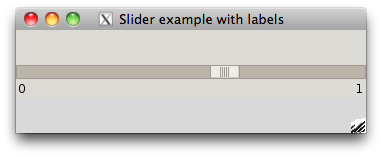
\includegraphics[width=.5\textwidth]{fig-tcltk-slider-labels.png}
  \caption{The \code{ttk::scale} widget with labels added}
  \label{fig:tcltk-slider-labels}
\end{figure}

The \constructor{ttkscale} constructor to produce a themeable scale
(slider) control is missing\footnote{As of the version of \pkg{tcltk}
  accompanying \R{} 2.13.1}. You can define your own simply enough:
\begin{Schunk}
\begin{Sinput}
 ttkscale <- function(parent, ...) 
   tkwidget(parent, "ttk::scale", ...)
\end{Sinput}
\end{Schunk}

The orientation is set through the option \option{orient}{ttkscale}
taking values of \qcode{horizontal} (the default) or
\qcode{vertical}. For sizing the slider, the \option{length}{ttkscale}
option is available.  

To set the range, the basic options are \option{from}{ttkscale} and
\option{to}{ttkscale}. There is no \code{by} option as of \TK\/
8.5. The constructor \constructor{tkscale}, for a non-themeable slider,
has the option \option{resolution}{tkscale} to set that. Additionally,
the themeable slider does not have any label or tooltip indicating its
current value.


As a workaround, we show how to display a vector of values by sliding
through the indices and place labels at the ends of the slider to
indicate the range (Figure~\ref{fig:tcltk-slider-labels}). We write
this using an \R{} reference class.

\begin{Schunk}
\begin{Sinput}
 Slider <-
   setRefClass("TtkSlider",
      fields=c("frame", "widget", "v", "x", "FUN"),
      methods=list(
        initialize=function(parent, x) {
          x <<- x;  v <<- tclVar(1)
          FUN <<- NULL                   # NULL of fuction
          frame <<- ttkframe(parent)
          widget <<- ttkscale(frame, from=1, to=length(x),
                              variable=v, orient="horizontal")
          ## For this widget, the callback is passed a value 
          ## which we ignore here
          tkconfigure(widget, command=function(...) {
            if(is.function(FUN)) FUN(.self)
          })
          layout_gui()
          .self
        },
        layout_gui=function() {         
          tkgrid(widget, row=0, column=0, columnspan=3, 
                 sticky="we")
          tkgrid(ttklabel(frame, text=x[1]), 
                 row=1, column=0)
          tkgrid(ttklabel(frame, text=x[length(x)]), 
                 row=1, column=2)
          tkgrid.columnconfigure(frame, 1, weight=1)
        },
        add_callback=function(FUN) FUN <<- FUN,
        get_value=function() x[as.numeric(tclvalue(v))],
        set_value=function(value) {
          "Set value. Value must be in x"
          ind <- match(value, x)
          if(!is.na(ind)) {
            v_local <- v
            tclvalue(v_local) <- ind
          }
        }
        ))
\end{Sinput}
\end{Schunk}

To use this, we have:
\begin{Schunk}
\begin{Sinput}
 w <- tktoplevel()
 f <- ttkframe(w, padding=c(3,3,12,12))
 tkpack(f, expand=TRUE, fill="both")
 x <- seq(0,1,by=0.05)
 ##
 s <- Slider$new(parent=w, x=x)
 tkpack(s$frame, expand=TRUE, fill="x", anchor="n")
 ##
 s$set_value(0.5)
 print(s$get_value())
\end{Sinput}
\begin{Soutput}
[1] 0.5
\end{Soutput}
\end{Schunk}

As seen in the \meth{initialize} and \meth{get\_value} methods, the
\option{variable}{ttkscale} option can be used for specifying a \TCL\/
variable to record the value of the slider. This is convenient when
the variable and widget are encapsulated into a class, as
above. Otherwise the \option{value}{ttkscale} option is available.
The \function{tkget} and \function{tkset} function (using the
\subcommand{get}{ttkscale} and \subcommand{set}{ttkscale} sub
commands) can be used to get and set the value shown. They are used in
the same manner as the same-named subcommands for a combo box.

The \meth{add\_callback} method can be used to add a callback function
when the slider changes value. We set up the call to pass back in a
reference to the object, so there is no issue with finding the \TCL\/
variable to get the value.
\begin{Schunk}
\begin{Sinput}
 s$add_callback(function(obj) print(obj$get_value()))
\end{Sinput}
\end{Schunk}


\subsection{Spin boxes}
\label{sec:tcltk:spinboxes}

A themeable spinbox is introduced in \TK\/ version 8.5.9. However,  as of
writing, the Window libraries accompanying \R{} are 8.5.8, so we will
assume there is no themeable spinbox widget. In \TK\/ the
\code{spinbox} command produces a non-themeable spinbox. Again, there
is no direct \constructor{tkspinbox} constructor, but one can be
defined with:\footnote{One could compare the result of
  \code{tcl("info", "patchlevel")} to 8.5.9 and use
  \qcode{ttk::spinbox} if the libraries support it.}
\begin{Schunk}
\begin{Sinput}
 tkspinbox <- function(parent, ...) 
     tkwidget(parent, "tk::spinbox", ...)
\end{Sinput}
\end{Schunk}

The non-themeable widgets have many more options than the themeable
ones, as style properties can be set on a per-widget basis. We won't
discuss those here. The spinbox can be used to select from a sequence
of numeric values or a vector of character values.


For example, the following allows a user to scroll either direction through the 50
states of the U.S.

\begin{Schunk}
\begin{Sinput}
 w <- tktoplevel()
 sp <- tkspinbox(w, values=state.name, wrap=TRUE)
\end{Sinput}
\end{Schunk}

Whereas, this invocation will allow scrolling through a numeric sequence:
\begin{Schunk}
\begin{Sinput}
 sp1 <- tkspinbox(w, from=1, to=10, increment=1)
\end{Sinput}
\end{Schunk}



The basic options to set the range for a numeric spinbox are
\option{from}{tkspinbox}, \option{to}{tkspinbox}, and
\option{increment}{tkspinbox}.  The \option{textvariable}{tkspinbox}
option can be used to link the spinbox to a \TCL\/ variable. As usual,
this allows the user to easily get and set the value
displayed. Otherwise, the \function{tkget} and \function{tkset}
functions may be used for these tasks. 

As seen, in \TK, spin boxes can also be used to select from a list of
text values. These are specified through the
\option{values}{tkspinbox} option. In the \code{state.name} example
above, we set the \option{wrap}{tkspinbox} option to \code{TRUE} so
that the values wrap around when the end is reached.
 
The option \option{state}{tkspinbox} can be used to specify whether
the user can enter values, the default of \qcode{normal}; not edit the
value, but simply select one of the given values (\qcode{readonly}),
or not select a value (\qcode{disabled}).  As with a combo box, when
the \TK\/ spinbox displays character data and is in the \qcode{normal}
state, the widget can be controlled like the entry widget of
Section~\ref{sec:tcltk:entry-widgets}.



% \begin{example}{A GUI for selecting a numeric range}{ex-tcltk-doublescale}
%   \SweaveInput{ex-tcltk-doublescale}
% \end{example}

%% Too much? It ain't pretty
\begin{example}{A GUI for \code{t.test}}{ex-tcltk-t-test}
This example illustrates how the basic widgets can be combined to make
a dialog for gathering information to run a $t$-test. A realization is
shown in Figure~\ref{fig:fig-tcltk-t-test}.

%% Moved earlier in text
% \begin{figure}
%   \centering
%   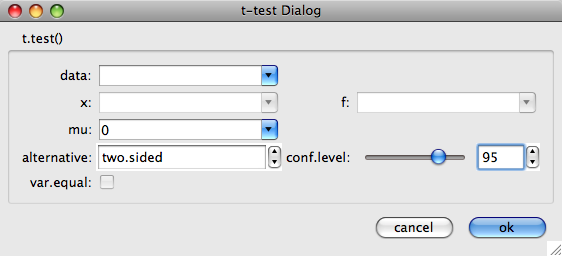
\includegraphics[width=.75\textwidth]{fig-tcltk-t-test.png}
%   \caption{A dialog to collect values for a $t$ test. This shows
%     several of the selection widgets discussed in the chapter: a check
%     button, radio button, combo boxes, an entry widget, a scale widget
%     and a spinbox.}
%   \label{fig:fig-tcltk-t-test}
% \end{figure}





We will use a data store to hold the values to be passed to
\code{t.test}. For the data store, we  use an environment to hold \Tcl\/ variables.

\begin{Schunk}
\begin{Sinput}
 e <- new.env()
 e$x <- tclVar(""); e$f <- tclVar(""); e$data <- tclVar("")
 e$mu <- tclVar(0); e$alternative <- tclVar("two.sided")
 e$conf.level <- tclVar(95); e$var.equal <- tclVar(FALSE)
\end{Sinput}
\end{Schunk}

This allows us to write a function to evaluate a $t$-test easily
enough, although we don't illustrate that.






Our layout is basic. Here we pack a label frame into the window to give the dialog a nicer look.
We will use the \code{tkgrid} geometry manager below.
\begin{Schunk}
\begin{Sinput}
 lf <- ttklabelframe(f, text="t.test()", padding=10)
 tkpack(lf, expand=TRUE, fill="both", padx=5, pady=5)
\end{Sinput}
\end{Schunk}

The grid will have four columns, with columns 0 and 2 being for labels.
We don't want the labels to expand the same way we want the widget columns to do, so we
assign different weights:
\begin{Schunk}
\begin{Sinput}
 tkgrid.columnconfigure(lf, 0, weight=1)
 tkgrid.columnconfigure(lf, 1, weight=10)
 tkgrid.columnconfigure(lf, 2, weight=1)
 tkgrid.columnconfigure(lf, 1, weight=10)
\end{Sinput}
\end{Schunk}


This helper function simplifies the task of adding a label.
\begin{Schunk}
\begin{Sinput}
 putLabel <- function(parent, text, row, column) {
   label <- ttklabel(parent, text=text)
   tkgrid(label, row=row, column=column, sticky="e")
 }
\end{Sinput}
\end{Schunk}
%

Our first widget will be one to select a data frame. For this, a
combo box is used, although if a large number of data frames are a
possibility, a different widget may be better suited. Also not shown are two
similar calls to create combo boxes \code{xCombo} and \code{fCombo}
which allow the user to specify parts of a formula.

\begin{Schunk}
\begin{Sinput}
 putLabel(lf, "data:",0,0)
 dataCombo <- ttkcombobox(lf, state="readonly", 
                          values=ProgGUIinR:::avail_dfs(), 
                          textvariable=e$data)
 tkgrid(dataCombo, row=0, column=1, sticky="ew", padx=2)
 tkfocus(dataCombo)                      # give focus
\end{Sinput}
\end{Schunk}



We use a \constructor{ttkentry} widget for the user to specify
a mean. For this purpose, the use is straightforward.
\begin{Schunk}
\begin{Sinput}
 putLabel(lf, "mu:", 2, 0)
 muCombo <-  ttkentry(lf,  textvariable=e$mu)
 tkgrid(muCombo, row=2, column=1, sticky="ew", padx=2)
\end{Sinput}
\end{Schunk}

The selection of an alternative hypothesis is a natural choice for a
combo box or a radio button group, we use the latter.
\begin{Schunk}
\begin{Sinput}
 putLabel(lf, "alternative:", 3, 0)
 rbFrame <- ttkframe(lf)
 sapply(c("two.sided","less","greater"), function(i) {
   rb <- ttkradiobutton(rbFrame, variable=e$alternative, 
                        text=i, value=i)
   tkpack(rb, side="left")
 })
 tkgrid(rbFrame, row=3, column=1, sticky="ew", padx=2)
\end{Sinput}
\end{Schunk}

Here we use a range widget to specify the confidence level. The slider
is quicker to use, but less precise than the spinbox. By sharing a
text variable, the widgets are automatically synchronized.
\begin{Schunk}
\begin{Sinput}
 putLabel(lf, "conf.level:", 3, 2)
 confFrame <- ttkframe(lf)
 tkgrid(confFrame, row=3, column=3, columnspan=2, 
        sticky="ew", padx=2)
 ##
 confScale <- ttkscale(confFrame, from=75, to=100, 
                      variable=e$conf.level)
 confSpin <- tkspinbox(confFrame, from=75, to=100, increment=1, 
                      textvariable=e$conf.level, width=5)
 ##
 tkpack(confScale, expand=TRUE, fill="y", side="left")
 tkpack(confSpin, side="left")
\end{Sinput}
\end{Schunk}

A checkbox is used to collect the logical value for \code{var.equal}:
\begin{Schunk}
\begin{Sinput}
 putLabel(lf, "var.equal:", 4, 0)
 veCheck <- ttkcheckbutton(lf, variable=e$var.equal)
 tkgrid(veCheck, row=4, column=1, stick="w", padx=2)
\end{Sinput}
\end{Schunk}


The dialog has standard "cancel" and "ok" buttons.
\begin{Schunk}
\begin{Sinput}
 bf <- ttkframe(f)
 cancel <- ttkbutton(bf, text="cancel")
 ok <- ttkbutton(bf, text="ok")
 #
 tkpack(bf, fill="x", padx=5, pady=5)
 tkpack(ttklabel(bf, text=" "), expand=TRUE, fill="y", 
        side="left")                     # add a spring
 sapply(list(cancel, ok), tkpack, side="left", padx=6)
\end{Sinput}
\end{Schunk}
%

For the \code{ok} button we want to gather the values and run the
function. The \code{runTTest} function does this.  We configure both
buttons, then add to the default button bindings to invoke either of the button's commands
when they have the focus and \kbd{return} is pressed.
\begin{Schunk}
\begin{Sinput}
 tkconfigure(ok, command=runTTest)
 tkconfigure(cancel, command=function() tkdestroy(w))
 tkbind("TButton", "<Return>", function(W) tcl(W, "invoke"))
\end{Sinput}
\end{Schunk}

At this point, our GUI is complete, but we would like to have it
reflect any changes to the underlying \R\/ environment that effect its
display. A such, we define
a function, \code{updateUI}, which does two basic things: it searches for
new data frames and it adjusts the controls depending on the current
state.
\begin{Schunk}
\begin{Sinput}
 updateUI <- function() {
   dfName <- tclvalue(e$data)
   curDfs <- ProgGUIinR:::avail_dfs()
   tkconfigure(dataCombo, values=curDfs)
   if(!dfName %in% curDfs) {
     dfName <- ""
     tclvalue(e$data) <- ""
   }
 
   if(dfName == "") {
     ## 3 ways to disable needed!!
     x <- list(xCombo, fCombo, muCombo,  confScale, veCheck, ok)
     sapply(x, function(W) tcl(W, "state", "disabled"))
     sapply(as.character(tkwinfo("children", rbFrame)), 
            function(W) tcl(W, "state", "disabled"))
     tkconfigure(confSpin, state="disabled")
   } else {
     ## enable univariate, ok
     sapply(list(xCombo,  muCombo, confScale, ok),
            function(W) tcl(W, "state", "!disabled"))
     sapply(as.character(tkwinfo("children", rbFrame)), 
            function(W) tcl(W, "state", "!disabled"))
     tkconfigure(confSpin, state="normal")
     
     df <- get(dfName, envir=.GlobalEnv)
     numVars <- getNumericVars(df)
     tkconfigure(xCombo, values=numVars)
     if(! tclvalue(e$x) %in% numVars)
       tclvalue(e$x) <- ""
 
     ## bivariate
     availFactors <- getTwoLevelFactor(df)
     sapply(list(fCombo, veCheck),
            function(W) {
              val <- if(length(availFactors)) "!" else ""
              tcl(W, "state", sprintf("%sdisabled", val))
            })
     tkconfigure(fCombo, values=availFactors)
     if(!tclvalue(e$f) %in% availFactors)
       tclvalue(e$f) <- ""
       
          }
 }
 updateUI()
 tkbind(dataCombo, "<<ComboboxSelected>>", updateUI)
\end{Sinput}
\end{Schunk}

This function could be bound to a ``refresh'' button or we could
arrange to have it called in the background. Using the \code{after}
command we could periodically check for new data frames, using a
\iprogram{task callback}task callback we can call this every time a
new command is issued.  As the call could potentially be costly, we
only call if the available data frames have been changed. Here is one
way to arrange that:
\begin{Schunk}
\begin{Sinput}
 require(digest)
 create_function <- function() {
   .dfs <- digest(ProgGUIinR:::avail_dfs())
   f <- function(...) {
     if((val <- digest(ProgGUIinR:::avail_dfs())) != .dfs) {
       .dfs <<- val
       updateUI()
     }
     return(TRUE)
   }
 }
\end{Sinput}
\end{Schunk}
Then to create a task callback we have
\begin{Schunk}
\begin{Sinput}
 id <- addTaskCallback(create_function())
\end{Sinput}
\end{Schunk}

% <<>>=
% updateUI()                              # run once
% tkbind("TCombobox","<<ComboboxSelected>>", updateUI) ## misses update on new data
% @ 
\end{example}


\chapter{Tcl/Tk: Text, Tree and Canvas Widgets}
\label{sec:tcltk:scrollable-widgets}
This chapter focuses on a few of the more complex widgets of \Tk,
primarily the text widget, the treeview widget and the canvas
widget.

\section{Scrollbars}
\label{sec:tcltk:scrollbars}

\TK\/ has several scrollable widgets -- those that use scrollbars.
Widgets which accept a scrollbar (without too many extra steps) have
the options \code{xscrollcommand} and \code{yscrollcommand}.  For
these, to use scrollbars in \pkg{tcltk} requires two steps: the
scrollbars must be constructed and bound to some widget, and that
widget must be told it has a scrollbar. This way changes to the widget
can update the scrollbar and vice versa. Suppose, \code{parent} is a
container and \code{widget} has these options, then the following will
set up both horizontal and vertical scrollbars.
%
\begin{Schunk}
\begin{Sinput}
 xscr <- ttkscrollbar(parent, orient="horizontal",
                  command=function(...) tkxview(widget, ...))
 yscr <- ttkscrollbar(parent, orient="vertical",
                  command=function(...) tkyview(widget, ...))
\end{Sinput}
\end{Schunk}
%
The \function{tkxview} and \function{tkyview} functions set what part of the widget is being shown.

To link the widget back to the scrollbar, the \code{set} command is
used in a callback to the scroll command.  For this example we
configure the options after the widget is constructed, but this can be
done at the time of construction as well. Again, the command takes a
standard form:
\begin{Schunk}
\begin{Sinput}
 tkconfigure(widget,
             xscrollcommand=function(...) tkset(xscr,...),
             yscrollcommand=function(...) tkset(yscr,...))
\end{Sinput}
\end{Schunk}

Although scrollbars can appear anywhere, the conventional place is on
the right and lower side of the parent. The following adds scrollbars
using the grid manager. The combination of weights and stickiness below
will have the scrollbars expand as expected if the window is resized.
\begin{Schunk}
\begin{Sinput}
 tkgrid(widget, row=0, column=0, sticky="news")
 tkgrid(yscr,row=0,column=1, sticky="ns")
 tkgrid(xscr, row=1, column=0, sticky="ew")
 tkgrid.columnconfigure(parent, 0, weight=1)
 tkgrid.rowconfigure(parent, 0, weight=1)
\end{Sinput}
\end{Schunk}
%
Although this is a bit tedious, it does give the programmer some
flexibility in arranging scrollbars. For subsequent usage, we turn the above into the
function \function{addScrollbars} (not shown). In
base \Tk, there are no simple means to hide scrollbars when not
needed, although the \pkg{tcltk2} package has some code that may be
employed for that.


\section{Multi-line text widgets}
\label{sec:tcltk:multi-line-text}

The \constructor{tktext} widget creates a multi-line text editing
widget. If constructed with no options but a parent container, the
widget can have text entered into it by the user:

\begin{Schunk}
\begin{Sinput}
 w <- tktoplevel()
 tkwm.title(w, "Simple tktext example")
 txt <- tktext(w)
 addScrollbars(w, txt)
\end{Sinput}
\end{Schunk}
%

%% arguments width, height
The text widget is not a themed widget, hence has numerous arguments
to adjust its appearance. We mention a few here and leave the rest to
be discovered in the manual page (along with much else). The argument
\argument{width}{tktext} and \argument{height}{tktext} are there to
set the initial size, with values specifying number of characters and
number of lines (not pixels, to convert see
Section~\ref{sec:tcltk:overview:colors-fonts}). The actual size is
font dependent, with the default for 80 by 24 characters. The
\argument{wrap}{tktext} argument, with a value from \qcode{none},
\qcode{char}, or \qcode{word}, indicates if wrapping is to occur and
if so, does it happen at any character or only a word boundary. The
argument \argument{undo}{tktext} takes a logical value indicating if
the undo mechanism should be used. If so, the subcommand
\subcommand{edit}{tktext} can be used to undo a change (or the
\kbd{control-z} keyboard shortcut).

\paragraph{Inserting text}
Inserting text can be done through the \subcommand{insert}{ttktext}
subcommand. This shows how one can use \code{$\backslash$n} to add new
lines:
\begin{Schunk}
\begin{Sinput}
 tkinsert(txt, 
          "1.0", 
          paste("Lorem ipsum dolor",
                "sit amet,", sep="\n"))
\end{Sinput}
\end{Schunk}
Images and other windows can be added to a text buffer, but we do not
discuss that here. The value \qcode{1.0} is an index (described below)
marking the beginning of the buffer.

\paragraph{Getting text}
%% multiline? tclvalue versus as.character
The \subcommand{get}{tktext} subcommand is used to retrieve the text
in the buffer. One specifies what part of the text buffer should be
returned using indices. The following shows how to retrieve the entire
contents of the buffer:

\begin{Schunk}
\begin{Sinput}
 value <- tkget(txt, "1.0", "end")
 as.character(value)                     # wrong way
\end{Sinput}
\begin{Soutput}
[1] "Lorem" "ipsum" "dolor" "sit"   "amet,"
\end{Soutput}
\begin{Sinput}
 tclvalue(value)
\end{Sinput}
\begin{Soutput}
[1] "Lorem ipsum dolor\nsit amet,\n"
\end{Soutput}
\end{Schunk}

The return value is of class \class{tclObj}.  The above example shows
that coercion to character
should be done with \function{tclvalue} and not
\function{as.character} to preserve the distinction between spaces and
line breaks.


\paragraph{Indices}
As with the entry widget, several commands take indices to specify
position within the text buffer. Only for the multi-line widget both a
line and character are needed in some instances. These indices may be
specified in many ways. One can use row and character numbers
separated by a period in the pattern \code{line.char}. The line is
$1$-based, the column $0$-based (e.g., \code{1.0} says start on the
1st row and first character). In general, one can specify any line number and character on
that line, with the keyword \code{end} used to refer to the last
character on the line.

Text buffers may carry transient marks, in which case the use of this
mark indicates the next character after the mark. Predefined marks
include \code{end}, to specify the end of the buffer, \code{insert},
to track the insertion point in the text buffer were the user to begin
typing, and \code{current}, which follows the character closest to the
mouse position.

%% use of index and mark
The specification
\begin{Schunk}
\begin{Sinput}
 value <- tkget(txt, "1.0", "end")
\end{Sinput}
\end{Schunk}
uses the index \code{1.0} to refer to the beginning of the buffer and
the mark \qcode{end} to refer to the character after the end.

%% tags
As well, pieces of text may be tagged. The format \code{tag.first} and
\code{tag.last} index the range of the tag \code{tag}. Marks and tags
are described further below. If the $x$-$y$ postion of the spot is known
(through percent substitutions say) the index can be specified by
postion, as \code{\@x,y}.

Indices can also be adjusted relative to the above
specifications. This adjustment can be by a number of characters
(\code{chars}), index positions (\code{indices}) or \code{lines}. For
example, \code{insert + 1 lines} refers to 1 line under the insert
point. The values \code{linestart}, \code{lineend}, \code{wordstart}
and \code{wordend} are also available. For instance, \code{insert
  linestart} is the beginning of the line from the insert point, while
\code{end -1 wordstart} and \code{end - 1 chars wordend} refer to the
beginning and ending of the last word in the buffer. (The \code{end}
index refers to the character just after the new line so we go back 2
steps.)

\paragraph{Deleting text}

The text between two indices can be deleted using \code{tkdelete}, as
with \code{tkdelete(txt, "1.0", "end")}, which would clear the entire
buffer's contents.

\paragraph{Panning the buffer: \code{tksee}}
After text is inserted, the visible part of buffer may not be what is
desired. The \subcommand{see}{ttktext} sub command is used to position
the buffer on the specified index, its lone argument.


\paragraph{Tags}
Tags are a means to assign a name to characters within the text
buffer. Tags may be used to adjust the foreground, background and font
properties of the tagged characters from those specified globally at
the time of construction of the widget, or configured thereafter. Tags
can be set when the text is inserted by appending to the argument
list, as with
\begin{Schunk}
\begin{Sinput}
 tkinsert(txt, "end", "last words", "lastWords") # lastWords tag
\end{Sinput}
\end{Schunk}

Tags can be set after the text is added through the
\subcommand{tag add}{tktext} subcommand using indices to specify
location. The following marks the first word with the \code{firstWord}
tag:
\begin{Schunk}
\begin{Sinput}
 tktag.add(txt, "firstWord", "1.0 wordstart", "1.0 wordend")
\end{Sinput}
\end{Schunk}
The \subcommand{tag configure}{tktext} can be used to configure properties of the tagged characters, for example:
\begin{Schunk}
\begin{Sinput}
 tktag.configure(txt, "firstWord", foreground="red", 
                 font="helvetica 12 bold")
\end{Sinput}
\end{Schunk}
%
There are several other configuration options for a tag. From within
an \R\/ session, a cryptic list can be produced by calling the
subcommand \subcommand{tag configure}{tktext} without a value for
configuration.


\paragraph{Selection}
The current selection, if any, is indicated by the \code{sel} tag,
with \code{sel.first} and \code{sel.last} providing indices to refer
to the selection (assuming the option \code{exportSelection} was not
modified). These tags can be used with \code{tkget} to retrieve the
currently selected text. An error will be thrown if there is no
current selection. To check if there is a current selection, the following may be used:
\begin{Schunk}
\begin{Sinput}
 hasSelection <- function(W) {
   ranges <- tclvalue(tcl(W, "tag", "ranges", "sel"))
   length(ranges) > 1 || ranges != ""
 }
\end{Sinput}
\end{Schunk}

\paragraph{Cut, copy and paste} \iprogram{clipboard}
The cut, copy and paste commands are implemented through the \Tk\/ functions
\function{tk\_textCut}, \function{tk\_textCopy} and
\function{tk\_textPaste}. Their lone argument is the text widget. These
work with the current selection and insert point. For example to cut
the current selection, one has
\begin{Schunk}
\begin{Sinput}
 tcl("tk_textCut", txt)
\end{Sinput}
\end{Schunk}

\paragraph{Marks}
Tags mark characters within a buffer, marks denote positions within a
buffer that can be modified. For example, the marks \code{insert} and
\code{current} refer to the position of the cursor and the current
position of the mouse. Such information can be used to provide
context-sensitive popup menus, as in this code example:
\begin{Schunk}
\begin{Sinput}
 popupContext <- function(W, x, y) {
   ## or use sprintf("@%s,%s", x, y) for "current"
   cur <- tkget(W, "current wordstart", "current wordend") 
   cur <- tclvalue(cur)
   popupContextMenuFor(cur, x, y)        # some function
 }
\end{Sinput}
\end{Schunk}

To assign a new mark, one uses the \subcommand{mark set}{tktext}
subcommand specifying a name and a position through an index. Marks
refer to spaces within characters. The \code{gravity} of the mark can
be \code{left} or \code{right}. When \code{right} (the default), new
text inserted is to the left of the mark. For instance, to keep track
of an initial insert point and the current one, the initial point
(marked \code{leftlimit} below) can be marked with
\begin{Schunk}
\begin{Sinput}
 tkmark.set(txt, "leftlimit", "insert")
 tkmark.gravity(txt, "leftlimit", "left")    # keep on left
 tkinsert(txt, "insert", "new text")
 tkget(txt, "leftlimit", "insert")
\end{Sinput}
\begin{Soutput}
<Tcl> new text 
\end{Soutput}
\end{Schunk}
%
The use of the subcommand \subcommand{mark gravity}{tktext} is done so
that the mark attaches to the left-most character at the insert
point. The rightmost one changes as more text is inserted, so would
make a poor choice here.


\paragraph{The edit command}
The subcommand \subcommand{edit}{tktext} can be used to undo text. As
well, it can be used to test if the buffer has been modified, as
follows:
\begin{Schunk}
\begin{Sinput}
 tcl(txt, "edit", "undo")                  # no output
 tcl(txt, "edit", "modified")              # 1 = TRUE
\end{Sinput}
\begin{Soutput}
<Tcl> 1 
\end{Soutput}
\end{Schunk}



\paragraph{Events}
The text widget has a few important events.  The widget defines
virtual events \code{\VirtualEvent{Modified}} and
\code{\VirtualEvent{Selection}} indicating when the buffer is modified
or the selection is changed. Like the single-line text widget, the
events \code{\Event{KeyPress}} and \code{\Event{KeyRelease}} indicate
key activity. The \%-substitution \code{k} gives the keycode and
\code{K} the key symbol as a string (\code{N} is the decimal number).



\begin{example}{Displaying commands in a text buffer}{ex-tcltk-text}
This example shows how a text buffer can be used to display the output
of \R\/ commands, using an approach modified from \pkg{Sweave}.  We
envision this as a piece of a larger GUI which generates the commands
to evaluate. For this example though, we make a simple GUI
(Figure~\ref{fig:tcltk-text-buffer-commands}).

\begin{figure}
  \centering
  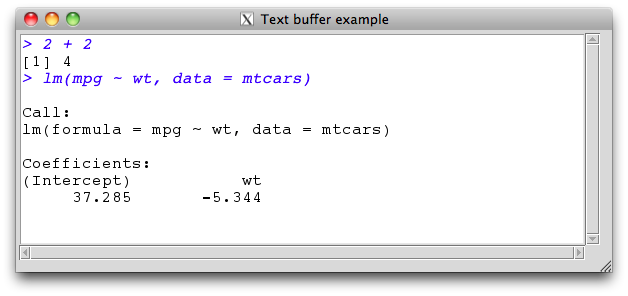
\includegraphics[width=.8\textwidth]{fig-tcltk-text-buffer-commands.png}
  \caption{A text widget used to show formatted \R{} commands and their output}
  \label{fig:tcltk-text-buffer-commands}
\end{figure}

\begin{Schunk}
\begin{Sinput}
 w <- tktoplevel(); tkwm.title(w, "Text buffer example")
 f <- ttkframe(w, padding=c(3,3,12,12))
 tkpack(f, expand=TRUE, fill="both")
 txt <- tktext(f, width=80, height = 24)   # default size
 addScrollbars(f, txt)
\end{Sinput}
\end{Schunk}
 
To distinguish between commands and their output we define the
following tags:
\begin{Schunk}
\begin{Sinput}
 tktag.configure(txt, "commandTag", foreground="blue", 
                 font="courier 12 italic")
 tktag.configure(txt, "outputTag", font="courier 12")
 tktag.configure(txt, "errorTag", foreground="red", 
                 font="courier 12 bold")
\end{Sinput}
\end{Schunk}

The following function does the work of evaluating a command chunk
then inserting the values into the text buffer, using the different
markup tags specified above to indicate commands from output.

\begin{Schunk}
\begin{Sinput}
 evalCmdChunk <- function(txt, cmds) {
   
   cmdChunks <- try(parse(text=cmds), silent=TRUE)
   if(inherits(cmdChunks,"try-error")) {
     tkinsert(t, "end", "Error", "errorTag") # add markup tag
   }
 
   for(cmd in cmdChunks) {
     cutoff <- 0.75 * getOption("width")
     dcmd <- deparse(cmd, width.cutoff = cutoff)
     command <- 
       paste(getOption("prompt"),
             paste(dcmd, collapse=paste("\n", 
                           getOption("continue"), sep="")),
             sep="", collapse="")
     tkinsert(txt, "end", command, "commandTag")
     tkinsert(txt, "end","\n")
     ## output, should check for errors in eval!
     output <- capture.output(eval(cmd, envir=.GlobalEnv))
     output <- paste(output, collapse="\n")
     tkinsert(txt, "end", output, "outputTag")
     tkinsert(txt, "end","\n")
   }
 }
\end{Sinput}
\end{Schunk}



This is how it can be used.
\begin{Schunk}
\begin{Sinput}
 evalCmdChunk(txt, "2 + 2; lm(mpg ~ wt, data=mtcars)")
\end{Sinput}
\end{Schunk}
\end{example}



\section{Menus}
\label{sec:tcltk:menus}

Menubars and popup menus in \Tk\/ are constructed with
\constructor{tkmenu}. The \code{parent} argument depends on what the menu is
to do. A toplevel menubar, such as appears at the top of a window has
a toplevel window as its parent; a submenu of a menubar uses the
parent menu; and a popup menu uses a widget.  

The menu widget in \Tk\/ has an option to be ``torn off.'' This
feature was at one time common in GUIs, but now is rarely seen so it
is recommended that this option be disabled. The
\argument{tearoff}{tkmenu} option can be used at construction time to
override the default behavior. Otherwise, the following command will
do so globally:
\begin{Schunk}
\begin{Sinput}
 tcl("option","add","*tearOff", 0)    # disable tearoff menus
\end{Sinput}
\end{Schunk}
%

A toplevel menubar is attached to a top-level window using \code{tkconfigure}
to set the \code{menu} option of the window. For the aqua \TK\/
libraries for Mac OS X, this menu will appear on the top menubar when
the window has the focus. For other operating systems, it appears at
the top of the window. For Mac OS X, a default menubar with no
relationship to your application will be shown if a menu is not
provided for a toplevel window. Testing for native Mac OS X may be done via
the following function:
\begin{Schunk}
\begin{Sinput}
 usingMac <- function()  
   as.character(tcl("tk", "windowingsystem")) == "aqua"
\end{Sinput}
\end{Schunk}

The \function{tkpopup} function facilitates the creation of a popup
menu.  This function has arguments for the menubar, and the postion
where the menu should be popped up. For example, the following code
will bind a popup menu, \code{pmb} (yet to be defined), to the right click event for a
button \code{b}. As \OSX\/ may not have a third mouse button, and when
it does it refers to it differently, the callback is bound
conditionally to different events.


\begin{Schunk}
\begin{Sinput}
 doPopup <- function(X, Y) tkpopup(pmb, X, Y) # define callback
 if (usingMac()) {
   tkbind(b, "<Button-2>", doPopup)      # right click
   tkbind(b, "<Control-1>", doPopup)     # Control + click
 } else {
   tkbind(b, "<Button-3>", doPopup)
 }
\end{Sinput}
\end{Schunk}


\paragraph{Adding submenus and action items}
Menus show a hierarchical view of action items. Items are added to a
menu through the \subcommand{add}{tkmenu} subcommand.  The nested
structure of menus is achieved by specifying a \code{tkmenu} object as
an item, using the \subcommand{add cascade}{tkmenu} subcommand. The
option \code{label} is used to label the menu and the \code{menu}
option to specify the sub-menu.

Grouping of similar items can be done through nesting, or, on occasion,
through visual separation. The latter is implemented with the \subcommand{add
  separator}{tkmenu} subcommand.


There are a few different types of action items that can be added:
 
\begin{description}
\item[Commands] An action item is one associated with a command. The
  simplest proxy is a button in the menu that activates a command when
  selected with the mouse. The \subcommand{add command}{tkmenu} allows
  one to specify a \code{label}, a \code{command} and optionally an
  \code{image} with a value for \code{compound} to adjust its
  layout. Action commands may %% (Images are not shown in Mac OS X.) 
  possibly be called for different widgets, so the use of percent
  substitution is problematic. One can also specify that a keyboard
  shortcut be displayed through the option \code{accelerator}, but
  a separate callback must listen for this combination.

\item[Check boxes] Action items may also be proxied by checkboxes. To
  create one, the subcommand \subcommand{add checkbutton}{tkmenu} is
  used. The available arguments include \code{label} to specify the
  text, \code{variable} to specify a \TCL{} variable to store the state,
  \code{onvalue} and \code{offvalue} to specify the state to the tcl
  variable, and \code{command} to specify a call back when the checked
  state is toggled. The initial state is set by the value in the
  \TCL\/ variable.

\item[Radio buttons] Additionally, action items may be presented
  through radiobutton groups. These are specified with the subcommand
  \subcommand{add radiobutton}{tkmenu}. The \code{label} option is
  used to identify the entry, \code{variable} to set a text variable
  and to group the buttons that are added, and \code{command} to
  specify a command when that entry is selected.
\end{description}

Action items can also be placed after an item, rather than at the end
using the \subcommand{insert command index}{tkmenu} subcommand. The
index may be specified numerically with 0 being the first item for a
menu.  More conveniently the index can be determined by specifying a
pattern to match against the menu's current labels.


\paragraph{Set state}
The \code{state} option is used to retrieve and set the current state
of the a menu item.  This value is typically \code{normal} or
\code{disabled}, the latter to indicate the item is not available. The
state can be set when the item is added or configured after that fact,
through the \subcommand{entryconfigure}{tkmenu} command. This function
needs the menubar specified and the item specified as an index or
pattern to match the labels.

\begin{example}{Simple menu example}{ex-tcltk-menu}
%%
This example shows how one might make a very simple code editor using
a text-entry widget. \iprogram{evaluate strings}We use the \pkg{svMisc} package, as it defines a
few GUI helpers which we use.
\begin{Schunk}
\begin{Sinput}
 library(svMisc)                         # for some helpers
 showCmd <- function(cmd) {
   writeLines(captureAll(parseText(cmd)))
 }
\end{Sinput}
\end{Schunk}

We begin with a simple GUI comprised of a top-level window containing
the text entry widget.
\begin{Schunk}
\begin{Sinput}
 w <- tktoplevel()
 tkwm.title(w, "Simple code editor")
 f <- ttkframe(w, padding=c(3,3,12,12)) 
 tkpack(f, expand=TRUE, fill="both")
 tb <- tktext(f, undo=TRUE)
 addScrollbars(f, tb)
\end{Sinput}
\end{Schunk}
%

Using \function{tkmenu}, we create a toplevel menubar, \code{mb}, and
attach it to our toplevel window. Following that, we make ``file'' and ``edit'' submenus.
\begin{Schunk}
\begin{Sinput}
 mb <- tkmenu(w); tkconfigure(w, menu=mb)
 fileMenu <- tkmenu(mb)
 tkadd(mb, "cascade", label="File", menu=fileMenu)
 #
 editMenu <- tkmenu(mb)
 tkadd(mb, "cascade", label="Edit", menu=editMenu)
\end{Sinput}
\end{Schunk}
%

To these sub menubars, we add action items. First a command to
evaluate the contents of the buffer.
\begin{Schunk}
\begin{Sinput}
 tkadd(fileMenu, "command", label="Evaluate buffer",
       command = function() {
         curVal <- tclvalue(tkget(tb, "1.0", "end"))
         showCmd(curVal)
       })
\end{Sinput}
\end{Schunk}

Then a command to evaluate just the current selection
\begin{Schunk}
\begin{Sinput}
 tkadd(fileMenu, "command", label="Evaluate selection",
       state="disabled",
       command = function() {
         curSel <- tclvalue(tkget(tb, "sel.first", "sel.last"))
         showCmd(curSel)
       })
\end{Sinput}
\end{Schunk}

Finally, we end the file menu with a quit action. 
\begin{Schunk}
\begin{Sinput}
 tkadd(fileMenu, "separator")
 tkadd(fileMenu, "command", label="Quit", 
       command=function() tkdestroy(w))
\end{Sinput}
\end{Schunk}

The edit menu has an undo and redo item. For illustration purposes we add an icon to the undo item.
\begin{Schunk}
\begin{Sinput}
 img <- system.file("images","up.gif", package="gWidgets")
 tkimage.create("photo", "::img::undo", file=img)
 tkadd(editMenu, "command", label="Undo",
       image="::img::undo", compound="left", state="disabled",
       command = function() tcl(tb, "edit", "undo"))
 tkadd(editMenu, "command", label="Redo", state="disabled",
       command = function() tcl(tb, "edit", "redo"))
\end{Sinput}
\end{Schunk}

For updating the GUI, we want to configure the menu items to reflect
if the current buffer has a selection or can undo or redo. To check
the selection we have:
\begin{Schunk}
\begin{Sinput}
 tkbind(tb, "<<Selection>>", function(W) {
   hasSelection <- function(W) {
     ranges <- tclvalue(tcl(W, "tag", "ranges", "sel"))
     length(ranges) > 1 || ranges != ""
   }
   ## configure using an index
   sel_state <- ifelse(hasSelection(W), "normal", "disabled")
   tkentryconfigure(fileMenu, 1, state=sel_state)
 })
\end{Sinput}
\end{Schunk}
%%
To check for do and undo, we bind to the \code{Modified} virtual event.
\begin{Schunk}
\begin{Sinput}
 tkbind(tb, "<<Modified>>", function(W) {
   ## not really can_undo/can_redo but nothing suitable
   can_undo <- as.logical(tcl(W,"edit", "modified"))
   undo_state <- ifelse(can_undo, "normal", "disabled")
   sapply(c("Undo", "Redo"), function(i)        # match pattern
          tkentryconfigure(editMenu, i, state=undo_state)) 
 })
\end{Sinput}
\end{Schunk}


We add a shortcut entry to the menubar and a binding to the
top-level window for the keyboard shortcut for ``undo.''
\begin{Schunk}
\begin{Sinput}
 if(usingMac()) {
   tkentryconfigure(editMenu, "Undo", accelerator="Cmd-z")
   tkbind(w, "<Option-z>", function() tcl(tb, "edit", "undo"))
 } else {
   tkentryconfigure(editMenu, "Undo", accelerator="Control-u")
   tkbind(w, "<Control-u>", function() tcl(tb, "edit", "undo"))
 }
\end{Sinput}
\end{Schunk}
%

To illustrate popup menus, we define one within our text widget that
will grab all functions that complete the current word, using the
\function{completion} function from the \pkg{svMisc} package to
provide the completions.  The use of \code{current wordstart} and
\code{current wordend}, below, to find the word at the insertion point
isn't quite right for \R, as it stops at periods, but we don't pursue
fixing this.
\begin{Schunk}
\begin{Sinput}
 doPopup <- function(W, X, Y) {
   cur <- tclvalue(tkget(W, "current  wordstart", 
                            "current wordend"))
   tcl(W, "tag", "add", "popup", "current  wordstart", 
                                 "current wordend")
   posVals <- head(completion(cur)[,1, drop=TRUE], n=20)
   if(length(posVals) > 1) {
     popup <- tkmenu(tb)                # create menu for popup
     sapply(posVals, function(i) {         
       tkadd(popup, "command", label=i, command = function() {
         tcl(W,"replace", "popup.first", "popup.last", i)
       })
     })
     tkpopup(popup, X, Y)
  }}
\end{Sinput}
\end{Schunk}

For a popup, we set the appropriate binding for the underlying
windowing system. For the second mouse button binding in OS X, we
clear the clipboard. Otherwise the text  will be pasted in, as this mouse
action already has a default binding for the text widget.

\begin{Schunk}
\begin{Sinput}
 if (!usingMac()) {
   tkbind(tb, "<Button-3>", doPopup)
 } else {
   tkbind(tb, "<Button-2>", function(W,X,Y) {
     ## UNIX legacy re mouse-2 click for selection copy
     tcl("clipboard","clear",displayof=W) 
     doPopup(W,X,Y)
     })      # right click
   tkbind(tb, "<Control-1>", doPopup)     # Control + click
 }
\end{Sinput}
\end{Schunk}
\end{example}



\section{Treeview widget}
\label{sec:tcltk:treeview-widget}

The themed treeview widget can be used to display rectangular data,
like a data frame; or hierarchical data, like a list. The usage is
similar, but for a minor change to indicate the hierarchical structure.

\subsection{Rectangular data}

\XXX{Images -- add comment}

%% constructor
The \constructor{ttktreeview} constructor creates the tree
widget. There is no separate model for this widget, as there is in
\GTK{} or \Qt, but there is a means to adjust what is displayed.  The
argument \argument{columns}{ttktreeview} is used to specify internal
names for the columns and indicate the number of columns. A value of
\code{1:n} will work here unless explicit names are desired. The
argument \argument{displaycolumns}{ttktreeview} is used to control
which of the columns are actually displayed. The default is
\qcode{all}, but a vector of indices or names can be given.  

The size of the widget is specified two different ways.  The
\argument{height}{ttktreeview} argument is used to adjust the number
of visible rows. The requested width of the widget is determined by
the combined widths of each column, whose adjustments are mentioned
later.



If \code{f} is a frame, then the following call will create a treeview
widget with just one column showing 25 rows at a time, like the older,
non-themed, listbox widget of \Tk.

\begin{Schunk}
\begin{Sinput}
 tr <- ttktreeview(f, 
                   columns=1,        # column identifier is "1"
                   show="headings",  # not "#0"
                   height=25)        
 addScrollbars(f, tr)                # our scrollbar function
\end{Sinput}
\end{Schunk}



The treeview widget has an initial column for showing the tree-like
aspect with the data. This column is referenced by \code{\#0}. The
\argument{show}{ttktreeview} argument controls whether this column is
shown. A value of \qcode{tree} leaves just this column shown,
\qcode{headings} will show the other columns, but not the first, and
the combined value of \qcode{tree headings} will display both (the
default).  Additionally, the treeview is a scrollable widget, so has
the arguments \argument{xscrollcommand}{ttktreeview} and
\argument{yscrollcommand}{ttktreeview} for specifying scrollbars.

\paragraph{Adding values}

Rectangular data has a row and column structure. In \R, data frames
are internally stored by column vectors, so each column may have its
own type. The treeview widget is different, it stores all data as
character data and one interacts with the data row by row.

Values can be added to the widget through the
\subcommanda{insert}{ttktreeview}{parent item [text] [values]}
subcommand. This requires the specification of a parent (always the root
\qcode{} for rectangular data) and an index for specifying the
location of the new child amongst the previous children. The special
value \qcode{end} indicates placement after all other children, as
would a number larger than the number of children. A value of 0 or a
negative value would put it at the beginning.


In the example this is how we can add a list of possible CRAN mirrors
to the treeview display.
\begin{Schunk}
\begin{Sinput}
 x <- getCRANmirrors()
 Host <- x$Host
 shade <- c("none", "gray")                     # tag names
 for(i in seq_along(Host))
   ID <- tkinsert(tr, "", "end", values=as.tclObj(Host[i]),
                  tag=shade[i %% 2])            # none or gray
 tktag.configure(tr, "gray", background="gray95") # shade rows
\end{Sinput}
\end{Schunk}

For filling in each row's content the \code{values} option is used. If
there is a single column, like the current example, care needs to be
taken when adding a value. The call to \function{as.tclObj} prevents
the widget from dropping values after the first space.\footnote{As
  does wrapping the values within braces.} Otherwise, we can pass a
character vector of the proper length.


There are a number of other options for each row. If column \code{\#0}
is present, the \code{text} option is used to specify the text for the
tree row and the option \code{image} can be given to specify an image
to place to the left of the text value. Finally, we mention the
\code{tag} option for \code{insert} that can be used to specify a tag
for the inserted row. This allowed the use of the subcommand
\subcommand{tag configure}{ttktreeview} to configure the background
color. In addition, one can adjust foreground color, font or image for
an item.



\paragraph{Column properties}
%% column properties: heading, width, minwidth, stretch
The columns can be configured on a per-column basis. Columns can be
referred to by the name specified through the \code{columns} argument
or by number starting at 1 with \qcode{\#0} referring to the tree
column. The column headings can be set through the
\subcommand{heading}{ttktreeview} subcommand. The heading, similar to
the button widget, can be text, an image or both. The text placement
of the heading may be positioned through the \code{anchor} option. For
example, this command will center the text heading of the first
column:
\begin{Schunk}
\begin{Sinput}
 tcl(tr, "heading", 1, text="Host", anchor="center")
\end{Sinput}
\end{Schunk}

The \subcommand{column}{ttktreeview} subcommand can be used to adjust
a column's properties including the size of the column. The option
\code{width} is used to specify the pixel width of the column (the
default is large); as the widget may be resized, one can specify the
minimum column width through the option \code{minwidth}. When more
space is allocated to the tree widget, than is requested by the
columns, column with a \code{TRUE} value specified to the option
\code{stretch} are resized to fill the available space. Within each
column, the placement of each entry within a cell is controlled by the
\code{anchor} option, using the compass points.

For example, this command will adjust properties of the lone column of \code{tr}:
\begin{Schunk}
\begin{Sinput}
 tcl(tr, "column", 1, width=400,  stretch=TRUE, anchor="w")
\end{Sinput}
\end{Schunk}


\begin{example}{A convenience function for populating a table}{ex-tcltk-populate-treeview}
  We put the above commands together into a convenience function for
  subsequent use. The following assumes \code{m} is a character
  matrix. It returns a list containing the enclosing frame and the
  treeview object.  
\begin{Schunk}
\begin{Sinput}
 populate_rectangular_treeview <- function(parent, m) {
   enc_frame <- ttkframe(parent)
   frame <- ttkframe(enc_frame)
   tkpack(frame, expand=TRUE, fill="both")
   tr <- ttktreeview(frame,
                     columns=seq_len(ncol(m)),
                     show="headings")
   addScrollbars(frame, tr)
   tkpack.propagate(enc_frame, FALSE)    # size from frame
   ## headings,widths
   font_measure <- tcl("font","measure","TkTextFont","0")
   charWidth <- as.integer(tclvalue(font_measure))
   sapply(seq_len(ncol(m)), function(i) {
     tcl(tr, "heading", i, text=colnames(m)[i])
     tcl(tr, "column", i, 
         width=10 + charWidth*max(apply(m, 2, nchar)))
   })
   tcl(tr, "column", ncol(m), stretch=TRUE)
   ## values
   if(ncol(m) == 1)  m <- as.matrix(paste("{", m , "}", sep=""))
   apply(m, 1, function(vals) 
     tcl(tr, "insert", "", "end", values=vals))
   ##
   return(list(tr=tr, frame=enc_frame))
 }
\end{Sinput}
\end{Schunk}
%
%% From notes on ttkframe:
%% Note that if the pack, grid, or other geometry managers are used to
%% manage the children of the frame, by the GM's requested size will
%% normally take precedence over the frame widget's -width and -height
%% options. pack propagate and grid propagate can be used to change
%% this.
The use of \function{tkpack.propagate} allows us to control the size of
the enclosing component by configuring the size of the enclosing
frame. Otherwise, in the computation for requested size, the treeview
widget will respond with a width computed by its column
widths. However, we use a horizontal scrollbar to avoid this.

To use this we need to configure the size of the scrollable frame
widget. For example:
\begin{Schunk}
\begin{Sinput}
 w <- tktoplevel()
 m <- sapply(mtcars, as.character)
 a <- populate_rectangular_treeview(w, m)
 tkconfigure(a$tr, selectmode="extended") # multiple selection
 tkconfigure(a$frame, width=300, height=200) # frame size
 tkpack(a$frame, expand=TRUE, fill="both")
\end{Sinput}
\end{Schunk}

\end{example}



\paragraph{Item IDs}
%% referring to rows ID
Each row has a unique item ID generated by the widget when a row is
added. The base ID is \qcode{} (why this is specified for the value of
\code{parent} for rectangular data). For rectangular displays, the
list of all IDs may be found through the \subcommand{children}{ttktreeview}
sub command, which we will describe in the next section.  Here we see
it used to find the children of the root. As well, we show how the
\subcommand{index}{ttktreeview} command returns the row index.
\begin{Schunk}
\begin{Sinput}
 children <- tcl(tr, "children", "")
 (children <- head(as.character(children)))     # as.character
\end{Sinput}
\begin{Soutput}
[1] "I001" "I002" "I003" "I004" "I005" "I006"
\end{Soutput}
\begin{Sinput}
 sapply(children, function(i) tclvalue(tkindex(tr, i)))
\end{Sinput}
\begin{Soutput}
I001 I002 I003 I004 I005 I006 
 "0"  "1"  "2"  "3"  "4"  "5" 
\end{Soutput}
\end{Schunk}

%% retrieving values
\paragraph{Retrieving values}
The \subcommand{item}{ttktreeview} subcommand can be used to get the
values and other properties stored for each row. One specifies the item and the
corresponding option:
\begin{Schunk}
\begin{Sinput}
 x <- tcl(tr, "item", children[1], "-values") # no tkitem
 as.character(x)
\end{Sinput}
\begin{Soutput}
[1] "Universidad Nacional de La Plata"
\end{Soutput}
\end{Schunk}
%
The value returned from the \code{item} command can be difficult to
parse, as \TCL\/ places braces around values with blank spaces. The coercion through
\code{as.character} works much better at extracting the individual
columns. A possible alternative to using the \code{item} command, is
to instead keep the original data frame and use the index of the item
to extract the value from the original. Since the data from the widget
is character data, this can be much preferred to having to coerce
values to their original class.

%% deleting values
\paragraph{Moving and deleting items}
The \subcommand{move}{ttktreeview} subcommand can be used to replace a
child. As with the \code{insert} command, a parent and an index for
where the new child is to go among the existing children is needed. The
item to be moved is referred to by its ID. The
\subcommand{delete}{ttktreeview} and \subcommand{detach}{ttktreeview}
can be used to remove an item from the display, as specified by its
ID. The latter command allows for the item to be reinserted at a later
time.


\paragraph{Selection}
The user may select one or more rows with the mouse, as controlled by
the option \argument{selectmode}{ttktreeview}. Multiple rows may be
selected with the default value of \qcode{extended}, a restriction to
a single row is specified with \qcode{browse}, and no selection is
possible if this is given as \code{none}.

%% getting the selection
The \subcommand{select}{ttktreeview} command will return the current
selection. The current selection marks $0$, $1$ or more than $1$ items if
\qcode{extended} is given for the \code{selectmode} argument.  If
converted to a string using \code{as.character} this will be a
character vector of the selected item IDs. Further subcommands
\code{set}, \code{add}, \code{remove}, and \code{toggle} can be used
to adjust the selection programatically.

For example, to select the first 6 children, we have:
\begin{Schunk}
\begin{Sinput}
 tkselect(tr, "set", children)
\end{Sinput}
\end{Schunk}
%
To toggle the selection, we have:
\begin{Schunk}
\begin{Sinput}
 tkselect(tr, "toggle", tcl(tr, "children", ""))
\end{Sinput}
\end{Schunk}
%
Finally, the selected IDs are returned with:
\begin{Schunk}
\begin{Sinput}
 IDs <- as.character(tkselect(tr))
\end{Sinput}
\end{Schunk}

%% XXX clear selection....??

%% Events; handlers.
\paragraph{Events and callbacks}
In addition to the keyboard events \code{\Event{KeyPress}} and
\code{\Event{KeyRelease}}, and the mouse events \code{\Event{ButtonPress}},
\code{\Event{ButtonRelease}} and \code{\Event{Motion}}, the virtual event
\code{\VirtualEvent{TreeviewSelect}} is generated when the selection changes.

Within a key or mouse event callback, the clicked on column and row can
be identified by position, as illustrated in this example callback.
\begin{Schunk}
\begin{Sinput}
 callbackExample <- function(W, x, y) {
   col <- as.character(tkidentify(W, "column", x, y))
   row <- as.character(tkidentify(W, "row", x, y))
   ## now do something ...
 }
\end{Sinput}
\end{Schunk}


%% example: filter through data -- table
\begin{example}{Filtering a table}{ex-tcltk-table}
%
We illustrate the above with a slightly improved GUI for selecting a CRAN mirror. This adds in a text box to filter the possibly large display of items to avoid scrolling through a long list. 
\begin{Schunk}
\begin{Sinput}
 df <- getCRANmirrors()[, c(1,2,5,4)]
\end{Sinput}
\end{Schunk}


We use a text entry widget to allow the user to filter the values in the display as the user types.
\begin{Schunk}
\begin{Sinput}
 f0 <- ttkframe(f); tkpack(f0, fill="x")
 l <- ttklabel(f0, text="filter:"); tkpack(l, side="left")
 filterVar <- tclVar("")
 filterEntry <- ttkentry(f0, textvariable=filterVar)
 tkpack(filterEntry, side="left")
\end{Sinput}
\end{Schunk}

\begin{figure}
  \centering
  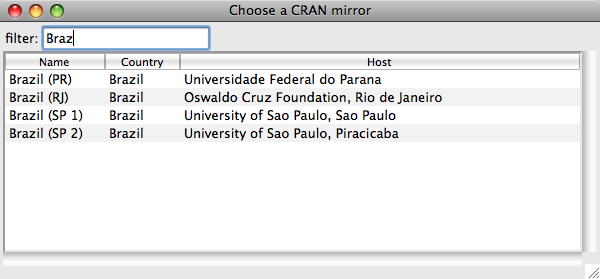
\includegraphics[width=.8\textwidth]{fig-tcltk-filter-table.png}
  \caption{Using \code{ttktreeview} to show various CRAN sites. This
    illustration adds a search-like box to filter what repositories
    are displayed for selection.}
  \label{fig:fig-tcltk-filter-table}
\end{figure}


The treeview  will only show the first three columns of the data frame, although we store the fourth which contains the URL.
\begin{Schunk}
\begin{Sinput}
 f1 <- ttkframe(f); tkpack(f1, expand=TRUE, fill="both")
 tr <- ttktreeview(f1, columns=1:ncol(df), 
                   displaycolumns = 1:(ncol(df) - 1), 
                   show = "headings",     # not "tree" 
                   selectmode = "browse") # single selection
 addScrollbars(f1, tr)
\end{Sinput}
\end{Schunk}

We configure the column widths and titles as follows:
\begin{Schunk}
\begin{Sinput}
 widths <- c(100, 75, 400)            # hard coded
 nms <- names(df)
 for(i in 1:3) {
   tcl(tr, "heading", i, text=nms[i])
   tcl(tr, "column", i, width=widths[i], 
       stretch=TRUE, anchor="w")
 }
\end{Sinput}
\end{Schunk}
%
The treeview widget does not do filtering internally.\footnote{The
  model-view-controller architecture of \GTK{} and \Qt, makes this task
  much easier, as it allows for an intermediate proxy model.} As such
we will replace all the values when filtering.  This following helper
function is used to fill in the widget with values from a data frame.
\begin{Schunk}
\begin{Sinput}
 fillTable <- function(tr, df) {
   children <- as.character(tcl(tr, "children", ""))
   for(i in children) tcl(tr, "delete", i)    # out with old
   shade <- c("none", "gray")
   for(i in seq_len(nrow(df))) 
     tcl(tr, "insert", "", "end", tag=shade[i %% 2], 
         text="",  
         values=unlist(df[i,]))               # in with new
   tktag.configure(tr, "gray", background="gray95")
 }
\end{Sinput}
\end{Schunk}
%
The initial call populates the table from the entire data frame.
\begin{Schunk}
\begin{Sinput}
 fillTable(tr, df)
\end{Sinput}
\end{Schunk}

The filter works by grepping the user input against the host value. We
bind to \Event{KeyRelease} (and not \Event{KeyPress}) so we capture the last keystroke.
\begin{Schunk}
\begin{Sinput}
 curInd <- 1:nrow(df)
 tkbind(filterEntry, "<KeyRelease>", function(W, K) {
   val <- tclvalue(tkget(W))
   possVals <- apply(df, 1, function(...) 
                     paste(..., collapse=" "))
   ind<- grep(val, possVals)
   if(length(ind) == 0) ind <- 1:nrow(df)
   fillTable(tr, df[ind,])
 })
\end{Sinput}
\end{Schunk}
%
This binding is for capturing a users selection through a double-click
event. In the callback, we set the CRAN option then withdraw the window.
\begin{Schunk}
\begin{Sinput}
 tkbind(tr, "<Double-Button-1>", function(W, x, y) {
   sel <- as.character(tcl(W, "identify", "row", x, y))
   vals <- tcl(W, "item", sel, "-values")
   URL <- as.character(vals)[4]          # not tclvalue
   repos <- getOption("repos")
   repos["CRAN"] <- gsub("/$", "", URL[1L])
   options(repos = repos)
   tkwm.withdraw(tkwinfo("toplevel", W))
 })
\end{Sinput}
\end{Schunk}
\end{example}

\begin{example}{A dialog for subsetting a data frame}{ex-tcltk-subset-dialog}
%% Make a subset filter for tcltk
%% Liviu Androvic
%
%
This longish example creates a framework for showing a list of similar
items, whose length is uncertain. There are several uses of such a framework. For example, a GUI
for formulas might have items given by terms between \code{+} values,
or a GUI for \pkg{ggplot2} might have items which represent individual
layers of a plot. Here we use the framework to create a dialog for the
\argument{subset}{subset} argument of the \function{subset}
function.\footnote{The author's would like to thank Liviu Andronic for
  ideas related to this example.} That argument
combines an arbitrary number of statements that produce logical values
to produce a logical index for a data frame. For our framework, each
item will produce one of these logical statements, and our list will
hold the items.
%
\begin{figure}
  \centering
  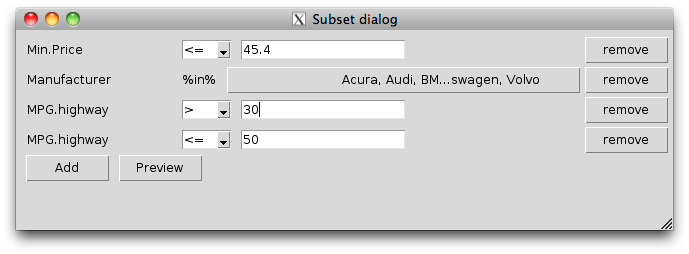
\includegraphics[width=.8\textwidth]{fig-tcltk-subset-filter.png}
  \caption{A dialog for subsetting a data frame}
  \label{fig:tcltk-subset-filter}
\end{figure}
%

To implement this, we first create a \class{FilterList} class. Our
class has a few properties: \code{df} to hold the data frame; \code{l}
to hold the list items; \code{id} to hold an internal counter to
reference the list items by; and \code{frame} to hold a
\code{ttkframe} instance, the parent container for each item.

%% Filter list reason
%% properties
\begin{Schunk}
\begin{Sinput}
 setOldClass("tkwin")
 setOldClass("tclVar")
 FilterList <- setRefClass("FilterList",
                           fields=list(
                             df="data.frame",
                             l="list",
                             id="integer",
                             frame="tkwin" 
                             ))
\end{Sinput}
\end{Schunk}
%% could pass back enc_frame so that we can pack or grid, but we avoid this.
%% add frame buffer so that we can ensure tkpack is okay The frame is where new items
%% will be placed.

The main interface for a filter list is limited. For management, we
define a method to \meth{add} a list item and one to \meth{remove} a
list item. We also need a method (\meth{get\_value}) to analyze the
items and produce a logical vector for subsetting the data frame with.
Beyond that we have methods to setup the GUI, a \meth{preview} method
to see the current subsetting, and a method to select a variable from
the data frame.


First, we define a method to setup our GUI. The \meth{initialize}
method will be passed a parent container. Here we pack in a frame
(\code{enc\_frame}) to hold the pieces of our GUI.\footnote{This
  means that \function{tkpack} needs to be used to manage any other
  children of this parent.  An alternative would be to pass back the
  enclosing frame object so that it can be managed as the user wants.}
These consist of a frame to hold the items and a frame to hold the
buttons. We use the \function{tkgrid} layout manager which allows us
to grow the top frame as needed, yet have the buttons receive the
additional expanding space.

\begin{Schunk}
\begin{Sinput}
 FilterList$methods(
           setup_gui = function(parent) {
             enc_frame <- ttkframe(parent, padding=5)
             tkpack(enc_frame, expand=TRUE, fill="both")
             frame <<- ttkframe(enc_frame)
             button_frame <- ttkframe(enc_frame)
             ## use grid to manage these
             tkgrid(frame, sticky="news")
             tkgrid(button_frame, sticky="new")
             tkgrid.rowconfigure(enc_frame, 1, weight=1)
             tkgrid.columnconfigure(enc_frame, 0, weight=1)
             ##
             addBtn <- 
               ttkbutton(button_frame, text="Add", 
                         command=function() .self$add())
             previewBtn <- 
               ttkbutton(button_frame, text="Preview", 
                         command=function() .self$preview())
             ##
             sapply(list(addBtn, previewBtn), tkpack, 
                    side="left", padx=5)
           })
\end{Sinput}
\end{Schunk}

The \meth{initialize} method simply initializes our fields and then
sets up the GUI. As the point of this is to filter a data frame, the
\code{df} argument has no default value and must be specified.

%% initialize sets the fields, setsup the GUI then returns
\begin{Schunk}
\begin{Sinput}
 FilterList$methods(
            initialize=function(df, parent, ...) {
              initFields(df=df, l=list(), id=0)
              setup_gui(parent)
              callSuper(...)
            })
\end{Sinput}
\end{Schunk}

Before showing a filter, we force the user to select a variable to
filter by. This selection involves choosing one from possibly many. A
table is an excellent choice for this, as it gracefully handles many
values. This convenience method provides a table selection widget in a
modal dialog window. Selection happens when a user selects one of the
rows of the table.

%% This helper function uses a table to select a single value from possible many
\begin{Schunk}
\begin{Sinput}
 FilterList$methods(
            select_variable=function() {
              "Return a variable name from the data frame"
              x <- sapply(df, function(i) class(i)[1])
              m <- cbind(Variables=names(x), Type=x)
              w <- tktoplevel()
              f <- ttkframe(w, padding=c(3,3,3,12))
              tkpack(f, expand=TRUE, fill="both")
              ##
              a <- populate_rectangular_treeview(f, m)
              tkconfigure(a$frame, width=300, height=200)
              tkpack(a$frame, expand=TRUE, fill="both")
              ## select a value, store in out
              out <- NA
              tkbind(a$tr, "<<TreeviewSelect>>", function(W) {
                sel <- tcl(W, "selection")
                val <- tcl(W, "item", sel, "-values")
                assign("out", as.character(val)[1], inherits=TRUE)
                tkdestroy(w)
              })
              tkwait.window(w)
              return(out)
            })
\end{Sinput}
\end{Schunk}
%% our main method to add a new variable. We can pass in a name, but
%% not from our GUI, where we use the just-defined select variable method
%% our new items will come from the newFilterItem yet to be defined. We see we pass in the values (for S3 dispatch), their name, a unique id and a reference to the filter list.

%% Comment, GUI might look nicer if we had use tkgrid here, but the add/remove is much easier using tkpack.

Our main add method has a few tasks: to select a variable, to create a
new filter item, to create a container, to do the internal
bookkeeping, and finally to call the items \code{make\_gui}
method. The \function{newFilterItem} call is an S3 generic used as a
factory method to find the correct filter item reference class to
produce an appropriate filter for the variable.
\begin{Schunk}
\begin{Sinput}
 FilterList$methods(
            add=function(varname, ...) {
              if(missing(varname)) 
                varname <- select_variable()
              x <- get(varname, df)
              ## new item
              id <<- id + 1
              item <- newFilterItem(x, varname, id, .self)
              ## make frame
              enc_frame <- ttkframe(frame)
              tkpack(enc_frame, expand=TRUE, fill="both", pady=2)
              l[[as.character(id)]] <<- list(frame=enc_frame, 
                                             item=item)
              item$make_gui(enc_frame)
            })
\end{Sinput}
\end{Schunk}
%

To remove an object requires us to remove it from our internal list
and from the GUI. We use \function{tkpack} to manage the items, so
\function{tkpack.forget} is used to remove the item. In the \code{add}
method we store the enclosing frame to make this task easy.
%% Remove an object means to remove from the GUI and to remove from the list. We use tkpack.forget for this.
\begin{Schunk}
\begin{Sinput}
 FilterList$methods(
            remove=function(id_obj, ...) {
              "Remove. id is character or item object"
              if(!is.character(id_obj))
                id_obj <- id_obj$id
              tkpack.forget(l[[id_obj]]$frame)
              l[[id_obj]] <<- NULL
            })
\end{Sinput}
\end{Schunk}
%

%% we need a method to query all the items, combine their values and
%% return that. Here is a simply way where we apply all to each
%% value. One could get fancier here by allowing the user to specify
%% and or or.

Here we query all the items and combine them to create a logical index
vector. The item interface described below will provide its own
\meth{get\_value} method so this task is a matter of combining the
results of each of those calls. We use \code{all} here, but if one
wanted to extend this GUI, one area would be to allow the user to
specify ``and'' or ``or'' between each item.
\begin{Schunk}
\begin{Sinput}
 FilterList$methods(
            get_value = function() {
              "Return logical value for all filter items"
              if(length(l) == 0)
                return(rep(TRUE, length=nrow(df)))
              ##
              out <- sapply(l, function(i) i$item$get_value())
              out[is.na(out)] <- FALSE   ## coerce NA to FALSE
              apply(out, 1, "all")
            })
\end{Sinput}
\end{Schunk}

The \meth{get\_value} method makes it easy to provide a \meth{preview}
method to show the current state of the subsetting. Basically we just
need to create a character matrix that we want to display and then use
our previously defined \function{populate\_rectangular\_treeview} function.

%% A simple preview to show the currently selected values. There is a bit of work here to convert
%% the values from a data.frame into a matrix.
\begin{Schunk}
\begin{Sinput}
 FilterList$methods(
            preview = function() {
              "Preview data frame"
              ind <- get_value()
              if(!any(ind)) {
                message("No matches")
                return()
              }
              ## coerce to character
              m <- df[ind,]
              for(i in seq_along(m)) m[,i] <- as.character(m[,i])
              ##
              w <- tktoplevel()
              f <- ttkframe(w, padding=c(3,3,3,12))
              tkpack(f, expand=TRUE, fill="both")
              a <- populate_rectangular_treeview(f, m)
              tkconfigure(a$frame, width=400, height=300)
              tkpack(a$frame, expand=TRUE, fill="both")
              ##
              btn <- ttkbutton(f, text="dismiss", 
                               command=function() tkdestroy(w))
              tkpack(btn, anchor="sw")
              tkwait.window(w)
            })
\end{Sinput}
\end{Schunk}

To use this new class, we would integrate it into a dialog, the basic
call needed would be something along the lines of the following:
\begin{Schunk}
\begin{Sinput}
 w <- tktoplevel()
 require(MASS)
 flist <- FilterList$new(df=Cars93, parent=w)
\end{Sinput}
\end{Schunk}
%
But before that will work, we need to define the filter item classes.


\paragraph{Filter items}
As mentioned, we use an S3 generic to select the reference class to provide the appropriate filter
item. These are still be be defined, but we show the default choice.

%% S3 method to pick correct filter
\begin{Schunk}
\begin{Sinput}
 newFilterItem <- function(x, nm=deparse(substitute(x)), id, 
                           list_ref) UseMethod("newFilterItem")
 newFilterItem.default <- function(x, nm=deparse(substitute(x)), 
                                   id, list_ref) 
   FilterItemNumeric$new(x=x, nm=nm, id=id, list_ref=list_ref)
\end{Sinput}
\end{Schunk}

A filter item needs to produce a logical vector used for indexing. At
a minimum we require a few properties: \code{x} to store the
variable's data that we are considering; \code{nm} to store the name
of this variable; \code{id} to store the id of where this item is
stored in the filter list; and \code{list\_ref} to store a reference
to the filter list. 


%% Basic interface for a filter item. the initialize method sets
%% values from the properties. The get_value method is called by the
%% Filter list's get_value method and must be defined. Remove simply
%% calls back into the list's remove item. The make_gui method here
%% just adds a remove button, the subclass can use this through a
%% callSuper call.
\begin{Schunk}
\begin{Sinput}
 FilterItem <- setRefClass("FilterItem",
                           fields=list(
                             x="ANY",
                             nm = "character",
                             id = "character",
                             list_ref="ANY"
                             ))
\end{Sinput}
\end{Schunk}

The filter item interface is not complicated. The most important method
is \code{get\_value} to return a logical variable. This was called by
the filter list's similarly named \code{get\_value} method. As well,
we call the item's \meth{make\_gui} method in the filter list. The
last method is simply a \code{remove} method which calls back up into the
\meth{remove} method of the item's parent filter list.

%% THe main interface for a filter item is defined below. The
%% FilterList calls its get_value method, the remove method simply
%% calls back into the parent, and the make_gui method sets up the
%% grapchial interface. This parent method simply adds the remove
%% button.
\begin{Schunk}
\begin{Sinput}
 FilterItem$methods(
            initialize=function(...) {
              initFields(...)
              .self
            },
            get_value = function() {
              "Return logical value of length x"
              stop("Must be subclassed")
            },
            remove=function() list_ref$remove(.self),
            make_gui = function(parent, ...) {
              "Set up GUI, including defining widgets"
              removeBtn <- ttkbutton(parent, text="remove",
                                     command=function() {
                                       .self$remove()
                                     })
              tkpack(removeBtn, side="right")
            })
\end{Sinput}
\end{Schunk}

The interesting things happen in the subclasses. For numeric values we
add two new properties to help with our \meth{get\_value} method: one
to store an inequality operator and one to store an expression the
user can enter.
%% classes
%% this has wo properties an inequality and a value to compare with. 
\begin{Schunk}
\begin{Sinput}
 FilterItemNumeric <- setRefClass("FilterItemNumeric",
                                  contains="FilterItem",
                                  fields=list(
                                    ineqVar="tclVar",
                                    valVar="tclVar"
                                    ))
\end{Sinput}
\end{Schunk}
%

With these two properties, our \meth{get\_value} method becomes a
matter of pasting together an expression then \iprogram{evaluating strings}evaluating it. We
evaluate this within the data frame so that \code{valVar} could use
variable names from the data framed. 
\begin{Schunk}
\begin{Sinput}
 FilterItemNumeric$methods(
       get_value = function() {
         xpr <- paste(nm, tclvalue(ineqVar), tclvalue(valVar))
         eval(parse(text=xpr), 
              envir=list_ref$df, parent.frame())
       })
 
\end{Sinput}
\end{Schunk}
%

Our GUI has three widgets a label, a combo box for the inequality
and an entry widget to put in values. One could simplify this, say
with a slider to slide through the possible values, but using an
entry widget gives more flexibility in the specification. We see that
we simply pack these widgets into the parent that is passed in to the method call.
\begin{Schunk}
\begin{Sinput}
 FilterItemNumeric$methods(
           make_gui = function(parent) {
             ## standard width for label
             labWidth <- max(sapply(names(list_ref$df), nchar))
             lab <- ttklabel(parent, text=nm, width=labWidth)
             ## ineq combo
             vals <- c(">=", ">", "==", "!=", "<", "<=")
             ineqVar <<- tclVar("<=")
             ineq <- ttkcombobox(parent, values=vals, 
                                 textvariable=ineqVar, width=4)
             ## entry
             valVar <<- tclVar(max(x, na.rm=TRUE))
             val <- ttkentry(parent, textvariable=valVar)
             ##
             sapply(list(lab, ineq, val), tkpack, side="left",
                    padx=5)
             callSuper(parent)
           })
 
\end{Sinput}
\end{Schunk}
%


The character selection class, also used with factors, is more
involved. Our \code{get\_value} method is basically \code{x \%in\%
  cur\_vals}, where \code{cur\_vals} is a selection from all possible
values.  We might want to use a group of checkboxes here, but that can
get unwieldy when there are more than a handful of
choices.\footnote{A table of checkboxes might also be used, but this
  isn't directly supported by the treeview widget of
  \pkg{tcltk}. Although, for the intrepid, one could set the image
  attribute for each row to show a check or non-check depending on the
  state.} We opt instead for a table selection widget. That can take
up vertical screen space. To avoid this we use a button which shows
the currently selected values, that can be clicked to open a dialog to
adjust these values. To keep a consistent horizontal size to these
buttons we ``ellipsize'' the button's text in the \code{ellipsize}
method. Some graphical toolkits, but not \Tk, have built-in
``ellipsize'' methods which prove useful when controlling space
allocations when translations are involved, as these can vary widely
in the number of characters needed to display.

For our new subclass, we have four additional properties, the tree
view for selection, the button, and vectors to store the possible
values and the currently selected values.
\begin{Schunk}
\begin{Sinput}
 FilterItemCharacter <- 
   setRefClass("FilterItemCharacter",
               contains="FilterItem",
               fields=list(
                 tr="tkwin",
                 btn="tkwin",
                 poss_vals="character",
                 cur_vals="character"
                 ))
\end{Sinput}
\end{Schunk}

As mentioned, our \meth{get\_value} method is easy to define:
\begin{Schunk}
\begin{Sinput}
 FilterItemCharacter$methods(
           get_value = function() {
             x %in% cur_vals
           })
\end{Sinput}
\end{Schunk}

The main work is in our \meth{select\_values\_dialog}, defined
below. We use the following helper function to preselect the currently
selected values when the dialog is opened.
\begin{Schunk}
\begin{Sinput}
 sel_by_name <- function(tr, nms) {
   all_ind <- as.character(tcl(tr, "children", ""))
   vals <- sapply(all_ind, function(i) {
     as.character(tcl(tr, "item", i, "-values"))
   })
   ind <- names(vals[vals %in% nms])
   sapply(ind, function(i) tcl(tr, "selection", "add", i))
   sapply(setdiff(all_ind, ind), 
          function(i) tcl(tr, "selection", "remove", i))
 }
\end{Sinput}
\end{Schunk}
%%

Here is our previously mentioned convenience method to make the button
size uniform by ``ellipsizing'' the button's label.
\begin{Schunk}
\begin{Sinput}
 FilterItemCharacter$methods(ellipsize = function() {
             tmp <- paste(cur_vals, collapse=", ")
             if((N <- nchar(tmp)) > 50)
               tmp <- sprintf("%s...%s", substr(tmp, 0, 15),
                              substr(tmp, N-12,N))
             sprintf("%50s", tmp)
           })
\end{Sinput}
\end{Schunk}
%

This is the main dialog to select values. Here multiple selection is
achieved by extending the selection through holding the \kbd{shift}
and \kbd{control} keys while clicking on items.

\begin{Schunk}
\begin{Sinput}
 FilterItemCharacter$methods(
           select_values_dialog=function() {
             w <- tktoplevel()
             f <- ttkframe(w, padding=c(3,3,12,12))
             tkpack(f, expand=TRUE, fill="both")
             tkpack(ttklabel(f, 
               text="Select values by extending selection"))
             ## selection
             m <- matrix(poss_vals); colnames(m) = "Values"
             a <- populate_rectangular_treeview(f, m)
             tkconfigure(a$tr, selectmode="extended")
             tkconfigure(a$frame, width=200, height=300)
             tkpack(a$frame, expand=TRUE, fill="both")
             
             sel_by_name(a$tr, cur_vals)         # see above
             
             tkbind(a$tr, "<<TreeviewSelect>>", function() {
               ind <- as.character(tcl(a$tr, "selection"))
               cur <- sapply(ind, function(i) {
                 as.character(tcl(a$tr, "item", i, "-values"))
               })
               if(length(cur) == 0)
                 cur <- character(0)
               cur_vals <<- cur
             })
             ## buttons
             f1 <- ttkframe(f); tkpack(f1)
             toggleBtn <- ttkbutton(f1, text="toggle", 
                          command=function() toggle_sel(a$tr))
             setBtn <- ttkbutton(f1, text="set", 
                          command=function() tkdestroy(w))
             sapply(list(toggleBtn, setBtn), tkpack, 
                    side="left", padx=5)
             ## make modal
             tkwait.window(w)
             tkconfigure(btn, text=ellipsize())
           })
\end{Sinput}
\end{Schunk}


Our main GUI for a character or factor item then has three widgets:
labels for the name and \code{\%in\%} operator and a button.
\begin{Schunk}
\begin{Sinput}
 FilterItemCharacter$methods(make_gui = function(parent) {
             poss_vals <<- sort(unique(as.character(x)))
             cur_vals <<- poss_vals
             ## label, ineq, val
             labWidth <- max(sapply(names(list_ref$df), nchar))
             lab <- ttklabel(parent, text=nm, width=labWidth)
             ##
             inLab <- ttklabel(parent, text="%in%")
             ##
             btn <<- ttkbutton(parent, text=ellipsize(), 
                        command=.self$select_values_dialog)
             ##
             sapply(list(lab, inLab), tkpack,
                    side="left", padx=5)
             tkpack(btn, expand=TRUE, fill="x", side="left")
             callSuper(parent)
           })
\end{Sinput}
\end{Schunk}


We leave it as an exercise for the reader to add a subclass for
logical variables or date variables.

\end{example}



%% Comment on tktable XXX Do I want more XXX

\subsection{Editable tables of data}
\label{sec:editable-tables-data}

There is no native widget for editing the cells of tabular data, as is
provided by the \function{edit} method for data frames. The
\code{tktable} widget (\url{http://tktable.sourceforge.net/}) provides
such an add-on to the base \TK. We don't illustrate its usage here, as
we keep to the core set of functions provided by \TK.  An interface
for this \TCL\/ package is provided in the \pkg{tcltk2} package
(\function{tk2edit}).  The \code{gdf} function of \pkg{gWidgetstcltk}
is based on this.



\subsection{Hierarchical data}

Specifying tree-like or hierarchical data is nearly identical to
specifying rectangular data for the \code{ttktreeview} widget.  The
widget provides column \code{\#0} to display this extra structure. If
an item, except the root, has children, a trigger icon to expand the
tree is shown. This is in addition to any text and/or an icon that is
specified. Children are displayed in an indented manner to indicate
the level of ancestry they have relative to the root.  To insert
hierarchical data into the widget the same
\subcommand{insert}{ttktreeview} subcommand is used, only instead of
using the root item, \qcode{}, as the parent item, one uses the item
ID corresponding to the desired parent. If the option \code{open=TRUE}
is specified to the \code{insert} subcommand, the children of the item
will appear, if \code{FALSE}, the user can click the trigger icon to
see the children. The programmer can use the
\subcommand{item}{ttktreeview} to configure this state. When the
parent item is opened or closed, the virtual events
\VirtualEvent{TreeviewOpen} and \VirtualEvent{TreeviewClose} will be
signaled.

%% example?
%% tcl(tr, "insert","I001","end", text="child", open=FALSE)
%% tcl(tr, item, "I001", open=TRUE)

%% traversal 

\paragraph{Traversal}
Once a tree is constructed, the programmer can traverse
through the items using the subcommands
\subcommanda{parent}{ttktreeview}{item} to get the ID for the parent of the
item; \subcommanda{prev}{ttktreeview}{item} and
\subcommanda{next}{ttktreeview}{item} to get the immediate siblings of the
item; and \subcommanda{children}{ttktreeview}{item} to return the children of
the item. Again, the latter one will produce a character vector of  IDs for the
children when coerced to character with \code{as.character}.



%% tree example using XML
\begin{example}{Using the treeview widget to show an XML file}{ex-tcltk-tree}
This example shows how to display the hierarchical structure of an XML
document using the tree widget.

We use the \pkg{XML} library to parse a document from the
internet. This example uses just a few functions from this library:
The \function(htmlTreeParse) (similar to \function{xmlInternalTreeParse}) to parse the file, 
\function{xmlRoot} to find the base node,
\function{xmlName} to get the name of a node, 
\function{xmlValue} to get an associated value, and
\function{xmlChildren} to return any child nodes of a node.



\begin{figure}
  \centering
  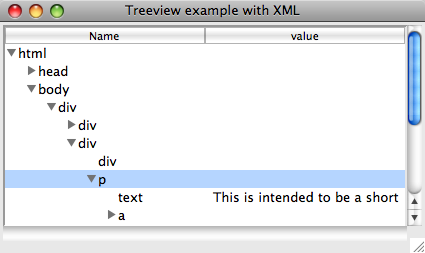
\includegraphics[width=.7\textwidth]{fig-tcltk-xml-viewer.png}
  \caption{Illustration of using \code{ttktreeview} widget to show
    hierarchical data returned from parsing an HTML document with the
    \pkg{XML} package.}
  \label{fig:fig-tcltk-xml-viewer}
\end{figure}
\begin{Schunk}
\begin{Sinput}
 library(XML)
 fileName <- "http://www.omegahat.org/RSXML/shortIntro.html"
 QT <- function(...) {}  # quiet next call
 doc <- htmlTreeParse(fileName, useInternalNodes=TRUE, error=QT)
 root <- xmlRoot(doc)
\end{Sinput}
\end{Schunk}
Our GUI is primitive, with just a treeview instance added.
\begin{Schunk}
\begin{Sinput}
 tr <- ttktreeview(f, displaycolumns="#all", columns=1)
 addScrollbars(f, tr)                    
\end{Sinput}
\end{Schunk}

We configure our column headers and set a minimum
width below. Recall, the tree column is designated \qcode{\#0}.
\begin{Schunk}
\begin{Sinput}
 tcl(tr, "heading", "#0", text="Name")
 tcl(tr, "column", "#0", minwidth=20)
 tcl(tr, "heading", 1, text="value")
 tcl(tr, "column", 1, minwidth=20)
\end{Sinput}
\end{Schunk}

To map the tree-like structure of the XML document into the widget, we
define the following function to recursively add to the treeview
instance.  We only add to the \code{value} column (through the
\code{values} option) when the node does not have children. We use
\code{do.call}, as a convenience, to avoid constructing two different
calls to the \code{insert} subcommand. 
\begin{Schunk}
\begin{Sinput}
 insertChild <- function(tr, node, parent="") {
   l <- list(tr, "insert", parent, "end", text=xmlName(node))
   children <- xmlChildren(node)
   if(length(children) == 0) {         # add in values
     values <- paste(xmlValue(node), sep=" ", collapse=" ")
     l$values <- as.tclObj(values)     # avoid split on spaces
   }
   treePath <- do.call("tcl", l)
 
   if(length(children))                          # recurse
     for(i in children) insertChild(tr, i, treePath)
 }
 insertChild(tr, root)
\end{Sinput}
\end{Schunk}
%
At this point, the GUI will allow one to explore the markup structure of the
XML file. We continue this example to show two things of general
interest, but that are really artificial for this example.

%%\XXX{Use index parent to place at same level just below}

\paragraph{Drag and drop}
First, we show how one might introduce drag and drop to rearrange the
rows. We begin by defining two global variables that store the row
that is being dragged  and a flag to indicate if a drag event is ongoing.
\begin{Schunk}
\begin{Sinput}
 .selectedID <- ""                               # globals
 .dragging <- FALSE
\end{Sinput}
\end{Schunk}
We provide callbacks for three events: a mouse click, mouse motion and mouse release.
This first callback sets the selected row on a mouse click.
\begin{Schunk}
\begin{Sinput}
 tkbind(tr, "<Button-1>", function(W,x,y) {
   .selectedID <<- as.character(tcl(W, "identify","row", x, y))
 })  
\end{Sinput}
\end{Schunk}
The motion callback configures the cursor to indicate a drag event and sets
the dragging flag. One might also put in code to highlight
any drop areas.
\begin{Schunk}
\begin{Sinput}
 tkbind(tr, "<B1-Motion>", function(W, x, y, X, Y) {
   tkconfigure(W, cursor="diamond_cross")
   .dragging <<-TRUE
 })
\end{Sinput}
\end{Schunk}

When the mouse button is released we check that the widget we are over
is indeed the tree widget. If so, we then move the rows. One can't
move a parent to be a child of its own children, so we wrap the
\subcommand{move}{ttktreeview} sub command within \code{try}. The
\code{move} command places the new value as the first child of the
item it is being dropped on. If a different action is desired, the
\qcode{0} below would need to be modified.
\begin{Schunk}
\begin{Sinput}
 tkbind(tr, "<ButtonRelease-1>", function(W, x, y, X, Y) {
   if(.dragging && .selectedID != "") {
     w = tkwinfo("containing", X, Y)
     if(as.character(w) == as.character(W)) {
       dropID <- as.character(tcl(W, "identify","row", x, y))
       try(tkmove(W, .selectedID, dropID, "0"), silent=TRUE)
     }
   }
   .dragging <<- FALSE; .selectedID <<- "" # reset
 })
\end{Sinput}
\end{Schunk}

\paragraph{Walking the tree}
Our last item of general interest is a function that shows one way to
walk the structure of the treeview widget to generate a list
representing the structure of the data.  A potential use of this might
be to allow a user to rearrange an XML document through drag and drop.
The subcommand \subcommand{children}{ttktreeview} proves useful here,
as it is used to identify the hierarchical structure. When there are children a recursive call is made.



\begin{Schunk}
\begin{Sinput}
 treeToList <- function(tr) {
   l <- list()
   walkTree <- function(child, l) {
     l$name <- tclvalue(tcl(tr,"item", child, "-text"))
     l$value <- as.character(tcl(tr,"item", child, "-values"))
     children <- as.character(tcl(tr, "children", child)) 
     if(length(children)) {
       l$children <- list()
       for(i in children) 
         l$children[[i]] <- walkTree(i, list()) # recurse
     }
     return(l)
   }
   walkTree("", l)
 }
 
\end{Sinput}
\end{Schunk}
\end{example}

\section{Canvas widget}
\label{sec:tcltk:canvas-widget}

 
The canvas widget provides an area to display lines, shapes, images
and widgets. The canvas widget is quite complicated and we content
ourselves to describing a subset of its possiblities. For an excellent
example of how it can be used to provide a useful GUI for \R{} see the
\pkg{RnavGraph} package by Waddell and Oldford.


As described on its manual page, the canvas widget implements
structured graphics, displaying any number of items or objects of
various types.  Methods exist to create, move and delete these
objects, allowing the canvas widget to be the basis for creating
interactive GUIs. The constructor \constructor{tkcanvas} for the
widget, being a non-themeable widget, has many arguments including
these standard ones: \argument{width}{tkcanvas},
\argument{height}{tkcanvas}, \argument{background}{tkcanvas},
\argument{xscrollcommand}{tkcanvas} and
\argument{yscrollcommand}{tkcanvas}.


\paragraph{The create command}
The subcommand \subcommanda{create}{tkcanvas}{type [options]} is used
to add new items to the canvas. The options vary with the type of the
item. The basic shape types that one can add are \qcode{line},
\qcode{arc}, \qcode{polygon}, \qcode{rectangle}, and
\qcode{oval}. Their options specify the size using $x$ and $y$
coordinates. Other options allow one to specify colors, etc. The
complete list is covered in the \code{canvas} manual page, which we
refer the reader to, as the description is lengthy.  In the examples,
we show how to use the \qcode{line} type to display a graph and how to
use the \qcode{oval} type to add a point to a canvas. Additionally,
one can add text items through the \qcode{text} type. The first
options are the $x$ and $y$ coordinates and the \code{text} option
specifies the text.  Other standard text options are possible (e.g.,
\code{font}, \code{justify}, \code{anchor}).

The type can also be an image object or a widget (a window
object). Images are added by specifying an $x$ and $y$ position,
possibly an anchor position, and a value for the \qcode{image} option
and optionally, for state dependent display, specifying
\qcode{activeimage} and \qcode{disabledimage} values. The
\qcode{state} option is used to specify the current state. Window
objects are added similarly in terms of their positioning, along with
options for \qcode{width} and \qcode{height}. The window itself is
added through the \qcode{window} option. An example shows how to add a
frame widget.

% Once created, a screenshot of the canvas can be created through the
% \subcommand{postscript}{tkcanvas} subcommand, as in
% \code{tcl(canvas, "postscript", file="filename")}. To store the
% widget so that it can be recreated is not supported directly. \TCL\/
% code to do so can be found at \url{http://wiki.tcl.tk/9168}.


\paragraph{Items and tags}
The \code{tkcanvas.create} function returns an item ID. This can be
used to refer to the item at a later stage. Optionally, tags can be
used to group items into common groups. The \qcode{tags} option can be
used with \code{tkcreate} when the item is created, or the
\subcommand{addtag}{tkcanvas} subcommand can be used. The call
\code{tkaddtag(canvas, tagName, "withtag", item)} would add the tag
``\code{tagName}''to the \code{item} returned by \code{tkcreate}. (The
\qcode{withtag} is one of several search specifications.) As well, if
one is adding a tag through a mouse click, the call \code{tkaddtag(W,
  "tagName", "closest", x, y)} could be used with \code{W}, \code{x}
and \code{y} coming from percent substitutions. Tags can be deleted
through the \subcommanda{dtag}{tkcanvas}{tag} subcommand.

%% interaction with items
There are several subcommands that can be called on items as specified
by a tag or item ID. For example, the \subcommand{itemcget}{tkcanvas}
and \subcommand{itemconfigure}{tkcanvas} subcommands allow one to get
and set options for a given item. The
\subcommanda{delete}{tkcanvas}{tag\_or\_ID} subcommand can be used to
delete an item. Items can be moved and scaled but not rotated. The
\subcommanda{move}{tkcanvas}{tag\_or\_ID x y} subcommand implements
incremental moves (where $x$ and $y$ specify the horizontal and
vertical shift in pixels). The subcommand
\subcommanda{coords}{tkcanvas}{ tag\_or\_ID [coordinates]} allows one
to respecify the coordinates for the item. The
\subcommand{scale}{tkcanvas} command is used to rescale items. Except
for window objects, an item can be raised to be on top of the others
through the \subcommanda{raise}{tkcanvas}{item\_or\_ID} subcommand.



\paragraph{Bindings}
As usual, bindings can be specified overall for the canvas, through
\code{tkbind}. However, bindings can also be set on specific items
through the subcommand \subcommanda{bind}{tkcanvas}{tag\_or\_ID event
  function} (or with \code{tkitembind}). This allows bindings to be
placed on items sharing a tag name, without having the binding on all
items. Only mouse, keyboard or virtual events can have such bindings.

%% do with fonts now
\begin{example}{Using a canvas to make a scrollable frame}{ex:tcltk-scrollable-frame}
%%
This example\footnote{This example is modified from an example found
  at \url{
    http://mail.python.org/pipermail/python-list/1999-June/005180.html}}
shows how to use a canvas widget to create a box container that
scrolls when more items are added than will fit in the display
area. The basic idea is that a frame is added to the canvas equipped
with scrollbars using the \subcommand{create window}{tkcanvas}
subcommand. 

There are two bindings to the \Event{Configure} event. The first
updates the scroll region of the canvas widget to include the entire
canvas, which grows as items are added to the frame. The second
binding ensures the child window is the appropriate width when the
canvas widget resizes. The height is not adjusted, as this is
controlled by the scrolling.

\begin{Schunk}
\begin{Sinput}
 scrollableFrame <- function(parent, width= 300, height=300) {
   canvasWidget <- 
     tkcanvas(parent,
              borderwidth=0, highlightthickness=0,
              width=width, height=height)
   addScrollbars(parent, canvasWidget)
   #
   gp <- ttkframe(canvasWidget, padding=c(0,0,0,0))
   gpID <- tkcreate(canvasWidget, "window", 0, 0, anchor="nw", 
                    window=gp)
   tkitemconfigure(canvasWidget, gpID, width=width)
   ## update scroll region
   tkbind(gp,"<Configure>",function() {  
     bbox <- tcl(canvasWidget, "bbox", "all")
     tcl(canvasWidget,"config", scrollregion=bbox)
   })
   ## adjust "window" width when canvas is resized.
   tkbind(canvasWidget, "<Configure>", function(W) {
     width <- as.numeric(tkwinfo("width", W))
     gpwidth <- as.numeric(tkwinfo("width", gp))
     if(gpwidth < width)
       tkitemconfigure(canvasWidget, gpID, width=width)
   })
   return(gp)
 }
\end{Sinput}
\end{Schunk}

To use this, we create a simple GUI as follows:
\begin{Schunk}
\begin{Sinput}
 w <- tktoplevel()
 tkwm.title(w,"Scrollable frame example")
 g <- ttkframe(w); tkpack(g, expand=TRUE, fill="both")
 gp <- scrollableFrame(g, 300, 300)
\end{Sinput}
\end{Schunk}

To display a collection of available fonts requires a widget or
container that could possibly show hundreds of similar values. The
scrollable frame serves this purpose well
(cf. Figure~\ref{fig:fig-tcltk-all-fonts}).  The following shows how a
label can be added to the frame whose font is the same as the label
text. The available fonts are found from \function{tkfont.families}
and the useful coercion to character by \function{as.character}.
\begin{Schunk}
\begin{Sinput}
 fFamilies <- as.character(tkfont.families())
 ## skip odd named ones
 fFamilies <- fFamilies[grepl("^[[:alpha:]]", fFamilies)] 
 for(i in seq_along(fFamilies)) {
   fName <- sprintf("::font::-%s", i)
   try(tkfont.create(fName, family=fFamilies[i], size=14), 
       silent=TRUE)
   l <- ttklabel(gp, text=fFamilies[i], font=fName)
   tkpack(l, side="top", anchor="w")
 }
\end{Sinput}
\end{Schunk}

\end{example}

%% example with lines objects
\begin{example}{Using canvas objects to show sparklines}{ex-tcltk-sparklines}
Edward Tufte, in his book \textit{Beautiful
  Evidence}~\footcite{Tufte:Beautiful-Evidence}, advocates for the use of
\textit{sparklines} -- small, intense, simple datawords -- to show substantial
amounts of data in a small visual space. This example shows how to use
a \code{tkcanvas} object to display a sparkline graph using a \texttt{line} object. The example also uses \texttt{tkgrid}
to layout the information in a  table. We could have spent more time on the
formatting of the numeric values and factoring out the data download, but leave improvements as an exercise.


\begin{figure}
  \centering
  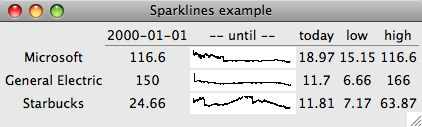
\includegraphics[width=0.66\textwidth]{fig-tcltk-sparklines.png}
  \caption{Example of embedding sparklines in a display organized
    using \code{tkgrid}. A \code{tkcanvas} widget is used to display
    the graph.}
  \label{fig:fig-tcltk-sparklines}
\end{figure}


This function simply shortens our call to \texttt{ttklabel}. We use
the global \texttt{f} (a \code{ttkframe}) as the parent.
\begin{Schunk}
\begin{Sinput}
 mL <- function(label) { # save some typing
   if(is.numeric(label))
     label <- sprintf("%.2f", label)
   ttklabel(f, text=label, justify="right") 
 }
\end{Sinput}
\end{Schunk}
%
We begin by making the table header along with a toprule.
\begin{Schunk}
\begin{Sinput}
 tkgrid(mL(""), mL("2000-01-01"), mL("-- until --"), 
        mL("today"), mL("low"), mL("high"))
 tkgrid(ttkseparator(f), row=1, column=1, columnspan=5, 
        sticky="we")
\end{Sinput}
\end{Schunk}
%
This function adds a sparkline to the table. A sparkline here is just
a line item, but there is some work to do, in order to scale the
values to fit the allocated space. This example uses stock values, as
we can conveniently employ the \function{get.hist.quote} function from
the \pkg{tseries} package to get interesting data.
\begin{Schunk}
\begin{Sinput}
 addSparkLine <- function(label, symbol="MSFT") {
   width <- 100; height=15               # fix width, height
   y <- get.hist.quote(instrument=symbol, start="2000-01-01",
                       quote="C", provider="yahoo", 
                       retclass="zoo")$Close
   min <- min(y); max <- max(y)
   ##
   start <- y[1]; end <- tail(y,n=1)
   rng <- range(y)
   ##
   sparkLineCanvas <- tkcanvas(f, width=width, height=height)
   x <- 0:(length(y)-1) * width/length(y)
   if(diff(rng) != 0) {
     y1 <- (y - rng[1])/diff(rng) * height
     y1 <- height - y1   # adjust to canvas coordinates
   } else {
     y1 <- height/2 + 0 * y
   }
   ## make line with: pathName create line x1 y1... xn yn 
   l <- list(sparkLineCanvas,"create","line")
   sapply(seq_along(x), function(i) {
     l[[2*i + 2]] <<- x[i]
     l[[2*i + 3]] <<- y1[i]
   })
   do.call("tcl",l)
 
   tkgrid(mL(label),mL(start), sparkLineCanvas, 
          mL(end), mL(min), mL(max), pady=2, sticky="e")
 }
\end{Sinput}
\end{Schunk}

We can then add some rows to the table as follows:
\begin{Schunk}
\begin{Sinput}
 addSparkLine("Microsoft","MSFT")
 addSparkLine("General Electric", "GE")
 addSparkLine("Starbucks","SBUX")
\end{Sinput}
\end{Schunk}
\end{example}

%% Moving an object
\begin{example}{Capturing mouse movements}{ex-tcltk-canvas}
This example is a stripped-down version of the \code{tkcanvas.R} demo
that accompanies the \pkg{tcltk} package. That example shows a
scatterplot with regression line. The user can move the points around
and see the effect this has on the scatterplot. Here we focus on the
moving of an object on a canvas widget. We assume we have such a
widget in the variable \code{canvas}.


This following adds a single point to the canvas using an
\code{oval} object. We add the \qcode{point} tag to this item, for
later use. Clearly, this code could be modified to add more points.
\begin{Schunk}
\begin{Sinput}
 x <- 200; y <- 150; r <- 6
 item <- tkcreate(canvas, "oval", x - r, y - r, x + r, y + r,
                  width=1, outline="black",
                  fill="blue")
 tkaddtag(canvas, "point", "withtag", item)
\end{Sinput}
\end{Schunk}

In order to indicate to the user that a point is active, in some
sense, the following changes the fill color of the point when the
mouse hovers over. We add this binding using \code{tkitembind}
so that is will apply to all point items and only the point items.
\begin{Schunk}
\begin{Sinput}
 tkitembind(canvas, "point", "<Any-Enter>", function()
            tkitemconfigure(canvas, "current", fill="red"))
 tkitembind(canvas, "point", "<Any-Leave>", function()
            tkitemconfigure(canvas, "current", fill="blue"))
\end{Sinput}
\end{Schunk}

There are two key bindings needed for movement of an object. First, we
tag the point item that gets selected when a mouse clicks on a point
and update the last position of the currently selected point.
\begin{Schunk}
\begin{Sinput}
 lastPos <- numeric(2)            # global to track position
 tagSelected <- function(W, x, y) {
   tkaddtag(W,  "selected",  "withtag",  "current")
   tkitemraise(W, "current")
   lastPos <<- as.numeric(c(x, y))
 }
 tkitembind(canvas, "point", "<Button-1>",  tagSelected)
\end{Sinput}
\end{Schunk}

When the mouse moves, we use \code{tkmove} to have the currently
selected point move too. As \code{tkmove} is parameterized by
differences, we track the differences
between the last position recorded and the current position.
\begin{Schunk}
\begin{Sinput}
 moveSelected <- function(W, x, y) {
   pos <- as.numeric(c(x,y))
   tkmove(W, "selected", pos[1] - lastPos[1], 
                         pos[2] - lastPos[2])
   lastPos <<- pos
 }
 tkbind(canvas, "<B1-Motion>", moveSelected)
\end{Sinput}
\end{Schunk}
%
A further binding, for the \Event{ButtonRelease-1} event, would be
added to do something after the point is released. In the original
example, the old regression line is deleted, and a new one drawn. Here
we simply delete the \qcode{selected} tag.
\begin{Schunk}
\begin{Sinput}
 tkbind(canvas, "<ButtonRelease-1>", 
        function(W) tkdtag(W,"selected"))
\end{Sinput}
\end{Schunk}


\end{example}



